%% The openany option is here just to remove the blank pages before a new chapter
\documentclass[11pt,openany]{book}

\title{Memoria DreamStill}

\usepackage{pagenote}
\usepackage[english,spanish]{babel}
\usepackage[utf8]{inputenc}
\usepackage{graphicx} 
\usepackage{hyperref,xcolor}
\usepackage{cite}
\usepackage{float}
\usepackage{pdfpages}
\usepackage{booktabs}
\usepackage{enumitem}
\usepackage{blindtext}
\usepackage{array}
\usepackage{array}
\usepackage{longtable}

%%%%%%%%%%%%% For customising the endnote markers. Comment these out if you don't want them.
% To prefix each note number with the chapter number
\renewcommand{\thepagenote}{\thechapter-\arabic{pagenote}}

% To have a slightly different formatting for the endnote numbers in the text -- smaller text, sans-serif, square brackets
\renewcommand\notenumintext[1]{\space{\footnotesize\sffamily[FN-#1]}}

% To have a slightly different formatting for the endnote numbers in the notes section. Just the square brackets and sans-serif; normal size.
\renewcommand\notenuminnotes[1]{{\sffamily[FN-#1] }}

% If you want a different name/heading for the end notes
\renewcommand{\notesname}{End Notes}
\addto\captionsspanish{\renewcommand{\bibname}{Referencias}}
\renewcommand{\figurename}{Fig.}
\renewcommand{\bibname}{Referencias}

% Custom commands

\newcommand{\logo}[2]{\medskip\begin{center}\includegraphics[totalheight=2cm]{#1}\\\scriptsize\url{#2}\end{center}\bigskip}
\renewcommand\UrlFont{\color{black}\rmfamily\itshape}
\setlength{\parindent}{4em}
\setlength{\parskip}{1em}
\newcolumntype{M}[1]{>{\centering\arraybackslash}m{#1}}

%%%%%%%%%%%%% End customisation


%% THIS LINE IS MANDATORY
\makepagenote

\begin{document}
 \begin{titlepage}
 \centering
  
\includegraphics[scale=2.5]{logos/us}	

 \begin{center}\bf\sffamily
 
  {\normalsize ESCUELA T{\'E}CNICA SUPERIOR DE INGENIER{\'I}A INFORM{\'A}TICA}\\[1.5cm]
  {\large Proyecto fin de Carrera Grado}\\[1cm]
  {\large Ingeniería Del Software}\\[2cm]
  {\large DreamStill}\\[1.5cm]
  {\large Realizado por}\\
  {\large Juan Ramón Rodríguez Rosado}\\
  [1cm]
  {\large Dirigido por}\\
  {\large D. José Antonio Parejo Maestre}\\[1cm]
  {\large Departamento}\\
  {\large Lenguajes y Sistemas Informáticos}   
\end{center}
\vfill
 \begin{flushright}
  {\bf\sffamily\large Sevilla, {\large 14 de Marzo de 2017}}
 \end{flushright}

\end{titlepage}

% \begin{titlepage}
% \begin{center}
% Proyecto Fin de Carrera \\
% Escuela Técnica Superior de Ingeniería Informática \\
% \vspace*{1 in}
% \huge{Memoria Trabajo de Fin de Grado \\ DreamStill }
% \end{center}
% \bigskip
% \begin{center}
% 
\includegraphics[totalheight=6cm]{logos/sello.png}
% \end{center}
% \begin{flushright}
% \begin{tabular}{ll}
% \textit{\textbf{Alumno}} &: Juan Ramón Rodríguez Rosado \\
% \textit{\textbf{Tutor}} &: D. José Antonio Parejo Maestre \\
% \textbf{\textit{Grupo}} &: N Grupo \\
% \textbf{\textit{Fecha}} &: dd/mm/aaaa \\
% \end{tabular}
% \end{flushright}
% \bigskip
% \vspace*{0.6 in}
% \begin{center}
% \sc Universidad de Sevilla\\
% \sc Ingeniería Informática Ingeniería del Software \\
% \sc TFG -- 4º IS
% \end{center}
% \end{titlepage}


\tableofcontents % indice de contenidos
\addcontentsline{toc}{chapter}{Lista de figuras} % para que aparezca en el indice de contenidos
\listoffigures % indice de figuras
\cleardoublepage
\addcontentsline{toc}{chapter}{Lista de tablas} % para que aparezca en el indice de contenidos
\listoftables % indice de tablas

%1.Introducción (Respondemos a:
% - ¿Cuál es el problema?
% - ¿Por qué es un problema interesante?
% - ¿Qué solución le hemos dado?
% - ¿Por qué es una solución interesante? ¿Qué se diferencia de las soluciones existentes?
% )
\chapter{Introducción}

El estilo de vida moderno conlleva un ritmo frenético de las tareas que realizamos, provocando un cambio en las costumbres actuales. Sin embargo, hay actividades que han de mantenerse, ya que el descuido de las mismas tiene consecuencias desfavorables para nuestra salud. Entre éstas actividades encontramos la alimentación, el deporte y el descanso entre muchas otras. Es en ésta última actividad en la que se va a centrar el presente proyecto.

¿Sería usted capaz de responderme cuántas horas duerme normalmente? ¿Cree que duerme las horas suficientes? Probablemente no sea capaz de responder a estas preguntas, porque actualmente, debido a nuestra vida ajetreada o a la inclusión de otras actividades, no le damos la suficiente importancia al descanso. Teóricamente se deben dormir de media, dependiendo de la edad por supuesto, entre siete y nueve horas \cite{1}. Sin embargo, ¿Cree que usted cumple con esa media?

Además, el tema de la monitorización del sueño o en inglés ``Sleep Tracking'' se encuentra en auge, ya que con las nuevas tecnologías podemos realizar un seguimiento más exacto y sencillo de nuestras actividades físicas, nuestra nutrición o nuestro descanso. Ésto despierta mucho interés entre los usuarios que desean llevar un estilo de vida saludable y que desean mejorar sus hábitos para mejorar su calidad de vida. 

Debido a éste problema, actualmente existen diversas soluciones que permiten medir nuestro sueño, tanto en términos de cantidad de horas como de calidad del mismo. Pero muchas de éstas soluciones son privativas y necesitan de una plataforma o aplicación específica. Así, un usuario que cambia por ejemplo de smartwatch, pulsómetro o incluso de Smartphone, una práctica bastante habitual hoy día \cite{17}, o al que le surge la necesidad de consultar sus datos desde su ordenador, puede no llegar a tener acceso a los datos de su propio sueño, ya que necesitará una aplicación que sólo se ejecuta en determinadas plataformas. 

\section{El problema}

El problema reside en un principio en la variedad de plataformas móviles, ya que dependiendo del Sistema Operativo que tengamos en nuestro Smartphone tendremos acceso a los datos de unas u otras aplicaciones. 

El proyecto nace con la idea de eliminar ésta barrera y dar soporte a todos los usuarios sin importar de que plataforma accedan mediante una aplicación web, por lo que cualquier usuario con un navegador web instalado pueda acceder a sus propios datos de sueño.

Además, nos encontramos con problemas a la hora de revisar nuestro datos de sueño, ya que en unas aplicaciones los datos son muy detallados pero carecen de funcionalidad, y en otras, ofrecen éstas funcionalidades pero el detalle que ofrecen en la aplicación no es suficiente, sin olvidar la falta de homogeneidad entre unas y otras. También, nos encontramos con las carencias a la hora de mostrar los datos obtenidos de las distintas fuentes, por ejemplo, aplicaciones como Google Fit o Apple Health se limitan a mostrar el intervalo de sueño de ese usuario, es decir, la hora a la que se quedó dormido/a y la hora a la que se despertó, sin ofrecer mayor información, aún cuando los datos detallados están disponibles.

Por tanto nuestra propuesta se basará en tres pilares fundamentales: resolver el problema de la diversidad de plataformas y abstraer al usuario que utilice la aplicación de dicha diversidad, agrupar en una sola aplicación todos los reportes que ofrecen algunas plataformas sin necesidad de que el usuario tenga que consultarlos diariamente y añadir mayor información a los reportes que utilizan distintas plataformas sobre el sueño de un usuario en la aplicación de la misma, en base a los datos reales de monitorización capturados.

\section{La solución}

El presente proyecto tiene la finalidad de mostrarle a los usuarios su calidad de sueño, cuantas horas han dormido, en qué estado y una representación de estos datos de tal forma que puedan intuirlos de ``un vistazo''. Además, la aplicación que se va a desarrollar será transparente a los cambios entre aplicaciones de medimiento de sueño, ya que podrá obtener todos los datos tanto de una aplicación u otra.

La solución consiste en crear una aplicación web, a la que el usuario podrá acceder y revisar sus distintos ``eventos''. Se conocerá como evento toda aquella actividad recopilada de otras aplicaciones en las que el usuario ha registrado una actividad de sueño. Ésta aplicación web dará a los usuarios de manera sencilla la posibilidad de integrarse con distintas aplicaciones. Con ésta solución se pretende que el usuario de una manera simple pueda ver los datos de ambas aplicaciones sin tener la necesidad de ira a buscarlo a fuentes distintas. Para que la interfaz resulte lo más intuitiva posible, se creará un calendario en la vista principal, desde el que el usuario que acceda a la aplicación podrá ver los eventos que han sido extraídos de las distintas fuentes representados en los días de éste calendario y podrá ir accediendo individualmente a cada uno de ellos sin la necesidad de verlos detalladamente todos. 

Dentro de cada evento anteriormente comentado, el usuario se encontrará con dos gráficas. La primera de ellas representará los movimientos o estados (siendo el estado: durmiendo, inquieto o despierto) que ha generado el usuario durante sus horas de sueño. La segunda gráfica, representará la calidad del sueño ofreciendo un resumen de cada uno de los estados por los que el usuario ha pasado a lo largo de la actividad y dando una idea de como ha sido la calidad de sueño general de ese usuario.

El interés de ésta solución se encuentra en ofrecerle a los usuarios potenciales de la aplicación, tener una aplicación multiplataforma que recoge datos de distintas fuentes, posibilitándole a aquellos usuarios que tienen varios dispositivos para el registro de sus actividades físicas o que quieren tener una sola aplicación para la visualización de los datos del mismo, el no necesitar cambiar entre aplicaciones para ver los datos de una u otra.

Respecto al resto de alternativas, nos diferenciamos en distintos aspectos. El primero es que algunas aplicaciones se restringen a los sistemas operativos para los que han sido desarrollados, nuestra aplicación, al tratarse de una aplicación web no tendría éste problema. Por otro lado, no todas las fuentes se sincronizan con las aplicaciones que traen los sistemas operativos para el registro de la actividad física, lo cual imposibilita el poder almacenar los datos de todas las fuentes que deseemos en éstos, nuestra aplicación se destaca por ofrecer de manera más directa una integración con éstos servicios. 

Por otra parte cabría pensar en usar la aplicación que se han desarrollado nativamente para estos dispositivos. Lo que diferencia el presente proyecto de éstas aplicaciones, es que permite mostrar más detalles sobre los datos, mostrarlos en una estructura más representativa y aunar distintas fuentes, sin importar la plataforma o marca de donde provengan.

\section{Estructura del documento}

En el capítulo 2, se definirán las tecnologías que se han usado a lo largo de la realización del proyecto, nombrándolas y explicando para que se han usado cada una de ellas.

En el capítulo 3, se mostrará el análisis y el diseño de la aplicación, el lector comprobará cómo es la estructura de la aplicación y el diseño de la misma, gracias a distintos diagramas y gráficos que le ayudarán a interpretarlos.

En el capítulo 4, se verá la planificación que se ha seguido a lo largo del proyecto, la metodología que se ha seguido para dicha planificación y el número de interacciones, junto con la descripción de las mismas, que se han seguido en el transcurso del proyecto.

En el capítulo 5, se tratará el desarrollo del proyecto, tratando niveles más técnicos del mismo y mostrando como se han ido desarrollando las distintas clases, componentes y vistas que han sido necesarias para que el proyecto tenga el acabado final que se presenta.

En el capítulo 6, se detallarán las pruebas que se han diseñado para validar la solución propuesta, por lo que se comprobará el apartado referente al ``testing'' de la aplicación.

En el capítulo 7, se explicará el manual de usuario, en el que gracias a las historias de usuario, el lector podrá conocer las distintas funcionalidades de la aplicación y como llevarlas a cabo.

En el capítulo 8, se determinarán las conclusiones a las que se han llegado tras la realización del proyecto.

En el capítulo 9, se encuentran todas las referencias que se mostrarán a lo largo de la presente memoria, muchas de ellas serán útiles para el lector que desee conocer la fuente de las que provienen algunos de los datos que se muestran.


% 2. Tecnologías: (Node, Firebase, Angular2, jasmine, protractor, etc.)(Distinción entre tecnologías de desarrollo, las herramientas y las tecnologías aplicadas a la planificación y la gestión del proyecto)
\chapter{Tecnologías}

La cantidad de tecnologías que hemos utilizado para realizar el presente proyecto es amplia, ya que algunas de las tecnologías principales usadas para su desarrollo necesitan de herramientas adicionales para realizar mejor su función.

En cuanto a las tecnologías de desarrollo, se han utilizado tecnologías recientes y que están muy enfocadas al desarrollo de aplicaciones web, utilizando lenguajes de programación muy cercanos a éste tipo de aplicaciones, como JavaScript ó TypeScript.

Respecto a las herramientas de planificación, éstas han ayudado a la hora de mantener una planificación y calcular posibles desvíos o impactos de un nuevo cambio. Los resultados obtenidos mediante éstas herramientas se expondrán en el capítulo 4 de la presente memoria.

En cuanto a las tecnologías de gestión del código, de integración y de despliegue continuo, se han utilizado plataformas web, lo que posibilita que la información que ofrecen esté online y sea visible para cualquier usuario que esté interesado en conocerla. 

\section{Tecnologías de desarrollo del proyecto}

A su vez, dividiremos éste apartado en los siguientes: Lenguajes de programación, frameworks y librerías y herramientas de desarrollo.

\subsection{Lenguajes de programación}

%https://www.w3schools.com/js/*
%https://es.wikipedia.org/wiki/JavaScript*
%https://www.javascript.com
%https://desarrolloweb.com/javascript/*
\subsubsection{Javascript}

\logo{logos/javascript.jpg}{https://www.javascript.com}

JavaScript es el lenguaje principal del proyecto.Su elección se debe a que es un lenguaje actual y versátil y pensado para ser ligero pero eficaz. Además, al elegirse Node.js para el Back-end, la elección de este lenguaje cobra aún más sentido ya que como se verá posteriormente, Node.js es un entorno de ejecución para JavaScript. Además, se usará éste lenguaje para la lógica en el Front-end y será muy relevante para su correcto funcionamiento y visualización.

Éste lenguaje de programación se diseño por Netscap Y Mozilla en 1995 y se vio influido por lenguajes como Java, C o Python\cite{2}. Es un lenguaje de programación interpretado y orientado a objetos, pero a diferencia de otros lenguajes como Java es débilmente tipado y dinámico. Es usado principalmente en el Front-end o ``lado del cliente'', aunque actualmente se usa en el Back-end o lado del servidor, entre otros gracias a Node.js. Todos los navegadores modernos lo integran. Es un lenguaje de programación que apareció como un lenguaje de ``scripting'' pero que como se ha comentado tiene muchas más aplicaciones actualmente, llegando a niveles de complejidad y prestaciones comparables con otros lenguajes de primer nivel.

Se podría decir que JavaScript ha sido contemplado durante años por muchos usuarios como un lenguaje para dar lógica a las páginas web, pero actualmente su uso es mucho más extendido, y está presente en muchos ámbitos. 

%https://www.typescriptlang.org
%https://www.genbetadev.com/javascript/hello-world-en-typescript-el-lenguaje-en-el-que-se-construira-angular-2
%https://github.com/Microsoft/TypeScript*
%https://es.wikipedia.org/wiki/TypeScript*
%https://www.npmjs.com/package/typescript
\subsubsection{TypeScript}

\logo{logos/typescript.png}{https://www.typescriptlang.org}

TypeScript es otro de los lenguajes relevantes del proyecto, gracias a él se consigue una mayor lógica en la aplicación sin tener que recurrir a JavaScript, aunque éste sea el producto final de la compilación de TypeScript. Su inclusión en el proyecto se basa en la facilidad para programar una vez que se han adquirido los debidos conocimientos previos y en que es el lenguaje en el que se ha programado Angular2, del que hablaremos más adelante y que ha sido elegido para representar la parte dedicada al Front-end de la aplicación.

Fue diseñado por Microsoft en 2012 y se influyó en lenguajes como Java, C++ y por supuesto JavaScript\cite{3}. Es un lenguaje de programación libre y Open Source mantenido por su diseñador, Microsoft. Está enfocado a aplicaciones escalables construidas con Javascript, añadiendo tipos, clases y módulos a éste lenguaje. Soporta herramientas para un escalado importante en aplicaciones construidas bajo JavaScript para cualquier navegador, servidor o sistema operativo. Como se ha comentado anteriormente, es un lenguaje compilado el cual produce ficheros en JavaScript.

Finalmente destacar que es un lenguaje tipado, y que Visual Studio Code, del que se hablará más adelante, tiene un gran enfoque en éste lenguaje, por lo que ambos son la pareja perfecta para un desarrollador que desee programar en TypeScript.

%https://www.npmjs.com*
%https://es.wikipedia.org/wiki/Npm*
%https://github.com/npm/npm
%http://www.nodehispano.com/2012/04/una-introduccion-a-npm-nodejs/*

\subsection{Frameworks y librerías}

%https://nodejs.org/es/
%https://es.wikipedia.org/wiki/Node.js*
%http://www.netconsulting.es/blog/nodejs/
%http://www.nodebeginner.org/index-es.html*
%https://www.genbetadev.com/frameworks/como-funciona-node-js*
%https://github.com/nodejs
\subsubsection{Node.js}

\logo{logos/nodejs.png}{https://nodejs.org}

Node.js es el entorno elegido para el Back-end de la aplicación. Su elección se basó en la fama que está adquiriendo ésta tecnología actualmente y en la gran comunidad que la apoya, la cual proporciona innumerables paquetes que se pueden añadir a la aplicación y que ahorran tiempo de desarrollo y de programación al estar ya programados. Además Node.js ofrece un robusto conjunto de opciones para aquellos desarrolladores que desean realizar la implementación de una aplicación web, como es el caso del presente proyecto.

Éste entorno en tiempo de ejecución es multiplataforma, de código abierto y se basa en la capa del servidor (Back-end como se ha comentado anteriormente), fue lanzado en 2009 por Ryan Lienhart\cite{4} y permite lanzar una sencilla aplicación web que nos salude con el típico ``Hola mundo'' en una dirección Http local en sólo unas 10 líneas de código, lo cual resulta de gran utilidad a la hora de implementar las distintas necesidades que satisface un servidor web. Cómo se ha comentado con anterioridad, Node.js permite ejecutar código JavaScript en el lado del servidor, difundiendo éste lenguaje más allá del Front-end, lugar al cual se suele esta acostumbrado ver, ésta implementado con C++ y JavaScript y gracias a ser multiplataforma permite que sea utilizado por cualquier desarrollador sin necesidad de tener un sistema operativo u otro.

Gracias a éste entorno, se considera que se ha agilizado en gran medida la programación de la parte servidor o Back-end de la aplicación, ya que una vez superada la curva de aprendizaje como ocurre en el resto de entornos de éstas características, la programación de métodos en el servidor se hace muy sistemática y permite en pocas líneas de código realizar funcionalidad para los que otros entornos necesitan varias clases con varias líneas de código para realizar un comportamiento similar. Sería interesante comentar para finalizar éste apartado que Node.js nos ofrece en su web dos enlaces de descarga, uno a la más actual y otro a la versión estable (nombrada con las siglas LTS) en el caso de la aplicación del presente proyecto, al ser una tecnología relativamente nueva y al ser crítica para la aplicación, se decidió tomar la opción LTS que nos ofrece completa estabilidad y la seguridad de tener una versión que ha sido probada y pasada a la rama estable del proyecto Node.js.

\subsubsection{Npm}

\logo{logos/npm.png}{https://www.npmjs.com}

Npm ha ayudado a lo largo del desarrollo del proyecto, ya que gracias a él se ha podido instalar un elevado número de paquetes, configurándose fácilmente, llevando el control de sus versiones de una forma simple y desinstalando los que ya no necesitamos de una manera tan sencilla como se instalan, sin preocuparnos de nada más de lo que realmente nos importa, que es la generación del código fuente y la importación de paquetes que necesitemos para nuestro proyecto.

Por tanto, se deduce que efectivamente Npm es un gestor de paquetes. Éste gestor de paquetes viene instalado a partir de la versión 0.6.3 de Node.js y se ejecuta desde la línea de comandos teniendo un fácil acceso a las dependencias de una aplicación escrita bajo Node.js. Permite a los desarrolladores instalar aplicaciones Node.js a partir de un único archivo de configuración y está escrito completamente en JavaScript. Su desarrollador fue Isaac Z. Schlueter, el cual lo desarrollo a raíz de una frustración que sufrió mientras trabajaba con CommonJS.

Finalmente cabría destacar que es un gestor de paquetes para Node.js muy acogido y aclamado por la comunidad de desarrolles enfocados a éste tipo de proyecto y que a pesar de algunos fallos a bajo nivel, para el uso cotidiano que suele darle un desarrollador de éste tipo de aplicaciones ofrece una gran sencillez y garantía de comodidad al usuario que lo use.

%http://expressjs.com/es/
%https://en.wikipedia.org/wiki/Express.js*
%https://geekytheory.com/introduccion-a-express-js*
%https://github.com/expressjs/express
%https://evanhahn.com/understanding-express/
\subsubsection{Express}

\logo{logos/express.png}{http://expressjs.com}

Express ha sido un compañero indispensable para el desarrollo en el Back-end de la aplicación, gracias a él se ha podido agilizar aun más el desarrollo de ésta parte de la aplicación, proporcionando un gran número de funciones y métodos muy usados en las operaciones que proporcionan la mayoría de servidores, tales como: el renderizado de páginas web (en Html o en Jade tecnología que se verá más adelante), sockets, métodos para registrar peticiones Get o Post entre otras, manejo de Cookies, manejo de los datos de las Request o las Responses y muchas más funcionalidades.

Es un framework para Node.js gratis y de código libre que fue lanzado en 2010 por varios desarrolladores\cite{5}. Está escrito en JavaScrilpt y es al igual que Node.js multiplataforma. Es muy usado en la construcción de servidores para aplicaciones web y hay una gran cantidad de documentación al respecto en Internet.

Gracias a él, se ha conseguido condensar gran parte de la funcionalidad de la parte del servidor de la aplicación en una sola clase JavaScript, la cual al ser llamada mediante Node.js nos proporciona una dirección local en la que obtenemos un servidor completamente funcional.

%https://angular.io
%https://carlosazaustre.es/blog/angular-2-primeros-pasos/*
%http://www.angular2.com
%http://learnangular2.com*
%https://www.tutorialspoint.com/angular2/*
\subsubsection{Angular 2}

\logo{logos/angular2.png}{https://angular.io}

Angular ha sido el elegido para representar gran parte de la parte del Front-end (en concreto todas las vistas que se visualizan una vez que ingresamos en la aplicación con un usuario registrado en la misma). Apareció hace más de 4 años conocido como AngularJS\cite{6} y ha eliminado el ``JS'', no sólo porque ya no se base en éste, utilizando TypeScript en su lugar, si no por la gran evolución que ha sufrido en su segunda versión.

Angular 2 es robusto, y apasiona a los desarrolladores que lo usan, entre los que me incluyo a mi, el autor de ésta memoria, ofrece una gran cantidad de características que permiten al desarrollador delegar gran parte de la funcionalidad de la aplicación en el cliente, lo cual agiliza en gran medida la carga de la aplicación en dispositivos como los que solemos usar, que están más que capacitados para ejecutar aplicaciones Angular sin la necesidad de estar realizando peticiones al servidor constantemente. Al estar programado en TypeScript supone una capa de abstracción superior a la que ya nos ofrece JavaScript y además el JavaScript que se genera al compilar éste código está optimizado y minimizado, por lo que conseguimos mayor rendimiento y mayor facilidad al programar. Angular nos ofrece muchas características interesantes, desde su propio ``router'' para navegar por las distintas páginas de la aplicación sin necesidad de llamar al servidor, renderizado universal, programación reactiva gracias a librerías como Rxjs o la creación de componentes e incluso servicios, que dirigirán la aplicación desde el lado del cliente como si de un servidor se tratase.

Es fácil por tanto olvidar en ocasiones en que lado de la aplicación estamos, ya que debido al gran abanico de funcionalidades que nos ofrece Angular y concretamente más en Angular 2, en ocasiones podríamos llegar a plantearnos en qué lado de la aplicación estamos, si servidor o cliente, y es éste potencial entre otros el que está consiguiendo que Angular coseche tanto éxito y se esté conformando como una solución simple y profesional en el mercado de las aplicaciones web.

%https://firebase.google.com/?hl=es-419
%https://www.elandroidelibre.com/2016/05/firebase-plataforma-desarrollo-android-ios-web.html
%https://en.wikipedia.org/wiki/Firebase*
%https://github.com/firebase/*
\subsubsection{Firebase}

\logo{logos/firebase.png}{https://firebase.google.com}

Firebase es la base de datos escogida para la aplicación. Nos planteamos distintas opciones, y tal como se detalla en el modelo MEAN (MongoDB + Express + Angular + Node) muy típico en las aplicaciones web desarrolladas en Node.js, la opción que se suele elegir es MongoDB, sin embargo, nosotros nos hemos decantado por ésta opción. Desechamos las bases de datos relacionales ya que para nuestra aplicación tenían más sentido las no relacionales, además, Firebase cuenta con varios factores a tener en cuenta, entre los que se encuentran la actualización en tiempo real de los datos, en todos los dispositivos que accedan a la Base de datos, o la utilización de una API REST para acceder a los mismos.

Fue lanzada en Abril de 2012 y es además de una aplicación web, una aplicación móvil con herramientas e infraestructuras diseñadas para ayudar a los desarrolladores a construir aplicaciones de alta calidad \cite{7}. Ofrece una gran cantidad de servicios a los desarrolladores, aunque en nuestro  caso nos centraremos en el servicio de almacenamiento en su Base de Datos, conocido como ``Realtime database'' el cual ofrece librerías para clientes que utilicen su plataforma y que permiten la integración de éstos con la misma \cite{8}.

Gracias a ésta Base de Datos, se ha conseguido almacenar y gestionar los datos de una forma ágil y familiar, ya que al acceder a ellos a través de métodos como ``GET'' o ``PUT'' resulta mucho más cómodo que tener la necesidad de un componente aparte para configurar la conexión con la Base de Datos y gestionar todas las consultas a partir del mismo.

%http://www.seleniumhq.org
%https://es.wikipedia.org/wiki/Selenium*
\subsubsection{Selenium}

\logo{logos/selenium.png}{http://www.seleniumhq.org}

Selenium será el encargado en la aplicación de realizar las pruebas automáticas de interfaz. Gracias a éste entorno de pruebas, se podrán ejecutar distintos scripts con los que comprobar la funcionalidad de la aplicación del proyecto, detectando fallos en la interfaz tanto a nivel de funcionalidad o incluso visuales, si los distintos elementos no son representados como deberían. Incluye la posibilidad de realizar las pruebas casi en la totalidad de los navegadores web modernos, en nuestro caso, sólo lo utilizaremos con Google Chrome en las pruebas ejecutadas en local y con Mozilla Firefox en las pruebas ejecutadas en el servidor de Integración Continua.

Fue desarrollado originalmente por Jason Huggins en 2004 y es un proyecto de código abierto \cite{9}. Permite ser ejecutado además de en la mayoría de navegadores modernos, en los sistemas operativos Windows Linux y OSX, por lo que ofrece sus servicios a la mayoría de desarrolladores sin necesidad de preocuparse por el sistema operativo que ejecuten. Ofrece un IDE pero sólo esta disponible en modo de extensión para Mozilla Firefox, y permite grabar editar y depurar pruebas.

%https://jasmine.github.io
%https://en.wikipedia.org/wiki/Jasmine_(JavaScript_testing_framework)*
\subsubsection{Jasmine}

\logo{logos/jasmine.png}{https://jasmine.github.io}

Jasmine será el framework elegido para diseñar los tests de la aplicación. Ofrece una solución muy popular para tests unitarios y/o funcionales. Junto con Webdriver, que es la herramienta encargada junto con Selenium de ejecutar dichos test en un navegador, ofrecen una experiencia amena y didáctica, permitiendo ver visualmente los fallos que cometemos ya sea a la hora de escribir los tests o de ejecutarlos.

Fue desarrollado por Pivotal Labs en Septiembre de 2010 y es Open Source, es un framework de testing para JavaScript y está muy influenciado en otros framekors como ScrewUnit o JSSpec \cite{10}.

%https://cucumber.io
%https://github.com/cucumber/cucumber-js*
%https://www.codementor.io/jeremyrajan/acceptance-testing-javascript-cucumber-webdriverio-du1087f5i
\subsubsection{Cucumber}

\logo{logos/cucumber.png}{https://cucumber.io}

Cucumber será el framework de testing que nos permitirá escribir los tests en texto plano, y a partir de éstos sacar el código en Jasmine necesario para ejecutarlos. Gracias a éste framework, la escritura de los tests resulta mucho más sencilla y más humana, ya que los tests se escriben en lenguaje natural siguiendo sólo algunas especificaciones que necesita el lenguaje para relacionarlos con los tests escritos en JavaScript. 

Proporciona por tanto, una experiencia a la hora de realizar los tests más amena que a la que normalmente estamos acostumbrados, ya que nos permite aunque sea por un momento abstraernos del código y pensar en la verdadera funcionalidad de los tests, sin tener que preocuparnos en un principio de como llevar éstos a cabo. Además, la curva de aprendizaje es sencilla, ya que sólo necesitamos conocer como se escriben los tests en lenguaje natural, puesto que al lanzar éstos el propio framework nos dirá cómo serán los métodos para enlazarlos con dichos tests en lenguaje natural y sólo tendremos que preocuparnos de desarrollar el código para la ejecución de los mismos.

%http://www.protractortest.org/#/*
%https://github.com/angular/protractor*
%https://www.adictosaltrabajo.com/tutoriales/introduccion-a-protractor/*
%https://medium.com/how-we-build-fedora/protractorjs-a-better-way-to-implement-page-objects-bc927cdb3f69#.3f7ovjnn1
\subsubsection{Protractor}

\logo{logos/protractor.png}{http://www.protractortest.org}

Protractor es el framework elegido para la ejecución de los tests escritos en Cucumber y posteriormente traducidos a Jasmine. Al incluir por defecto Selenium, su integración con éste es sencilla, sin embargo, con Cucumber la cosa cambia. Ha sido necesario una curva de aprendizajes y distintos ensayos de prueba/error para conseguir integrar ambos frameworks, pero he de decir que los resultados los merecen.

Protractor es una herramienta de Google para la implementación de pruebas E2E principalmente en aplicaciones de Angular \cite{11}, aunque como ellos mismos indican también puede utilizarse para realizar pruebas en otro tipo de aplicaciones, como es nuestro caso, ya que la página de Login por ejemplo no está implementada bajo éste lenguaje. Su instalación resulta sencilla, y gracias a un fichero de configuración que además ofrece varias opciones para customizar las distintas funciones de Protractor, podremos ``tener corriendo'' nuestros tests en poco tiempo.

%http://passportjs.org
%https://github.com/jaredhanson/passport*
%https://blog.risingstack.com/node-hero-node-js-authentication-passport-js/
%https://scotch.io/tutorials/easy-node-authentication-setup-and-local
\subsubsection{Passport}

\logo{logos/passport.png}{http://passportjs.org}

Passport es el encargado de la autenticación de los usuarios en nuestro sistema. Es un framework de Node.js que cuenta con gran popularidad entre los desarrolladores ya que ofrece un gran número de posibilidades para realizar la autenticación a sus sistemas, entre las que se incluyen el acceso con una cuenta de Google, Twitter ó Facebook entre otras. Por supuesto también ofrece un método de autenticación local, con el que el desarrollador puede manejar sus usuarios en función de sus propios datos almacenados en su Base de Datos. 

En nuestro caso utilizaremos el método de autenticación local, los datos de los usuarios estarán almacenados en Firebase y Passport se encargará de verificarlos cuando un usuario desee acceder a la aplicación. Su implementación se realiza mediante sesiones en nuestro caso, aunque también ofrece la posibilidad de ofrecer dicha implementación mediante tokens, los cuales actualmente son muy usados en frameworks de autorización como Oauth2.

%https://pugjs.org/api/getting-started.html*
%https://www.npmjs.com/package/jade*
%http://codehero.co/node-y-express-jade-js/*
\subsubsection{Jade}

\logo{logos/jade.png}{https://pugjs.org}

Jade es la librería escogida para las páginas que se renderizarán directamente en Node.js. Se ha escogido Jade ya en mi opinión ofrece una sintaxis más cercana a los desarrolladores de aplicaciones web, sin olvidar el hecho de que incluye funcionalidades extras. Además, hay montones de páginas que convierten una página escrita en html a jade en cuestión de segundos y viceversa, por lo que el cambio entre un lenguaje de escritura y otro es inmediato, siendo bastante interesante probar éste paquete que además es muy popular entre los desarrolladores de aplicaciones web que tienen Node.js como Back-end.

Jade ha sido renombrada recientemente a Pugjs, ya que hubo problemas con el nombre que ya estaba siendo utilizado por otra empresa del sector con anterioridad. En Internet podemos encontrar montones de guías de como escribir nuestras páginas web en Jade en aplicaciones con Node.js y Express, por lo que el uso de esta librería está siendo cada vez más extendido.

%https://github.com/chirag04/mail-listener2*
%https://www.npmjs.com/package/mail-listener
\subsubsection{Mail Listener}

Mail Listener es una librería esencial en algunas funcionalidades de nuestra aplicación. Gracias a ésta librería, se leen los correos que reciben el e-mail de la aplicación, entre ellos los correos de Morpheuz sobre los datos de los usuarios y pueden ser procesados y almacenados en la Base de Datos. Además, ofrece una posibilidad de demonio (más comúnmente conocido como Daemon en inglés) que nos estar a la espera de nuevos e-mails y procesar todos o alguno de éstos cuando lleguen.

En el caso de la aplicación existe un filtro para los correos de los usuarios de al aplicación Morpheuz, de tal forma que cada vez que un correo llega, se identifica el usuario al que pertenecen y se procesa el correo con los datos de ese usuario.

%https://github.com/nodemailer/nodemailer
%https://nodemailer.com/about/*
\subsubsection{Node Mailer}

\logo{logos/nodemailer.png}{https://nodemailer.com}

Node Mailer permitirá a nuestra aplicación enviar e-mails a los usuarios. En un principió se incluyo con la finalidad de enviar los correos de recuperación de contraseña a los usuarios que la olvidasen. Ésta librería ha adquirido gran fama como en el caso de Passport gracias a la gran variedad de servicios que incorpora por defecto, entre los que se encuentran el envío de correos por el servidor de Google u Outlook por ejemplo.

Su configuración resulta rápida como podemos ver en el ejemplo que ofrecen en su web y en poco tiempo estaremos mandando nuestro primero e-mail al usuario que deseemos, sin necesidad de configurar parámetros demasiados avanzados.

%https://github.com/typings/typings*
%https://www.npmjs.com/package/typings*
\subsubsection{Typings}

\logo{logos/typings.png}{https://github.com/typings/typings}

Typings es un paquete indispensable para los desarrolladores que programan en TypeScript. Provee una manera simple de manejar e instalar definiciones en éste lenguaje. Usa un archivo de configuración a partir del cual es capaz de resolver dichas definiciones.

Typings tiene capacidad para recoger los datos de distintas fuentes, aunque en nuestro caso la usaremos mayoritariamente para definiciones en paquetes instalados desde NPM.

\subsection{Herramientas de desarrollo}

%https://code.visualstudio.com
%https://github.com/Microsoft/vscode
%https://en.wikipedia.org/wiki/Visual_Studio_Code*
\subsubsection{Visual Studio Code}

\logo{logos/vscode.png}{https://code.visualstudio.com}

Es el editor de código fuente elegido para desarrollar el código fuente del proyecto durante la duración del mismo. Existen alternativas similares como lo son: WebStorm, Atom o SublimeText, todos muy aclamados y usados por un gran número de usuarios. He de reconocer que éste editor de código fuente era desconocido para mí, ya que sólo había utilizado la versión de Visual Studio estándar o la que estamos acostumbrados a usar a la hora de programar lenguajes como C++. Fue la sencillez de la interfaz, la opción de una gran cantidad de extensiones útiles ya la cantidad de opciones que trae ya instaladas; como la pestaña para la gestión del código en Github, la pestaña para Debuggear, o la consola en la misma pantalla del código entre otras, lo que me hizo aventurarme a utilizar éste editor, aconsejado por mi tutor el cual había oído muy buenas críticas sobre el por parte de los desarrolladores de Angular 2. A fecha de redacción de la presente memoria, no me arrepiento de mi elección, ya que creo que fue muy acertada, es ligero pero robusto, sencillo pero con multitud de funciones útiles y en general no hechas nada en falta respecto a otras opciones, es más, incluso en otras opciones he echado en falta opciones que trae preinstaladas éste.

Visual Studio Code es un editor de código fuente desarrollado por Microsoft para Windows, Linux y macOS, por lo que su punto fuerte entre otros es ser multiplataforma. Además, es muy customizable, tanto en temas, como en accesos directos desde el teclado, como en ajustes del propio editor. Es gratis y libre a pesar de que su licencia es una licencia propietaria por parte de Microsoft. Fue anunciado el 29 de Abril de 2015 \cite{12}. Entre otras muchas características, VS Code, cuenta con resaltado de sintaxis para lenguajes como Batch, C++, Java, Objective-C, etc. ``Snippets'' para lenguajes como Groovy, MarkDown o Swift, sugerencias inteligente de código en lenguaje como JavaScript o TypeScritpt, refactorización de código en lenguajes como TypeScript o C\# y ``Debugging'' en lenguajes como JavaScript y TypeScript para proyectos en Node.js (éste último sería nuestro caso), y todo ésto lo incluye por defecto, pudiendo aumentar aún más sus características a través de extensiones. Es por estas características entre otras, un editor de código fuente recomendable para desarrolladores que busquen un entorno más ligeros a los ya acostumbrados en los distintos lenguajes de programación, pero sin perder demasiadas características frente a éstos.

\section{Tecnologías de planificación y gestión del proyecto}

%https://toggl.com
%https://en.wikipedia.org/wiki/Toggl*
\subsection{Toggl}

\logo{logos/toggl.png}{https://toggl.com}

Toggle es una gran herramienta para la gestión del tiempo y de la planificación del mismo en proyectos. Con anterioridad había conocido herramientas similares, ya que tarde o temprano todos tenemos la necesidad de conocer el tiempo que invertimos en las distintas tareas o proyectos que realizamos. Toggl permite medir éste tiempo de una manera eficaz y sencilla. Su interfaz es clara, permitiendo pulsar el botón ``Play'' para medir el tiempo sin necesidad de describir que tarea vamos a realizar, ya que para Toggl lo importante es empezar con la actividad sin necesidad del conocido ``ruido'' al que solemos estar sometido, pudiendo definir el propósito de esa actividad después. 

Toggl ofrece una solución multiplataforma, en toda clase de dispositivos, desde su interfaz web, su extensión para navegadores basados en Chromium (incorporando su botón para empezar una actividad en páginas tan importantes como Github o Trello) y sus aplicaciones para escritorio, smpartphone o incluso smartwatch, por lo que no poder empezar a cronometrar una actividad de manera sencilla no será nunca más una excusa. 

Además, ofrece informes detallados de las actividades que hemos realizado exportando los mismos a distintos formatos, por lo que al final de un proyecto podemos por ejemplo, revisar el número de horas imputada de cada uno de los miembro en cada actividad de una manera sencilla, ya que con sólo pulsar un botón tendremos un informe con toda ésta información. Por todo ésto y mucho más, Toggl es una herramienta muy elegida y aclamada, con la que podremos medir nuestro tiempo y llevar un control de en qué lo invertimos.

%https://www.zenhub.com*
%http://wwwhatsnew.com/2015/09/24/zenhub-plataforma-de-gestion-de-proyectos-integrada-en-github-ahora-gratis-para-estudiantes/
\subsection{Zenhub}

\logo{logos/zenhub.jpg}{https://www.zenhub.com}

Zenhub es la herramienta que nos ayudará en la planificación del proyecto. Zenhub es una extensión para navegadores basados en Chromium que permite añadir funcionalidades a Github, entre las que se destacan la inclusión de un tablero Kanban, la posibilidad de escribir historias épicas o asignar puntos de historias a las issues o la elaboración de reportes o un burndown del milestone en el que nos encontramos. 

Ofrece una solución recomendable a aquellos desarrolladores que utilizan la plataforma Github y quieren seguir una metodología ágil en el desarrollo de su proyecto. Es una tecnología usada por grandes empresas como se destaca en la portada de su página. Cómo ellos mismos recomiendan, junto con Slack y Github, Zenhub es una pieza que encaja a la perfección y que ayudará tanto a los desarrolladores como al director del proyecto a llevar un mejor seguimiento de las distintas actividades del mismo.

%https://www.google.com/intl/es_ALL/drive/
%https://es.wikipedia.org/wiki/Google_Drive*
%https://www.google.es/intl/es/docs/about/
%https://en.wikipedia.org/wiki/Google_Docs,_Sheets_and_Slides
\subsection{Google Drive, Docs y Sheets}

\logo{logos/gsuite.png}{https://gsuite.google.com}

Google ofrece ésta completa suite ofimática online de manera gratuita, en nuestro caso lo utilizaremos para la documentación generada durante el proyecto.Entre otras muchas características la que más se resalta es la colaboración en tiempo real de distintos miembros, por lo que ambos miembros de un equipo pueden estar escribiendo a la vez en un documento sin necesidad de verse bloqueados por el otro. 

Gracias a Drive almacenaremos nuestros archivos de manera online y multiplataforma, pudiendo acceder a ellos en todo momento. Con Docs podremos escribir documentos y exportarlos a la mayoría de formatos de la actualidad y además en ellos podrán colaborar distintos miembros de manera online y en directo, sin necesidad de tener que estar transfiriendo el documento entre ellos. Con Sheets dispondremos de una hoja de cálculos muy robusta, con la que generar los datos que necesitamos y al igual que en Docs, podremos compartirla con otros miembros y exportarla la mayoría de formatos existentes en la actualidad.

En resumen, gracias a éste conjunto, se puede generar y almacenar documentación en un equipo de manera online sin la necesidad de tener que estar transfiriendo los archivos de un lado a otro y trabajando con mayor comodidad, ya que todos los cambios y archivos permanecen en la nube.
\pagebreak
\section{Tecnologías de gestión del código, integración y despliegue continuo}

%https://github.com/about
%https://es.wikipedia.org/wiki/GitHub*
%http://conociendogithub.readthedocs.io/en/latest/
\subsection{Github}

\logo{logos/github.png}{https://github.com}

Github es el gestor de código fuente elegido para almacenar todo el código del proyecto. Sin embargo, no sólo nos limitaremos a utilizar Github con ésta intención, si no que almacenaremos las tareas del proyecto en forma de Issues y gracias al complemento Zenhub podremos llevar a cabo la planificación del mismo en ésta herramienta. Github funciona bajo la tecnología Git, la cual permite tener repositorios con una gestión distribuida y que está integrada en Visual Studio Code. El resultado es una gestión del código cómoda y con la que no tendremos que estar cambiando entre herramientas para llevar nuestro código fuente al día.

Github es plataforma de Git, gracias a su interfaz web y a la gran cantidad de funcionalidades y repositorios que ofrece, es una de las opciones más escogidas para los desarrolladores que prefieren Git a otras alternativas como SVN. El código que se almacena en nuestro repositorio se almacena de manera pública, aunque Github ofrece también repositorios privados. La elección de mostrar el código fuente de nuestra aplicación, es poder obtener feedback del mismo por parte de futuros usuarios y que se ofrece seguridad a los usuarios que conocen la materia y usan la aplicación, porque pueden ver ellos mismos como está construida la aplicación.

En definitiva Github ha sido una herramienta indispensable a lo largo del desarrollo del proyecto, sobre todo en mi caso particular, ya que tengo dos equipos de trabajo y gracias a Github no he notado el cambio entre uno y otro, ya que era tan fácil como subir el código al final de cada sesión y descargarlo al principio de la otra. Para más información sobre nuestro código en Github puede consultar el código del mismo en el repositorio de nuestra organización: \url{https://github.com/TFG-US-DreamStill}

%https://docs.travis-ci.com
%https://en.wikipedia.org/wiki/Travis_CI
%https://github.com/travis-ci/travis-ci
\subsection{Travis}

\logo{logos/travis.png}{https://travis-ci.org}

Travis es el servidor de Integración Continua escogido para el proyecto. Ofrece integración con Github, de tal forma que cada vez que se realiza un ``push'', es decir, se sube código al servidor remoto en Github de la aplicación, éste lanza una serie de comandos que pueden definirse fácilmente en un archivo de configuración ``.yml''\cite{15}, en el caso del proyecto, se prepararía el entorno de pruebas, se construiría la aplicación y se lanzarían las pruebas correspondientes, comprobando que todo funciona correctamente.

Los servidores de Integración Continua tienen muchas funcionalidades útiles, pero entre todas destacaría la funcionalidad de lanzar las pruebas automáticamente en cada subida de código fuente y comprobar que todo sigue funcionando correctamente. Éste punto es crítico para pruebas de regresión, ya que puede ocurrir que modifiquemos algo que afecte a algo que no teníamos planeado y éste deje de funcionar, gracias a un servidor de Integración Continua y a las debidas pruebas éste problema se vería en el mismo momento en el que subimos el código fuente. Aunque se puede activar o no, una gran funcionalidad de Travis es la notificación al usuario por correo electrónicos de eventos importantes en su código fuente, entre los que se destacan las notificaciones en el caso de que algún test falle, o en el caso de que se arregle un test, es decir, ese o esos mismos tests que fallaban antes, tras una subido vuelven a dar una respuesta positiva.

Gracias a Travis por tanto se ha realizado un seguimiento más directo del código fuente. He de reconocer que en alguna ocasión he recibido e-mails con fallos en los cambios que había reconocido, es más, Travis añade al título de los ``commits'' en Github un ``tick'' o una ``x'' en función del resultado de éste, y gracias a ésta información he podido detectar fallos en mi código fuente de una forma más versátil y cómoda. Se puede consultar la información del proyecto en Travis en: \url{https://travis-ci.org/TFG-US-DreamStill}

%https://devcenter.heroku.com
%https://es.wikipedia.org/wiki/Heroku
%https://github.com/heroku
\subsection{Heroku}

\logo{logos/heroku.jpg}{https://www.heroku.com}

Heroku es el servidor de Despliegue Continuo escogido para el proyecto. Ofrece integración con Github y Travis, ya sea con la combinación de ambos o sólo con alguno de ellos. Con Github y al igual que ocurre con Travis al realizar un ``push'', se construiría el proyecto y se desplegaría en uno de los contenedores que ofrece Heroku. En el caso de integrar además Travis, se podría configurar a Heroku para que sólo realice el despliegue de la aplicación en el caso de que Travis no detecte ningún error en la misma.

Ésta herramienta resulta de gran utilidad, ya que tendremos los resultados de nuestro código fuente en todo momento de manera Online y cualquier usuario o desarrollador podrá consultarlo de manera actualizada y en directo, sin necesidad de descargar el código fuente del proyecto y arrancar el servidor. 

La elección de Heroku ha estado motivada por la integración con Github y Travis, además de ser gratuito con funcionalidades suficientes para cubrir las necesidades del proyecto, por lo que resulta una herramienta muy recomendable para aquellos desarrolladores que quieran tener sus resultados Online y desarrollen, entre otras plataformas, en Node.js. Se puede acceder al proyecto desplegado en Heroku en: \url{https://dreamstillapp.herokuapp.com}

\section{Resumen de las tecnologías}

Para concluir éste apartado y a modo de resumen, con la finalidad de mostrar las tecnologías usadas de un formato más visual, se ha incluido ésta sección, en la que representaremos gráficamente las tecnologías usadas, en que parte se han usado y cuál es su finalidad, para que el lector tenga la capacidad de reconocerlas e identificarlas de un vistazo y tenga un esquema visual de las mismas y su implicación en el proyecto.

\subsection{Resumen Tecnologías de desarrollo}

En ésta sección mostraremos las tecnologías que se han usado para el desarrollo del proyecto clasificándolas en función del ámbito al que pertenecen cada una de ellas.

\begin{figure}[H]
\centering
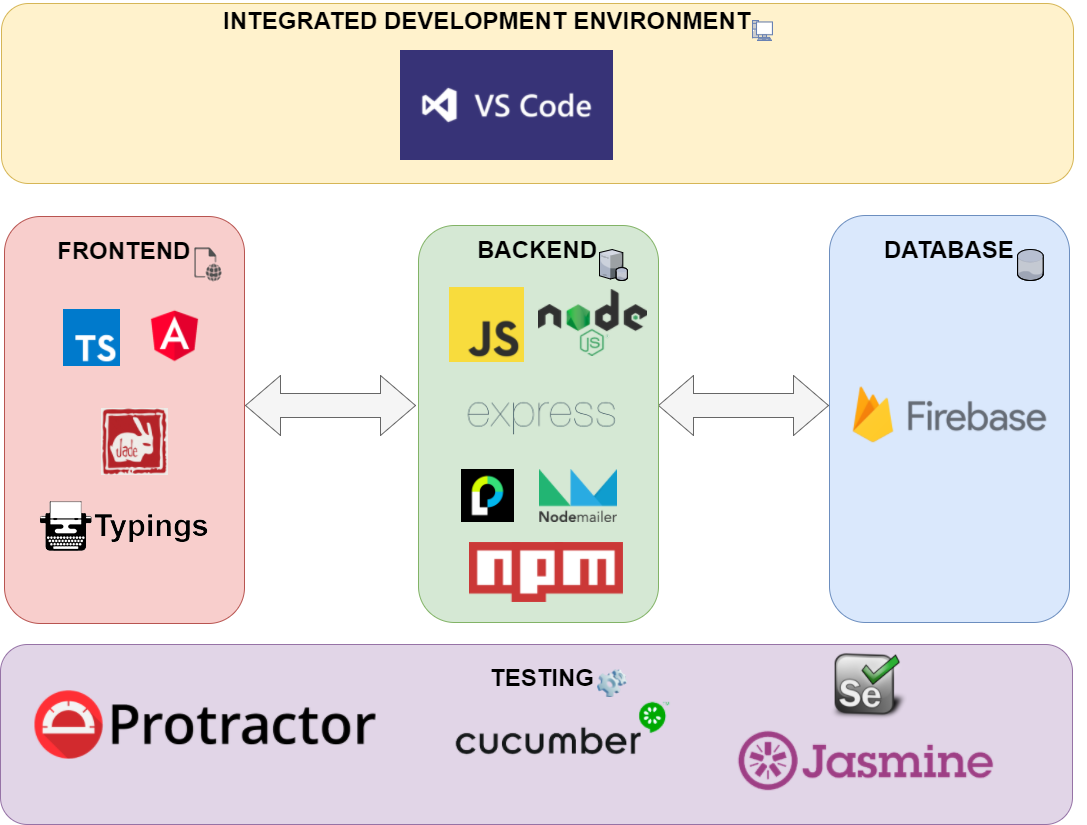
\includegraphics[totalheight=8cm]{resumenTecnologias/Resumen_Tecnolog_as_de_Desarrollo.png}
\caption{Resumen Tecnologías de Desarrollo}
\end{figure}
\vspace{-5mm}

\pagebreak
\subsection{Resumen Tecnologías de planificación y gestión del proyecto}

Las tecnologías que se han usado para generar la documentación y la gestión del proyecto son las que a continuación se muestra, mostrando gráficamente en que se centran cada una de ellas.

\begin{figure}[H]
\centering
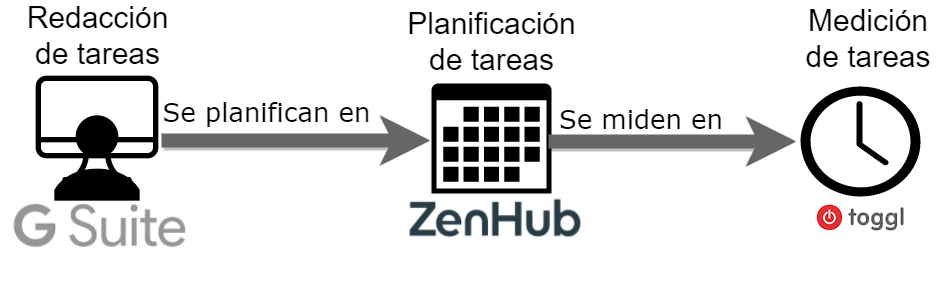
\includegraphics[totalheight=4cm]{resumenTecnologias/Resumen_Tecnolog_as_de_Planificaci_n.png}
\caption{Resumen Tecnologías de planificación y gestión del proyecto}
\end{figure}

\pagebreak
\subsection{Resumen Tecnologías de gestión del código, integración y despliegue continuo}

Éstas tecnologías se encuentran todas en la ``nube'' por lo que sus resultados se encuentran al alcance de cualquier usuario que desea revisarlos, es por ello la representación que se le ha dado en éste apartado.

\begin{figure}[H]
\centering
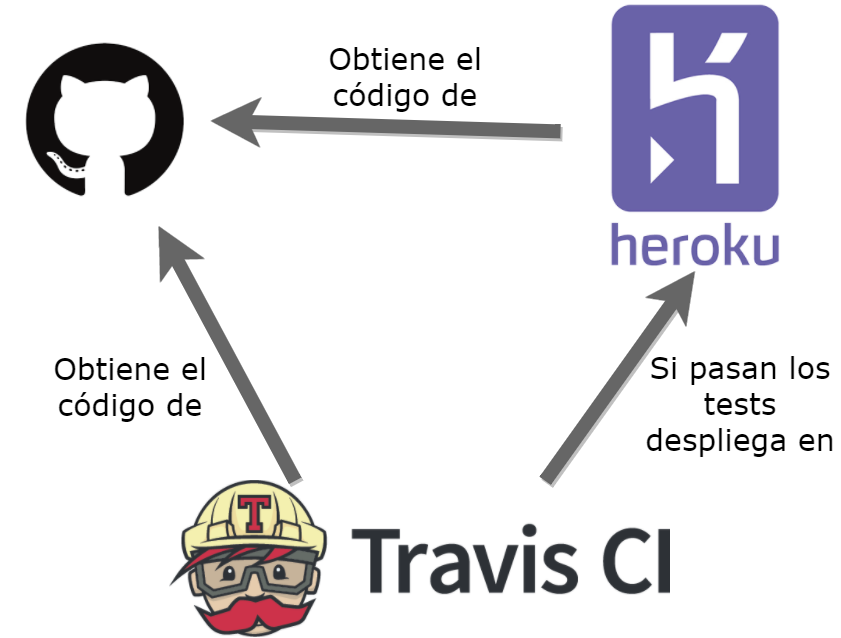
\includegraphics[totalheight=8cm]{resumenTecnologias/Resumen_Tecnolog_as_de_Integraciones.png}
\caption{Resumen Tecnologías de gestión del código, integración y despliegue continuo}
\end{figure}

% 3. Análisis y Diseño: (Mockups, HU, ...)
\chapter{Análisis y Diseño}

Dividiremos el capítulo en secciones con los distintos diagramas que constituyen el análisis y el diseño de la aplicación. Mostraremos además en éste capítulo los mockups del proyecto, cabe destacar que pueden diferir en algunos casos, ya que los dichos mockups se realizaron al comienzo de la aplicación, como se mostrará en el capítulo 4 y la aplicación al seguir un procedimiento de ágil, ha sufrido cambio respecto a los requisitos planteados inicialmente.
\pagebreak

\section{Análisis}

\subsection{Backlog del producto}

A continuación se detallará el Backlog del producto. Éste contiene los requisitos y el Sprint en el que han de ser implementados, cabe destacar que en algunos casos los requisitos se han dividido en ``Fases'', ésto es debido a la estimación seguida, por la que en el caso de estimar un requisito demasiado grande, se divide en trozos más pequeños, con la filosofía ``Divide y vencerás'' y con la finalidad de poder implementar dicho requisito con éxito. 

{\tiny
\setlength{\LTleft}{-20cm plus -1fill}
\setlength{\LTright}{\LTleft}
\begin{center}
\begin{longtable}{| c | M{9.5cm} | M{1.5cm} | M{1cm} | M{1.5cm} |}
\caption[Backlog del Producto]{Backlog del Producto} \label{grid_mlmmh} \\

\hline ID    & Nombre & Iteración / Sprint\\
\endfirsthead

\multicolumn{3}{c}%
{{\bfseries \tablename\ \thetable{} -- continuación de la página anterior}} \\
\hline ID    & Nombre & Iteración / Sprint\\
\hline
\endhead

\hline \multicolumn{2}{|r|}{{Continúa en la página siguiente}} \\ \hline
\endfoot
\endlastfoot
    \hline
    1     & Montaje de la infraestructura & 1 \\
    \hline
    2     & Instalación y elección de las Herramientas & 1 \\
    \hline
    3     & Obtención de datos de Morpheuz & 1 \\
    \hline
    4     & Planificación inicial & 1 \\
    \hline
    5     & Subsistema de login & 2 \\
    \hline
    6     & Almacenamiento de datos en Firebase & 2 \\
    \hline
    7     & Daemon Correo y almacenamiento en Firebase & 2 \\
    \hline
    8     & Procesamiento de datos de Morpheuz & 2 \\
    \hline
    9     & Elegir Framework CSS & 2 \\
    \hline
    10    & Planificación inicial & 2 \\
    \hline
    11    & Estimar puntos de historia & 3 \\
    \hline
    12    & Plantear historias de usuario & 3 \\
    \hline
    13    & Login Back-End & 3 \\
    \hline
    14    & Almacenamiento de login en Firebase & 3 \\
    \hline
    15    & Dummy Chart con movimientos y un componente de Angular & 3 \\
    \hline
    16    & Mockups aplicación & 3 \\
    \hline
    17    & Incluir Angular Material & 3 \\
    \hline
    18    & Imagen Corporativa General & 4 \\
    \hline
    19    & Autenticación al usar Firebase & 4 \\
    \hline
    20    & HU1: Registro en la aplicacón & 4 \\
    \hline
    21    & HU2: Loguearse en la Aplicación & 4 \\
    \hline
    22    & Integrar el proyecto con un CI en la nube & 4 \\
    \hline
    23    & HU3: Acceder a la página principal & 4 \\
    \hline
    24    & HU4: Gestión de datos de perfil y validación & 5 \\
    \hline
    25    & HU5: Representación de datos de firebase en calendario & 5 \\
    \hline
    26    & HU6: Integración de identificación en servicios de 3ºs en los datos de perfil. & 5 \\
    \hline
    27    & HU7: Representación detallada de datos en las gráficas conectada con el calendario. & 5 \\
    \hline
    28    & HU8: Terminar el proceso batch para que procese todos los mails de un usuario. & 5 \\
    \hline
    29    & Integración con la API de Fitbit - Fase 1 & 6 \\
    \hline
    30    & Integración con la API de GoogleFit - Fase 1 & 6 \\
    \hline
    31    & Actualizar historias de usuario & 6 \\
    \hline
    32    & Integración con la API de Fitbit - Fase 2 & 7 \\
    \hline
    33    & Integración con la API de GoogleFit - Fase 2 & 7 \\
    \hline
    34    & Tests - Fase 1 & 7 \\
    \hline
    35    & Tests - Fase 2 & 8 \\
    \hline
    36    & Crear página para que un usuario pueda enlazar sus datos de Morpheuz con la App & 8 \\
    \hline
    37    & Estudiar Integración con la API de Sleep As Android & 8 \\
    \hline
    38    & Añadir opción para recuperar contraseña & 8 \\
    \hline
    39    & Documentar apartado 1 - Introducción & 9 \\
    \hline
    40    & Documentar apartado 2 - Introducción & 9 \\
    \hline
    41    & Documentar apartado 4 - Introducción & 9 \\
    \hline
    42    & Documentar apartado 1 - Revisión & 10 \\
    \hline
    43    & Documentar apartado 2 - Revisión & 10 \\
    \hline
    44    & Documentar apartado 4 - Revisión & 10 \\
    \hline
    45    & Añadir sistema de alertas & 10 \\
    \hline
    46    & Documentar apartado 1 - Finalización & 11 \\
    \hline
    47    & Documentar apartado 2 - Finalización & 11 \\
    \hline
    48    & Documentar apartado 4 - Finalización & 11 \\
    \hline
    49    & Documentar apartado 3 - Introducción & 11 \\
    \hline
    50    & Documentar apartado 7 - Introducción & 11 \\
    \hline
    51	  & Integración con la API de Fitbit - Fase 3 & 11 \\
    \hline
    52	  & Parámetro Alertas	& 12 \\
    \hline
    53	  & Corregir errores en la documentación & 13 \\
    \hline
    54	  & Documentar apartado 6 - Introducción & 13 \\
    \hline
    55	  & Documentar apartado 8 - Introducción & 13 \\
    \hline
    56	  & Corregir errores en la documentación de los nuevos apartados & 14 \\
    \hline
    57	  & Desglose del presupuesto & 14 \\
    \hline
\end{longtable}
\end{center}}

En el capítulo 4, se detallará con mayor información el Backlog que a continuación se muestra, mostrando la estimación en horas y puntos de historia que se estimaron.

\subsection{Historias de Usuario}

Al igual que ocurre con los Mockups mostrados anteriormente, algunas de éstas han sido actualizadas o incluso se han añadido más funcionalidades que las definidas en el diseño de las mismas, ya que éstas se diseñaron al inicio de la aplicación. Sin embargo, como se ha podido comprobar en el Backlog, se han implementado en varios Sprints, por lo que la variación final sufrida respecto a el diseño inicial no ha sido tan notable como en el caso de los Mockups.

Seguidamente pasamos a la definición de las Historias de Usuario:

- HU1:
 
\textbf{ID}:1 \textbf{Nombre}: Registro en la aplicación.\linebreak
\textbf{Descripción}: \textit{\underline{Como}} usuario quiero poder registrarme en la aplicación \textit{\underline{para}} poder acceder a la aplicación al loguearme con los datos del registro.\linebreak
\textbf{Pruebas de aceptación}:
\begin{itemize}
\item Registrarse con los datos correctos y comprobar que efectivamente se realiza con éxito el registro.
\item Revisar que al introducir datos erróneos la aplicación avisa de los fallos en esos datos.
\end{itemize}
 
- HU2:
 
\textbf{ID}:2 \textbf{Nombre}: Loguearse en la aplicación.\linebreak
\textbf{Descripción}: \textit{\underline{Como}} usuario quiero poder loguearme en la aplicación con los datos de mi registro \textit{\underline{para}} poder acceder a mis datos en la aplicación.\linebreak
\textbf{Pruebas de aceptación}:
\begin{itemize}
\item Ingresar los datos de Login correctos y comprobar que se da acceso al usuario a la aplicación.
\item Revisar que al introducir datos erróneos la aplicación avisa de que los datos introducidos no corresponden con los de ningún usuario registrado.
\end{itemize}
 
- HU3:
 
\textbf{ID}:3 \textbf{Nombre}: Acceder a la página principal.\linebreak
\textbf{Descripción}: \textit{\underline{Como}} usuario quiero poder acceder a la página principal de la aplicación \textit{\underline{para}} poder ver mi calendario y seleccionar los días e informes que necesite.\linebreak
\textbf{Pruebas de aceptación}:
\begin{itemize}
\item Comprobar que los datos que se le muestran al usuario son los pertenecientes a ese usuario.
\item Revisar que todos los enlaces funcionan correctamente y que no hay ningún error a la hora de extraer los datos de la base de datos.
\end{itemize}
 
- HU4:
 
\textbf{ID}:4 \textbf{Nombre}: Gestión de datos de perfil y validación.\linebreak
\textbf{Descripción}: \textit{\underline{Como}} usuario quiero que mis datos sean validados y gestionados en el formulario de Login y registro \textit{\underline{para}} verificar que la veracidad de los datos introducidos y ser informado en el caso de que ocurra cualquier error.\linebreak
\textbf{Pruebas de aceptación}:
\begin{itemize}
\item Comprobar que los datos introducidos se procesan con éxito.
\item Revisar la validación de datos al introducir datos erróneos.
\end{itemize}
 
- HU5:
 
\textbf{ID}:5 \textbf{Nombre}: Representación de datos de Firebase en el calendario.\linebreak
\textbf{Descripción}: \textit{\underline{Como}} usuario quiero que ver reflejados que días del calendario contienen información acerca de mis datos de sueño \textit{\underline{para}} acceder a la representación de los datos de ese día.\linebreak
\textbf{Pruebas de aceptación}:
\begin{itemize}
\item Comprobar que los días que contienen datos de sueño se marcan en el calendario como un evento.
\end{itemize}
 


- HU6:
 
\textbf{ID}:6 \textbf{Nombre}: Integración de identificación en servicios de 3ºs en los datos de perfil.\linebreak
\textbf{Descripción}: \textit{\underline{Como}} usuario quiero poder integrar servicios de aplicaciones de terceros en la aplicación \textit{\underline{para}} añadir información de éstos y procesar dicha información.\linebreak
\textbf{Pruebas de aceptación}:
\begin{itemize}
\item Comprobar que la integración con éstos servicios se hace correctamente.
\item Verificar la correcta identificación en dichos servicios.
\end{itemize}
 
 
- HU7:
 
\textbf{ID}:7 \textbf{Nombre}: Acceder a la página de ``Resumen de Sueño'' para un día concreto.\linebreak
\textbf{Descripción}: \textit{\underline{Como}} usuario quiero poder acceder a la página de “Resumen de Sueño” de un día concreto en el que haya registrado datos \textit{\underline{para}} obtener un informe de los distintos valores del sueño relacionado con ese día.\linebreak
\textbf{Pruebas de aceptación}:
\begin{itemize}
\item Comprobar que los datos que se le muestran al usuario son los pertenecientes a ese usuario.
\item Revisar que no hay ningún error a la hora de extraer los datos de la base de datos.
\end{itemize}
 
- HU8:
 
\textbf{ID}:8 \textbf{Nombre}: Terminar el proceso ``batch'' para que procese todos los mails de un usuario.\linebreak
\textbf{Descripción}: \textit{\underline{Como}} usuario quiero que la aplicación cuente con un proceso automático de procesamiento de emails \textit{\underline{para}} que en el caso de que la aplicación se caiga, se procesen los emails pendientes al reiniciarla.\linebreak
\textbf{Pruebas de aceptación}:
\begin{itemize}
\item Comprobar que se procesan los email pendientes correctamente.
\item Verificar que el proceso se ejecuta cada vez que se inicia la aplicación.
\end{itemize}

\subsection{Mockups}

A continuación se mostrarán los Mockups diseñados para la aplicación. Cabe destacar fueron diseñados al principio de la misma y que por tanto han sufrido en algunas ocasiones importantes cambios respecto a la implantación que se ha llevado a cabo. Además, algunas vistas se han añadido con posterioridad a los mismos, por lo que no se encuentran representadas por éstos Mockups, los cuales representan la funcionalidad básica de la aplicación.

\subsubsection{Página de Login y Registro}

\begin{figure}[H]
\centering
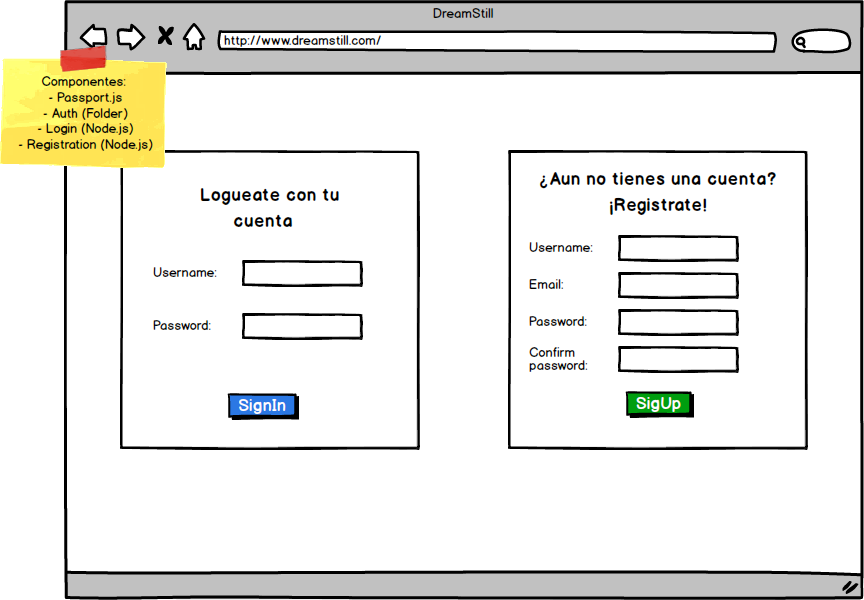
\includegraphics[totalheight=6.5cm]{mockups/LoginPage.png}
\caption{Mockup Página de Login y Registro}
\end{figure}
\par\bigskip 
\noindent

Se desea hacer el acceso al usuario lo más sencillo posible, tanto para los usuarios que ya son de la aplicación, como los que estarían interesados en serlo. Es por ello que el formulario de registro esté al mismo nivel que el de login, de ésta forma, se pretende que el esfuerzo a realizar entre un usuario que ya sea de la aplicación y uno que no lo sea sea similar, animando así a los nuevos usuarios a empezar en la aplicación. 

Además, al estar el formulario de registro visible en todo momento, evitamos ése posible miedo por parte de los usuarios a pensar que tendrán que rellenar una gran cantidad de datos o que el registro se hará pesado, ya que como se puede comprobar, sólo deberá de rellenar algunos datos básicos para acceder a la misma.

\subsubsection{Página principal}

\begin{figure}[H]
\centering
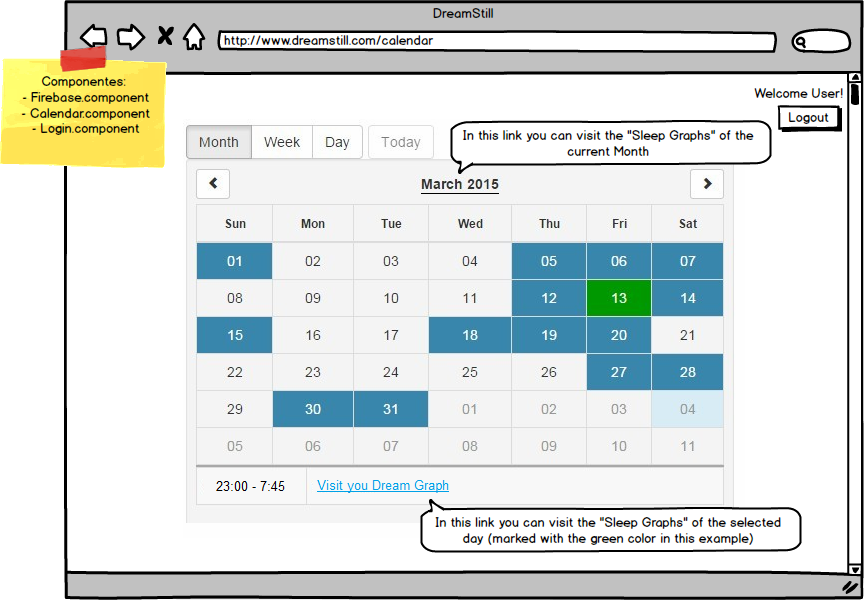
\includegraphics[totalheight=6.5cm]{mockups/CalendarPage.png}
\caption{Mockup Página Principal}
\end{figure}
\par\bigskip 
\noindent

Ésta sería la vista principal que todo usuario que se loguease encontraría nada más entrar. En ella, se encontraría con un calendario en el que se representarían los eventos de sueño y sobre el que podría navegar entre los distintos meses del mismo. Además, el usuario tendrá acceso desde los eventos a la página que contendrá la información de los mismos.

Ésta vista es la que posiblemente haya sufrido uno de los mayores cambios respecto al Mockup planificado. Éstos cambios han sido motivados por el cambio a una interfaz más simple, en la que eliminar posibles menús y aunarlos todos en un mismo botón, que es el que encontramos actualmente en la aplicación y que contiene todas las rutas necesarias para acceder a las distintas partes de la aplicación. De ésta forma, queda una vista mucho más limpia y simple, en la que el usuario podrá centrarse en el calendario y en sus eventos sin distracción alguna.

\subsubsection{Página de Resumen de Sueño Diario}

\begin{figure}[H]
\centering
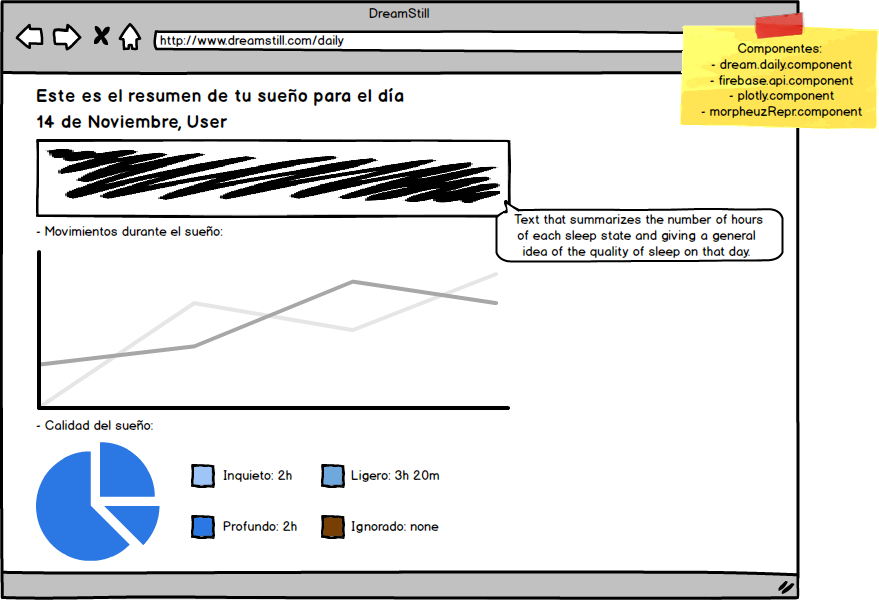
\includegraphics[totalheight=6.5cm]{mockups/DailyDreamPage.png}
\caption{Mockup Página de Resumen de Sueño Diario}
\end{figure}
\par\bigskip 
\noindent

Se compone de dos gráficas. En la primera de ellas el usuario podrá observar como ha sido su estado de sueño en cada intervalo de tiempo de la noche, conociendo cuales fueron los periodos de mayor actividad y en cuales el usuario estuvo prácticamente inmóvil. En la segunda, se muestra de forma resumida la calidad de sueño que se ha tenido, en función de la actividad de ese usuario durante el intervalo de sueño. 

El objetivo de éstas dos gráficas es que el usuario quede informado de su sueño rápidamente y pueda ahondar en más detalles si lo desea interactuando con las mismas.

\pagebreak
\section{Diseño}

\subsection{Diagrama de Componentes}
 
 El siguiente diagrama pretende mostrar cómo está compuesta la aplicación, cuales son sus módulos y cual es la finalidad de cada uno de ellos. Para ello, se definirán la función de cada uno de los módulos por separados, con la intención de que el lector conozca la función de cada uno de ellos.
 
\begin{figure}[H]
\centering
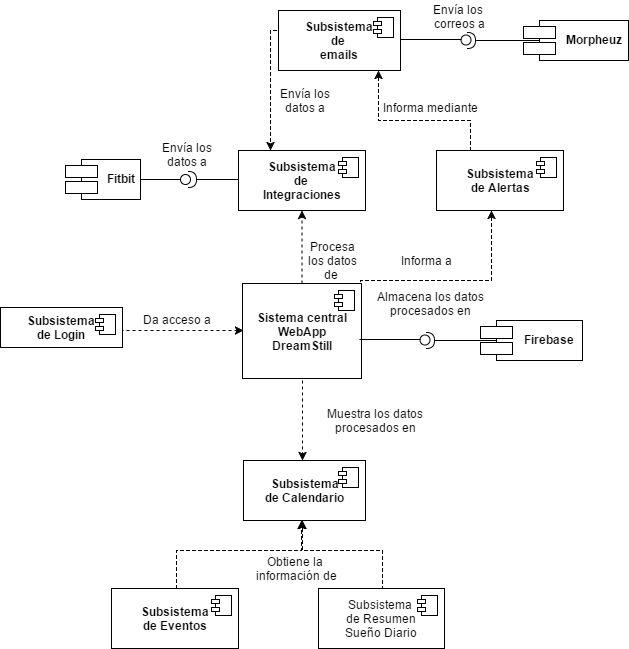
\includegraphics[totalheight=10cm]{diagramas/Diagrama_de_Componentes.png}
\caption{Diagrama de Componentes}
\end{figure}

\begin{itemize}
\item Sistema Central WebApp DreamStill: Es el sistema más importante de la aplicación. Se encarga de obtener y procesar los datos y comunicarlos al resto de subsistemas de la aplicación. En él se encontrarían las funciones más importantes de la aplicación, como la comunicación entre el Subsistema de Integraciones y Firebase o entre éste y el Subsistema de Calendario.
\item Subsistema de Integraciones: Es el subsistema encargado de abstraer al Sistema Central de las distintas integraciones que se añadan a la aplicación, gracias a éste subsistema, a pesar de las distintas integraciones que se realicen, todas serán iguales a instancias del Sistema Central. Por tanto, es necesario que en éste Subsistema se haga un tratado de los datos de las distintas APIs para procesarlos y homogeneizarlos.
\item Subsistema de emails: Es el subsistema encargado de realizar las distintas funciones de correo existentes en la aplicación. Entre ellas se encuentran la lectura de los correos enviados por los usuarios de Morpheuz con sus datos de sueño a la aplicación, o el envío de correos a los usuarios que han establecido una alerta en el sistema.
\item Subistema de Alertas: Es el subsistema encargado de proporcionar al usuario la opción de crear alertas en el sistema, de tal forma que si se cumple una condición impuesta por el usaurio (como por ejemplo dormir menos de 7 horas durante 3 días consecutivos) éste sea informado sin necesitar de tener que acceder a la aplicación para comprobarlo.
\item Subsistema de Calendario: Es el subsistema encargado de proveer y mostrar el calendario que finalmente el usuario encuentra al entrar en la página principal de la aplicación. Provee las distintas funciones como pueden ser navegar al mes anterior, al siguiente o regresar a la fecha actual.
\item Subsistema de Login: Es el sistema encargado de la autenticación de los usuarios. Se encarga de comprobar a través de la información que le proporciona el Sistema Central las correctas credenciales de los usuario y de dar acceso a los mismos a la aplicación. Además, se encarga del registro de nuevos usuarios y de la recuperación de la contraseña de los mismos.
\item Subsistema de Eventos Calendario: Es el subsistema encargado de proveer los eventos que se mostrarán en el calendario de la aplicación, de tal forma que un usuario pueda ver en el calendario en qué días tiene eventos de sueño.
\item Subsistema de Vista Resumen Sueño Diario: Es la vista encargada de mostrar los datos representados gráficamente de una etapa de sueño concreta. De ésta forma, un usuario puede acceder visualmente a éstos datos y obtener reflexiones interesantes de los mismos.
\item Firebase: Es el sistema encargado de comunicarse, leer y almacenar todos los datos en Firebase, nuestra base de datos.
\item Fitbit: Es el subsistema encargado de obtener los datos de Fitbit y transmitirlos al Subsistema de Integraciones para que los procese.
\item Morpheuz: Es el subsistema encargado de controlar las cuentas de Morpheuz de los usuarios y enviar los correos con los datos necesarios al Subsistema de email.
\end{itemize}

\subsection{Diagrama de Despliegue}

Describe la estructura a nivel de hardware de nuestra aplicación. Pretende mostrar de manera gráfica la estructuración de la aplicación dividida en los distintos niveles hardware que la componen. Para nuestro caso concreto estará estructurado en tres niveles.

\begin{figure}[H]
\centering
\includegraphics[totalheight=6cm]{diagramas/Diagrama_de_Despliegue.png}
\caption{Diagrama de Despliegue}
\end{figure}

El primero de ellos, pertenece a la parte del cliente. El entorno de ejecución será para nuestro caso cualquier dispositivo con acceso a la aplicación web, éste a su vez ejecutará el contenido de nuestra aplicación perteneciente al lado del cliente, y provocará que se ejecuten los contenidos necesarios del servidor para poder realizar acciones en nuestra aplicación.

Por otro lado, tenemos la parte del servidor. Para nuestro caso concreto, se alojará en los servidores de Heroku que es donde está alojado nuestra aplicación, y el entorno de ejecución será Docker, el cual gracias a sus contenedores provee mayor escalabilidad en la aplicación. Para poder ejecutar el contenido y las funcionalidades de nuestra aplicación, implementaremos la interfaz de Fitbit y la lectura de emails de Morpheuz. 

Por último, tenemos la parte de base de datos. Para nuestro caso Firebase, base de datos en tiempo real que nos permitirá tener nuestros datos en la ``nube'' y tenerlos actualizados de manera continua, además de ofrecernos la posibilidad de tener un fácil acceso a ellos y además de forma segura.

\pagebreak
\subsection{Diagrama de Capas y Tecnologías}

Se pretende mostrar al lector como están estructuradas las capas de la aplicación. En cada capa se incluirá además las tecnologías que se han usado en cada una de ellas, con la finalidad de diferenciarlas y conocer sus usos.

Para su estructura se ha seguido el modelo Vista/Controlador\cite{18}, el cual se divide en tres capas. La primera de ellas, la de persistencia de datos, en la que se sitúa el sistema de almacenamiento de datos y el sistema gestor de almacenamiento de datos si lo hubiera. En la segunda de ellas, se sitúa el controlador, el cual se define como ``el director de orquesta'' ya que orquesta las distintas llamadas al servidor y proporciona las funcionalidades necesarios al resto de capas. En la tercera de ellas, se sitúa la vista, la cual proporciona los datos del lado del cliente, es decir, los datos que se representan en el navegador del usuario, obteniéndolos del controlador.

\begin{figure}[H]
\centering
\includegraphics[totalheight=6cm]{diagramas/Diagrama_de_Capas_y_Tecnolog_as.png}
\caption{Diagrama de Capas y Tecnologías}
\end{figure}

\pagebreak
\subsection{Diagrama UML}

Describe el diagrama de clases (Diagrma UML\cite{14}) seguido en el diseño del esquema de la Base de Datos. A pesar de utilizar Firebase y de ser éste una Base de Datos NoSQL, el cual permite una estructura que puede ser propensa a cambios, se ha seguido una estructura prefijada, ya que así se consigue una correcta gestión de la Base de Datos.

\begin{figure}[H]
\centering
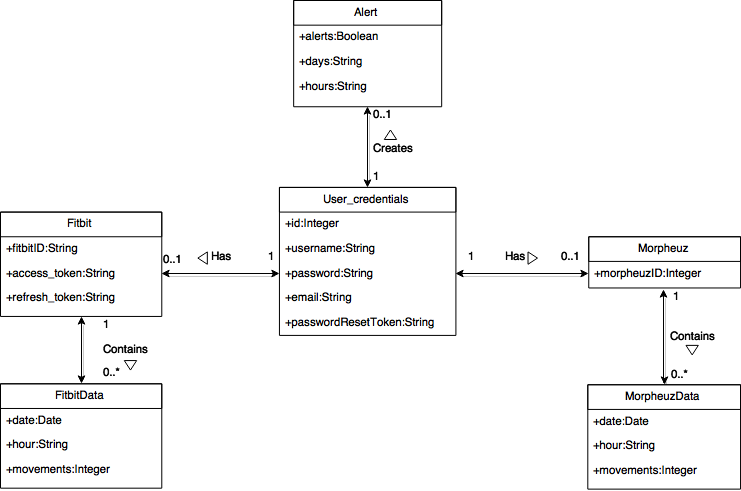
\includegraphics[totalheight=8cm]{diagramas/Diagrama_de_Clases.png}
\caption{Diagrama de Clases}
\end{figure}

Sus clases son las siguientes:

\begin{itemize}
\item User\_Credentials: Clase que almacena los datos básicos de un usuario.
\item Alert: Clase que representa si un ususuario tiene el sistema de alertas activados y los parámetros que ha introducido para dicho sistema.
\item Morpheuz: Clase que almacena el ID de Morpheuz de un usuario y relaciona al mismo con sus datos en dicha aplicación.
\item MorpheuzData: Clase que almacena los datos de movimiento para una hora y fecha concreta obtenidos mediante la aplicación Morpheuz.
\item Fitbit: Clase que almacena los datos necesarios para obtener los datos de la API de Fitbit de un usuario y relaciona al mismo con sus datos en dicha aplicación.
\item FitbitData: Clase que almacena los datos de movimiento para una hora y fecha concreta obtenidos mediante la aplicación Fitbit.

\end{itemize}

% 4. Planificación: (Backlog, Gráficas de Zenhub, Toggl, ...)
\chapter{Planificación}

Para la planificación del proyecto se ha seguido una metodología ágil, en la que cada iteración del proyecto se comprendía en un Sprint. Además, se han desarrollado Historias de Usuario y Mockups, se ha creado un Backlog que contiene todos los requisitos a implementar y se ha creado un fichero de planificación con los requisitos que se implementarán en cada semana durante el transcurso del proyecto.

Para llevar el seguimiento de la planificación y calcular posibles desvíos o estimar la duración de ciertas tareas, se han utilizados herramientas destinadas a éste fin. Éstas herramientas nos han proporcionado datos útiles y han conseguido que se observase de forma clara como avanzaba el proyecto en progreso y en tiempo.

Respecto a los requisitos, al seguir una metodología ágil, partimos de una idea inicial, y los requisitos se fueron detallando y añadiendo en cada una de las reuniones que manteníamos mi tutor y yo, éstas reuniones ocurrían al finalizar cada Sprint y suponían el inicio del siguiente, con unos requisitos definidos para dicho Sprint y a partir de los cuales se realizaba la estimación de los mismos. Se ha seguido una metodología SCRUM\cite{13} adaptada a nuestro proyecto, ésta metodología, es una metodología ágil y consiste en la división de trabajos en ``Sprints'' que son periodos de tiempo en los que se planifican una serie de tareas que implican un incremento en el proyecto\cite{16}, ésta metodología es muy usada en proyectos en los que se definen los requisitos durante el transcurso del proyecto y tiene como beneficios un mayor seguimiento de los entregables por parte del cliente, llamado en ésta metodología ``Product Owner'', el cual tendrá una reunión en cada Sprint para conocer como avanza el proyecto y aprobar las tareas para cada uno de éstos Sprints. Por motivos de tiempo ambas partes no podíamos llevar a cabo una ``Daily meeting'' como se recomienda en dicha metodología, por tanto la metodología de Scrum que hemos seguido sería la que se aprecia en la siguiente figura:

\begin{figure}[H]

\includegraphics[totalheight=5cm]{scrum.png}
\caption{Metodología Scrum}
\end{figure}
\par\bigskip 
\noindent

Respecto a los Sprints, éstos solían ser de dos semanas. Aunque su duración podía variar, dependiendo del momento o fechas que nos encontráramos (casos especiales como Navidad por ejemplo), o de la carga de trabajo que se pretendiese para dicho Sprint. La decisión de ésta duración de dos semanas fue consensuada, ya que llegamos a la conclusión que era un intervalo de tiempo suficientemente amplio como para realizar una buena iteración de cambios pero no tan amplio como para que el proyecto no avanzase a la velocidad que debiera al no poder estimar o corregir a tiempo los errores en la planificación.

El Backlog, ha sido el documento que se incrementaba al final de cada reunión, ya que en el se acordaban y apuntaban los requisitos que se implementarían en el siguiente Sprint, ha habido casos excepcionales en el que algunos requisitos no han llegado a ser implementados debido a que se apuntaron en éste pero por cambios de rumbo en la aplicación o por la re-estructuración de ésta no han llegado a tal implementación. Sin embargo, éstos han sido casos aislados, lo habitual es concretar unos requisitos en la reunión, apuntarlos en el Backlog y estimarlos posteriormente. Es por ello que en el Backlog como mostraremos a continuación, se muestran todas los incrementos que ha sufrido el proyecto junto con el Sprint en el que se han producido y los puntos de historia que se le estimaron.

{\tiny
\setlength{\LTleft}{-20cm plus -1fill}
\setlength{\LTright}{\LTleft}
\begin{center}
\begin{longtable}{| c | M{9.5cm} | M{1.5cm} | M{1cm} | M{1.5cm} |}
\caption[Backlog del Producto]{Backlog del Producto} \label{grid_mlmmh} \\

\hline ID    & Nombre & Estimación & Iteración / Sprint & Puntos de historia\\
\endfirsthead

\multicolumn{3}{c}%
{{\bfseries \tablename\ \thetable{} -- continuación de la página anterior}} \\
\hline ID    & Nombre & Estimación & Iteración / Sprint & Puntos de historia\\
\hline
\endhead

\hline \multicolumn{2}{|r|}{{Continúa en la página siguiente}} \\ \hline
\endfoot
\endlastfoot
    \hline
    1     & Montaje de la infraestructura & 10    & 1     & 13 \\
    \hline
    2     & Instalación y elección de las Herramientas & 3     & 1     & 2 \\
    \hline
    3     & Obtención de datos de Morpheuz & 1,5   & 1     & 1 \\
    \hline
    4     & Planificación inicial & 2     & 1     & 1 \\
    \hline
    5     & Subsistema de login & 5     & 2     & 3 \\
    \hline
    6     & Almacenamiento de datos en Firebase & 8     & 2     & 13 \\
    \hline
    7     & Daemon Correo y almacenamiento en Firebase & 10    & 2     & 21 \\
    \hline
    8     & Procesamiento de datos de Morpheuz & 6     & 2     & 5 \\
    \hline
    9     & Elegir Framework CSS & 2,5   & 2     & 1 \\
    \hline
    10    & Planificación inicial & 0,5   & 2     & 1 \\
    \hline
    11    & Estimar puntos de historia & 1,5   & 3     & 2 \\
    \hline
    12    & Plantear historias de usuario & 2     & 3     & 3 \\
    \hline
    13    & Login Back-End & 4     & 3     & 5 \\
    \hline
    14    & Almacenamiento de login en Firebase & 2     & 3     & 5 \\
    \hline
    15    & Dummy Chart con movimientos y un componente de Angular & 8     & 3     & 8 \\
    \hline
    16    & Mockups aplicación & 2     & 3     & 3 \\
    \hline
    17    & Incluir Angular Material & 2     & 3     & 5 \\
    \hline
    18    & Imagen Corporativa General & 5     & 4     & 8 \\
    \hline
    19    & Autenticación al usar Firebase & 4     & 4     & 5 \\
    \hline
    20    & HU1: Registro en la aplicacón & 3     & 4     & 5 \\
    \hline
    21    & HU2: Loguearse en la Aplicación & 1,5   & 4     & 3 \\
    \hline
    22    & Integrar el proyecto con un CI en la nube & 5     & 4     & 13 \\
    \hline
    23    & HU3: Acceder a la página principal & 3,5   & 4     & 5 \\
    \hline
    24    & HU4: Gestión de datos de perfil y validación & 3     & 5     & 5 \\
    \hline
    25    & HU5: Representación de datos de firebase en calendario & 5     & 5     & 8 \\
    \hline
    26    & HU6: Integración de identificación en servicios de 3ºs en los datos de perfil. & 4     & 5     & 8 \\
    \hline
    27    & HU7: Representación detallada de datos en las gráficas conectada con el calendario. & 6     & 5     & 13 \\
    \hline
    28    & HU8: Terminar el proceso batch para que procese todos los mails de un usuario. & 4     & 5     & 8 \\
    \hline
    29    & Integración con la API de Fitbit - Fase 1 & 12    & 6     & 21 \\
    \hline
    30    & Integración con la API de GoogleFit - Fase 1 & 10    & 6     & 21 \\
    \hline
    31    & Actualizar historias de usuario & 1,5   & 6     & 3 \\
    \hline
    32    & Integración con la API de Fitbit - Fase 2 & 7     & 7     & 13 \\
    \hline
    33    & Integración con la API de GoogleFit - Fase 2 & 6     & 7     & 13 \\
    \hline
    34    & Tests - Fase 1 & 15    & 7     & 21 \\
    \hline
    35    & Tests - Fase 2 & 15    & 8     & 21 \\
    \hline
    36    & Crear página para que un usuario pueda enlazar sus datos de Morpheuz con la App & 3     & 8     & 5 \\
    \hline
    37    & Estudiar Integración con la API de Sleep As Android & 5     & 8     & 8 \\
    \hline
    38    & Añadir opción para recuperar contraseña & 8     & 8     & 5 \\
    \hline
    39    & Documentar apartado 1 - Introducción & 7     & 9     & 13 \\
    \hline
    40    & Documentar apartado 2 - Introducción & 10    & 9     & 21 \\
    \hline
    41    & Documentar apartado 4 - Introducción & 6     & 9     & 13 \\
    \hline
    42    & Documentar apartado 1 - Revisión & 4     & 10    & 8 \\
    \hline
    43    & Documentar apartado 2 - Revisión & 2     & 10    & 5 \\
    \hline
    44    & Documentar apartado 4 - Revisión & 4     & 10    & 8 \\
    \hline
    45    & Añadir sistema de alertas & 8     & 10    & 13 \\
    \hline
    46    & Documentar apartado 1 - Finalización & 4     & 11    & 8 \\
    \hline
    47    & Documentar apartado 2 - Finalización & 2     & 11    & 5 \\
    \hline
    48    & Documentar apartado 4 - Finalización & 3     & 11    & 5 \\
    \hline
    49    & Documentar apartado 3 - Introducción & 9     & 11    & 21 \\
    \hline
    50    & Documentar apartado 7 - Introducción & 9     & 11    & 21 \\
    \hline
    51	  & Integración con la API de Fitbit - Fase 3	 & 6	& 11	& 13 \\
    \hline
    52	  & Parámetro Alertas	& 7	& 12	& 8 \\
    \hline
    53	  & Corregir errores en la documentación & 3	& 13	& 5 \\
    \hline
    54	  & Documentar apartado 6 - Introducción	& 9	& 13	& 21 \\
    \hline
    55	  & Documentar apartado 8 - Introducción	& 9	& 13	& 21 \\
    \hline
    56	  & Corregir errores en la documentación de los nuevos apartados & 5 & 14 & 21 \\
    \hline
    57	  & Desglose del presupuesto & 9 & 14 & 13 \\
    \hline
\end{longtable}
\end{center}}

Para la planificación de las semanas que ocurrirían durante la duración del proyecto se creo un documento con la finalidad de almacenar la información sobre la planificación de éstas. Dicho documento consta de 4 columnas, la primera muestra la semana a la que nos referimos indicando la fecha de inicio de la misma. La segunda, muestra lo que se estimó hacer durante esa semana. La tercera columna muestra una planificación inicial que se hizo al principio del proyecto, en la que yo, estimé cuales serían el número de horas que supuse que tendría disponible durante esas semanas. Por último, nos encontramos con una cuarta columna, en la que se muestra el número de horas reales que se le dedicaron al proyecto en ésa semana.

{\tiny
\setlength{\LTleft}{-20cm plus -1fill}
\setlength{\LTright}{\LTleft}
\begin{center}
\begin{longtable}{| M{1.5cm} | M{9.5cm} | M{1.5cm} | M{1cm} | M{1.5cm} |}
\caption[Backlog del Producto]{Backlog del Producto} \label{grid_mlmmh} \\

\hline Semana & Tareas & Previsión & Realidad \\
\endfirsthead

\multicolumn{3}{c}%
{{\bfseries \tablename\ \thetable{} -- continuación de la página anterior}} \\
\hline Semana & Tareas & Previsión & Realidad\\
\hline
\endhead

\hline \multicolumn{2}{|r|}{{Continúa en la página siguiente}} \\ \hline
\endfoot
\endlastfoot
\hline
10-10-2016 & Instalación y Elección de las Herramientas, Planificación inicial & 5,00  & 8,55 \\
\hline
17-10-2016 & Montaje de la infraestructura, Obtención de datos de Morpheuz & 11,50  & 3,70 \\
\hline
24-10-2016 & Planificación inicial, Subsistema de login, Almacenamiento de datos en Firebase & 12,50  & 8,40 \\
\hline
31-10-2016 & Daemon Correo y almacenamiento en Firebase, Procesamiento de datos de Morpheuz, Elegir Framework CSS & 18,50  & 6,40 \\
\hline
07-11-2016 & Estimar puntos de historia, Plantear historias de usuario, Login Back-End, Almacenamiento de login en Firebase & 11,50  & 6,80 \\
\hline
14-11-2016 & Dummy Chart con movimientos y un componente de Angular, Mockups aplicación, Incluir Angular Material & 12,00  & 6,50 \\
\hline
21-11-2016 & Imagen Corporativa General, Autenticación al usar Firebase, HU1: Registro en la aplicacón & 10,00  & 5,14 \\
\hline
28-11-2016 & HU2: Login, Integración con un CI, HU3: Acceder a la página principal & 8,00  & 7,52 \\
\hline
05-12-2016 & Vectorización del logo, HU4: Gestión de datos de perfil y validación, HU5: Representación de datos de Firebase en calendario & 5,00  & 4,75 \\
\hline
12-12-2016 & HU6: Integración de identificación en servicios de 3ºs, HU7: Representación detallada de dato, HU8: Terminar el proceso batch. & 10,00  & 7,25  \\
\hline
19-12-2016 & Actualizar historias de usuario & 8,00  & 1,00 \\
\hline
26-12-2016 & Integración con la API de GoogleFit & 5,00  & 5,45 \\
\hline
02-01-2017 & Integración con la API de Fitbit & 5,00  & 3,00 \\
\hline
09-01-2017 & Finalización de la Integración con las APIs de GoogleFit y Fitbit & 10,00  & 7,40 \\
\hline
16-01-2017 & Preparar tests aplicación y crear test de prueba en la página principal & 12,00  & 11,95 \\
\hline
23-01-2017 & Página Morpheuz & 12,00  & 8,76 \\
\hline
30-01-2017 & Sleep As Android, Tests & 8,00  & 8,94 \\
\hline
06-02-2017 & Añadir opción para recuperar contraseña & 8,00  & 9,73 \\
\hline
13-02-2017 & Documentación apartado 1 & 12,00  & 7,62 \\
\hline
20-02-2017 & Documentación apartado 2 y 4 & 8,00  & 6,04 \\
\hline
27-02-2017 & Revisión apartados 1 y 2 & 8,00  & 8,05 \\
\hline
06-03-2017 & Revisión apartado 4 y sistema de notificaciones & 12,00  & 7,04 \\
\hline
13-03-2017 & Finalizar apartados 1, 2 y 4 & 12,00  & 7,35 \\
\hline
20-03-2017 & Documentación apartados 3 y 7 & 8,00  & 7,09 \\
\hline
27-03-2017 & Integración con la API de Fitbit & 8,00  & 5,60 \\
\hline
03-04-2017 & Parámetro Alertas & 12,00  & 6,48 \\
\hline
10-04-2017 & Parámetro Alertas & 5,00  & 0,27 \\
\hline
17-04-2017 & Corregir errores en la documentación & 8,00  & 3,23 \\
\hline
24-04-2017 & Corregir errores en la documentación & 6,00  & 2,05 \\
\hline
01-05-2017 & Documentación Apartado 6 y 8 & 5,00  & \\
\hline
08-05-2017 & Documentación Apartado 8 & 12,00  & \\
\hline
15-05-2017 & Corregir errores en la documentación de los nuevos apartados & 10,00  & 1,48 \\
\hline
22-05-2017 & Corregir errores en la documentación de los nuevos apartados & 12,00  & 3,57 \\
\hline
29-05-2017 & Desglose del presupuesto & 12,00  & 5,08 \\
\hline
05-06-2017 & Desglose del presupuesto & 8,00  & 1,07 \\
\hline
TOTAL & 240 & 338,00  & 203,93 \\
\hline
\end{longtable}
\end{center}}

Para conocer una información más detallada de en qué actividades se han invertido tiempo en el proyecto, nos hemos valido de los informes de Toggl, los cuales, como se mostrará a continuación, detallan de una forma fidedigna en qué se ha invertido el tiempo durante el transcurso del proyecto.

Estos informes pretenden mostrar de una forma más clara el impacto en tiempo que ha tenido cada tarea del proyecto, y la continuidad a la hora de desarrollar el proyecto, ya que salvo en pocas excepciones, el trabajo ha sido continuado durante las semanas que ha transcurrido el proyecto.

Con el fin de ayudarnos con el desarrollo de la metodología ágil, y dado que como se ha comentado en capítulo anteriores hemos utilizado Github para la gestión del código, se ha usado una extensión del mismo llamado Zenhub, de la que también se habló en capítulos anteriores. Gracias a dicha herramienta hemos contado con un tablero Kanban:

\begin{figure}[H]
\centering
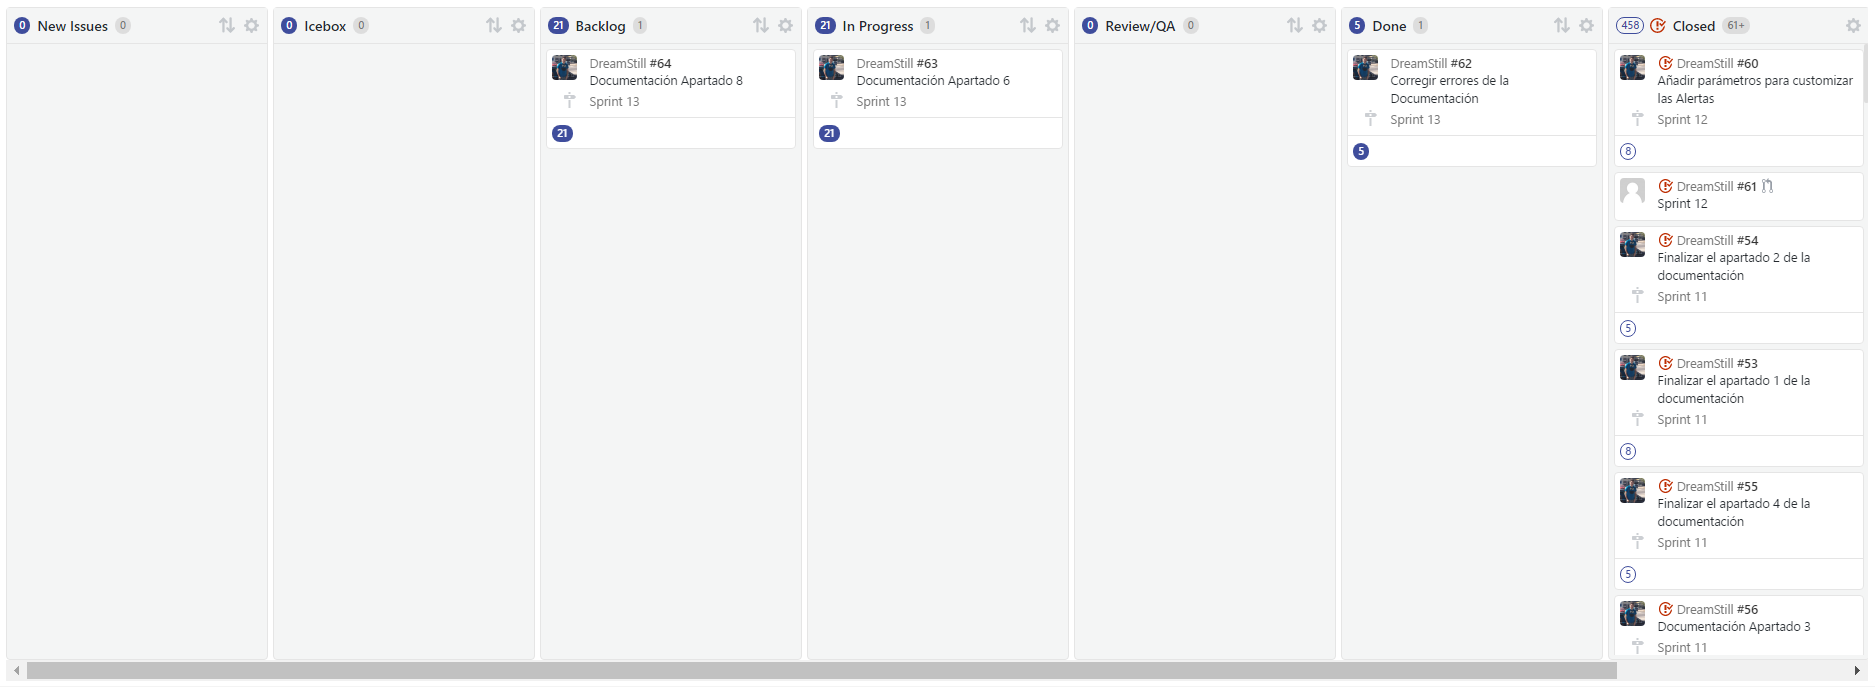
\includegraphics[totalheight=5cm]{kanban.png}
\caption{Tablero Kanban (Zenhub)}
\end{figure}
\par\bigskip 
\noindent

En dicho tablero se apuntan las tareas de cada uno de los Sprints y en el estado en el que se encuentran. En el se han ido registrando los cambios de las tareas (Issues en Github) durante el transcurso del Sprint correspondiente. Además, dicha herramienta, al proporcionarnos una opción para configurar el número de puntos de historia de una tarea, nos realizaba distintos gráficos para conocer el estado del proyecto durante el Sprint correspondiente u otros para ofrecernos una visión global del proyecto. Como se muestra a continuación, durante el transcurso de un Sprint, se realizaban automáticamente gracias a esta herramienta, un gráfico Burndown, el cual mostraba (en gris en el gráfico) un desarrollo ideal de como debían de ir completándose los puntos de historia y a continuación (en azul en el gráfico) mostraba el desarrollo real de dichos puntos de historia en función a como avanzaban las tareas en el tablero Kanban, considerándose como cerradas aquellas tareas que se movían al estado de ``Done'': 

\begin{figure}[H]
\centering
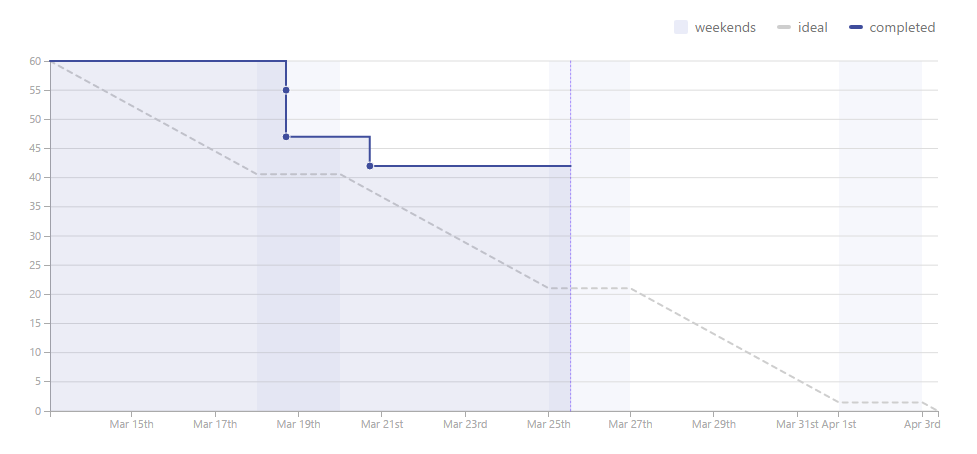
\includegraphics[totalheight=5cm]{zenhub_burndown.png}
\caption{Gráfico Burndown (Zenhub)}
\end{figure}
\par\bigskip 
\noindent

\pagebreak
Además de éstos Burndown, la herramienta Zenhub almacenaba los puntos de historia estimados y completados en cada Sprint, y representaba un gráfico en el que se mostraba el número de puntos de historia completados en cada Sprint y la velocidad media a la que se implementaban.

\begin{figure}[H]
\centering
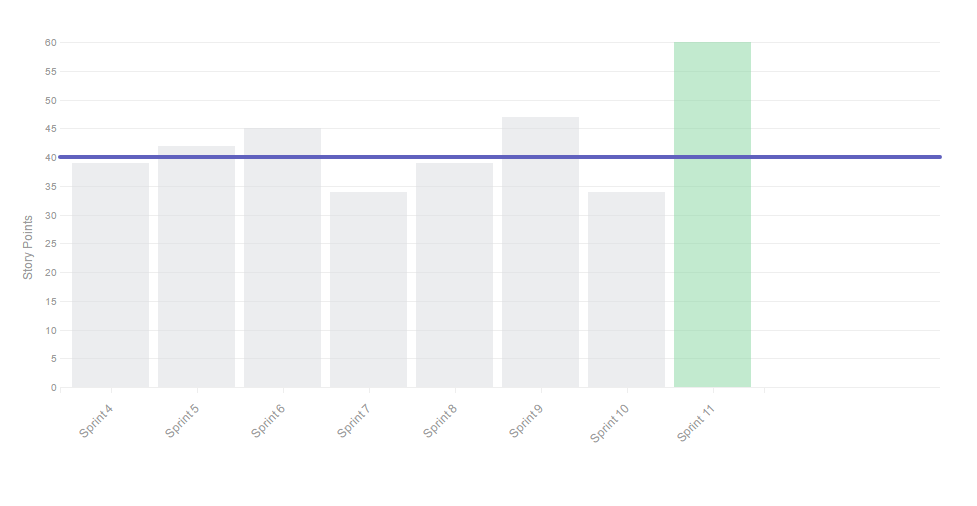
\includegraphics[totalheight=5cm]{zenhub_velocity.png}
\caption{Gráfico Velocity Tracking (Zenhub)}
\end{figure}
\par\bigskip 
\noindent

\section{Detalles de la planificcaión}

En ésta seccion de la planificación se va a detallar el trabajo que se realizó en cada uno de los Sprints a lo largo del proyecto. Además, mostraremos el Burndown de cada uno de los Sprints para analizar cuál fue la desviación respecto a la planificación inicial y se mostrarán los informes de cada uno de los Sprints proporcionados por la herramienta Toggl, gracias a éstos reportes, podremos ver el tiempo que se le dedicó a cada tarea.

\pagebreak
\subsection{Sprint 1}

A lo largo del primer Sprint, se desarrollaron las tareas iniciales del proyecto. Entre ellas, se realizó el montaje de la infraestructura, la cual incluía la creación del proyecto en la plataforma Github, la generación de una aplicación básica y la realización de alguna prueba con Firebase.

Se realizó también la elección y la instalación de las herramientas de desarrollo y la primera obtención de datos de Morpheuz, para comprobar cómo era el formato de éstos y como se podían obtener. Por último en éste primer Sprint, se realizó una planificación inicial, planificando las semanas disponibles para la realización del proyecto y estmiando las horas que se tendrían disponibles en cada una de ellas.

- Burndown:

\begin{figure}[H]
\centering
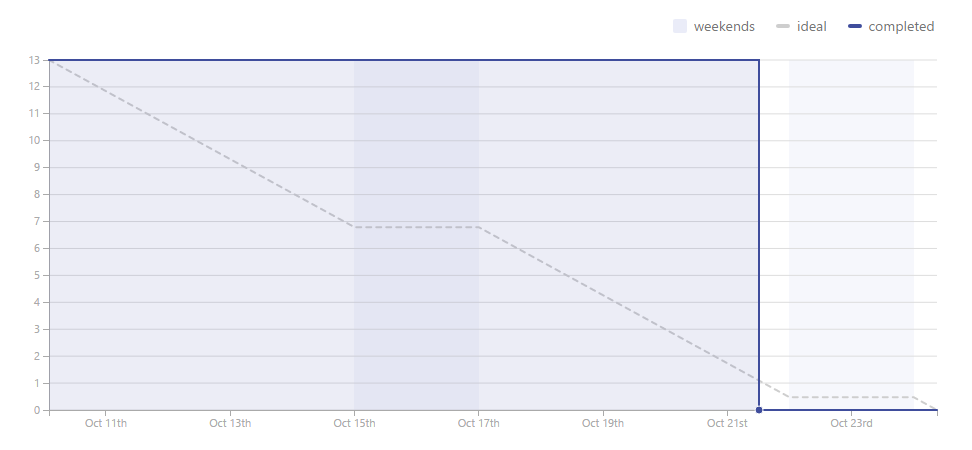
\includegraphics[totalheight=6cm]{burndowns/Sprint1.png}
\caption{Sprint 1}
\end{figure}

- Informe de Toggl:

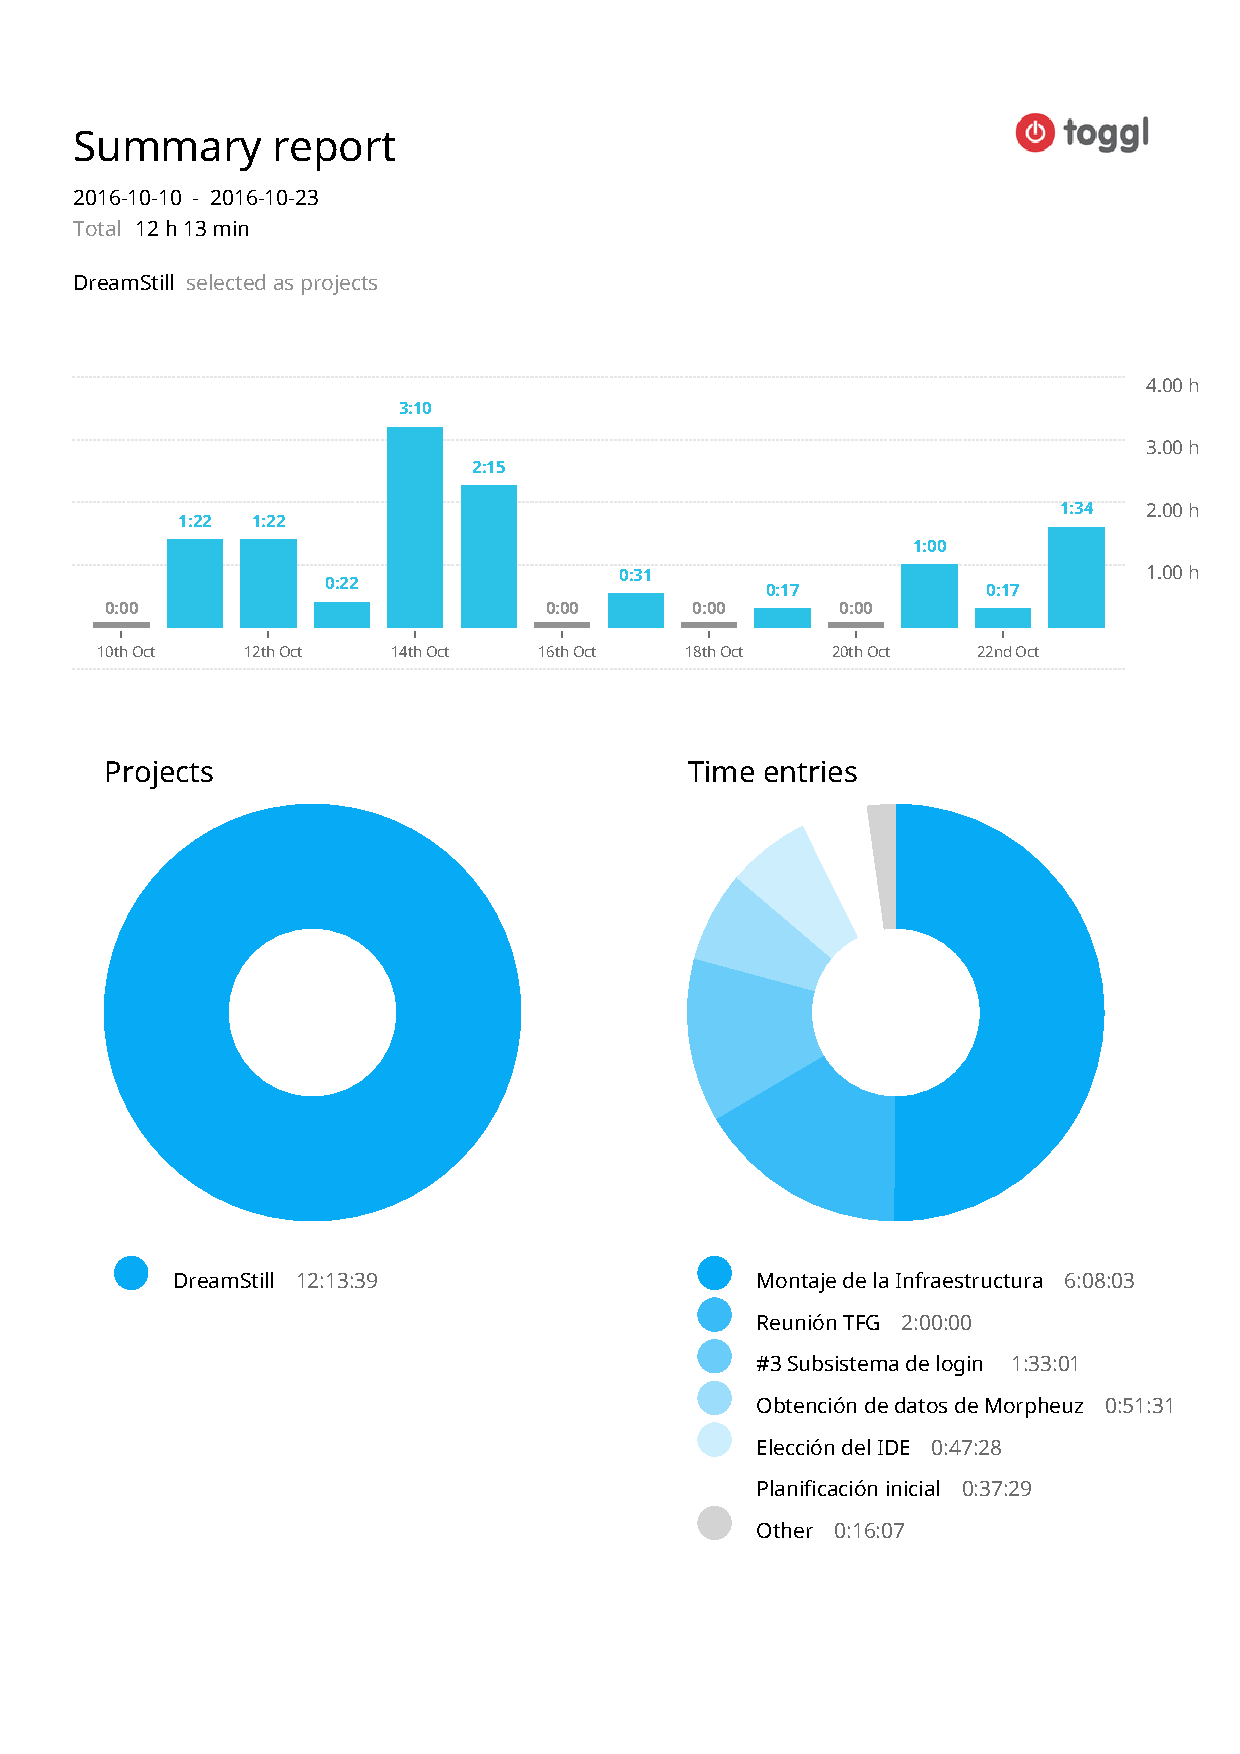
\includepdf[pages={1}]{togglReports/Sprint1.pdf}

\subsection{Sprint 2}

A lo largo del segundo Sprint, se realizaron tareas con la finalidad de obtener la funcionalidad básica del proyecto y comprobar que las tecnologías elegidas para el proyecto eran las adecuadas. Entre éstas tareas se encuentra el subsistema de login, el primer almacenamiento de datos en Firebase y un proceso para comprobar la dirección de correo de la aplicación a la espera de nuevos correos, para obtener los datos de sueño de la aplicación Morpheuz de los usuarios de la aplicación y almacenar dichos datos en Firebase.

Sin embargo, los datos de Morpheuz debían de ser procesados antes de almacenarlos, y también se llevo a cabo éste procesamiento durante el segundo Sprint. Además, se eligió el Framework de CSS usado durante el proyecto y se terminó la planificación inicial, la cual había quedado incompleta en el primer Sprint.

- Burndown:

\begin{figure}[H]
\centering
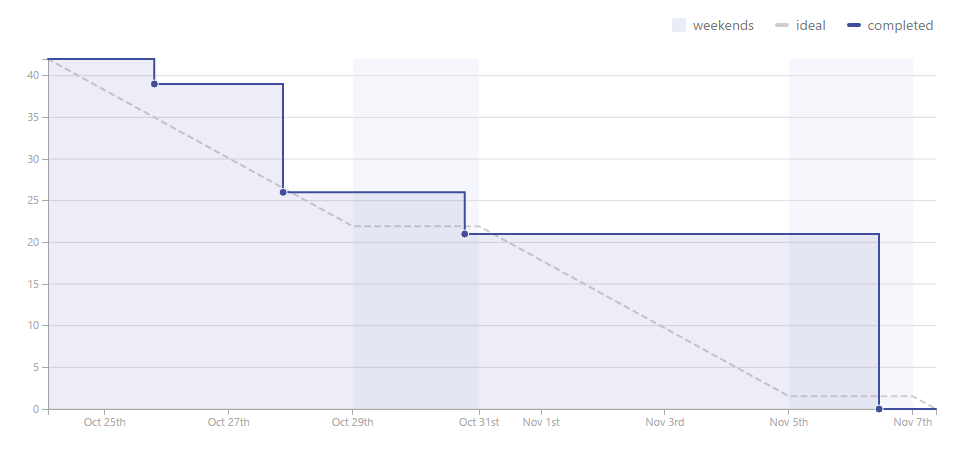
\includegraphics[totalheight=6cm]{burndowns/Sprint2.png}
\caption{Sprint 2}
\end{figure}

- Informe de Toggl:

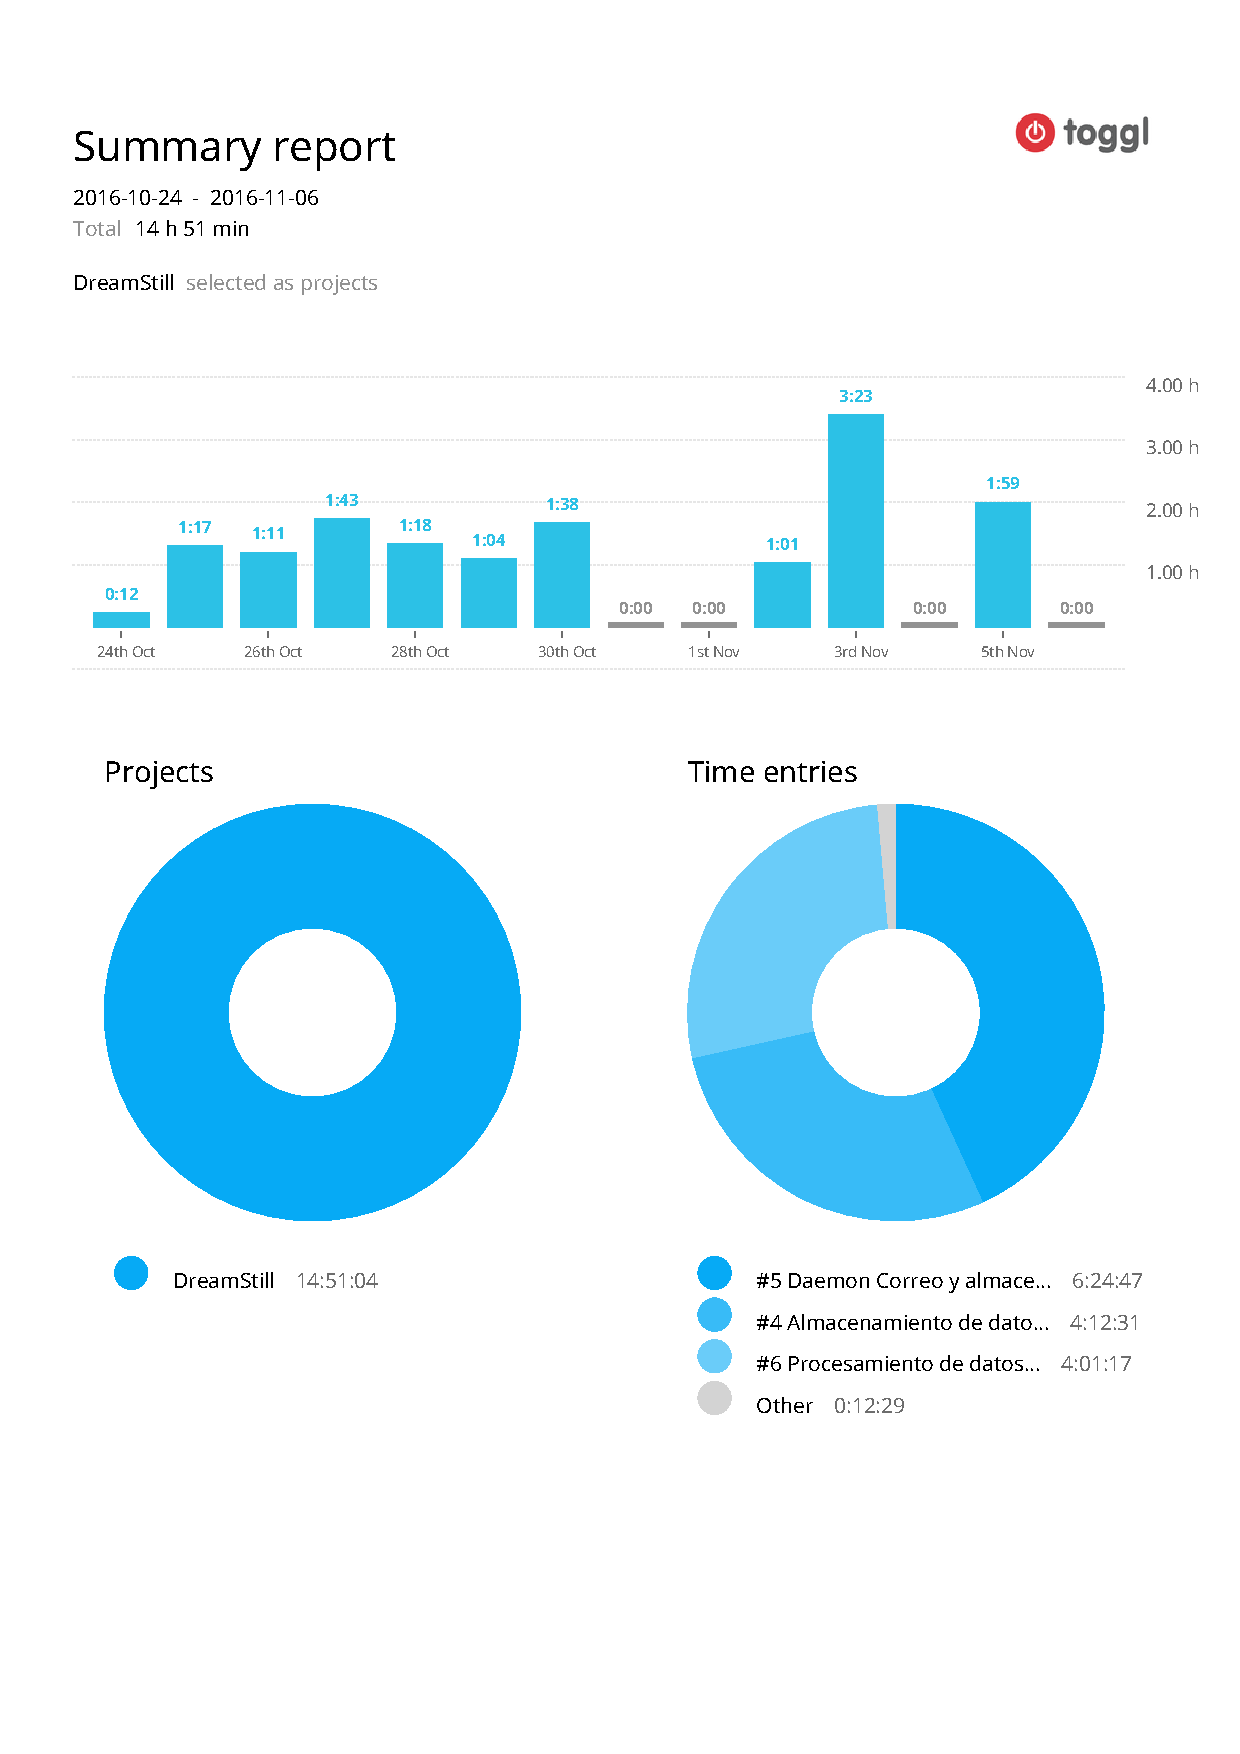
\includepdf[pages={1}]{togglReports/Sprint2.pdf}

\subsection{Sprint 3}

A lo largo del tercer Sprint, se estimó los puntos de historia de las tareas anteriores y de las siguientes en ése esprint y se plantearon las historias de usuario. Además, se realizó la parte de login en el servidor, se conectó dicha parte con Firebase para almacenar los datos de acceso de los usuarios y se creo un primer gráfico representando los datos de Morpheuz. 

Para terminar, en éste Sprint se diseñaron los Mockups y se incluyo el Framework de CSS elegido, que en el caso de nuestro proyecto fue ``Angular Material''.

- Burndown:

\begin{figure}[H]
\centering
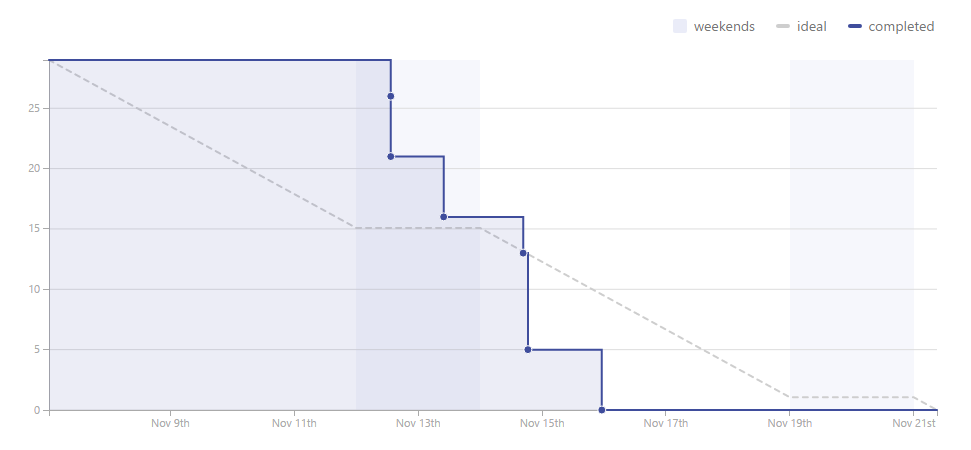
\includegraphics[totalheight=6cm]{burndowns/Sprint3.png}
\caption{Sprint 3}
\end{figure}

- Informe de Toggl:

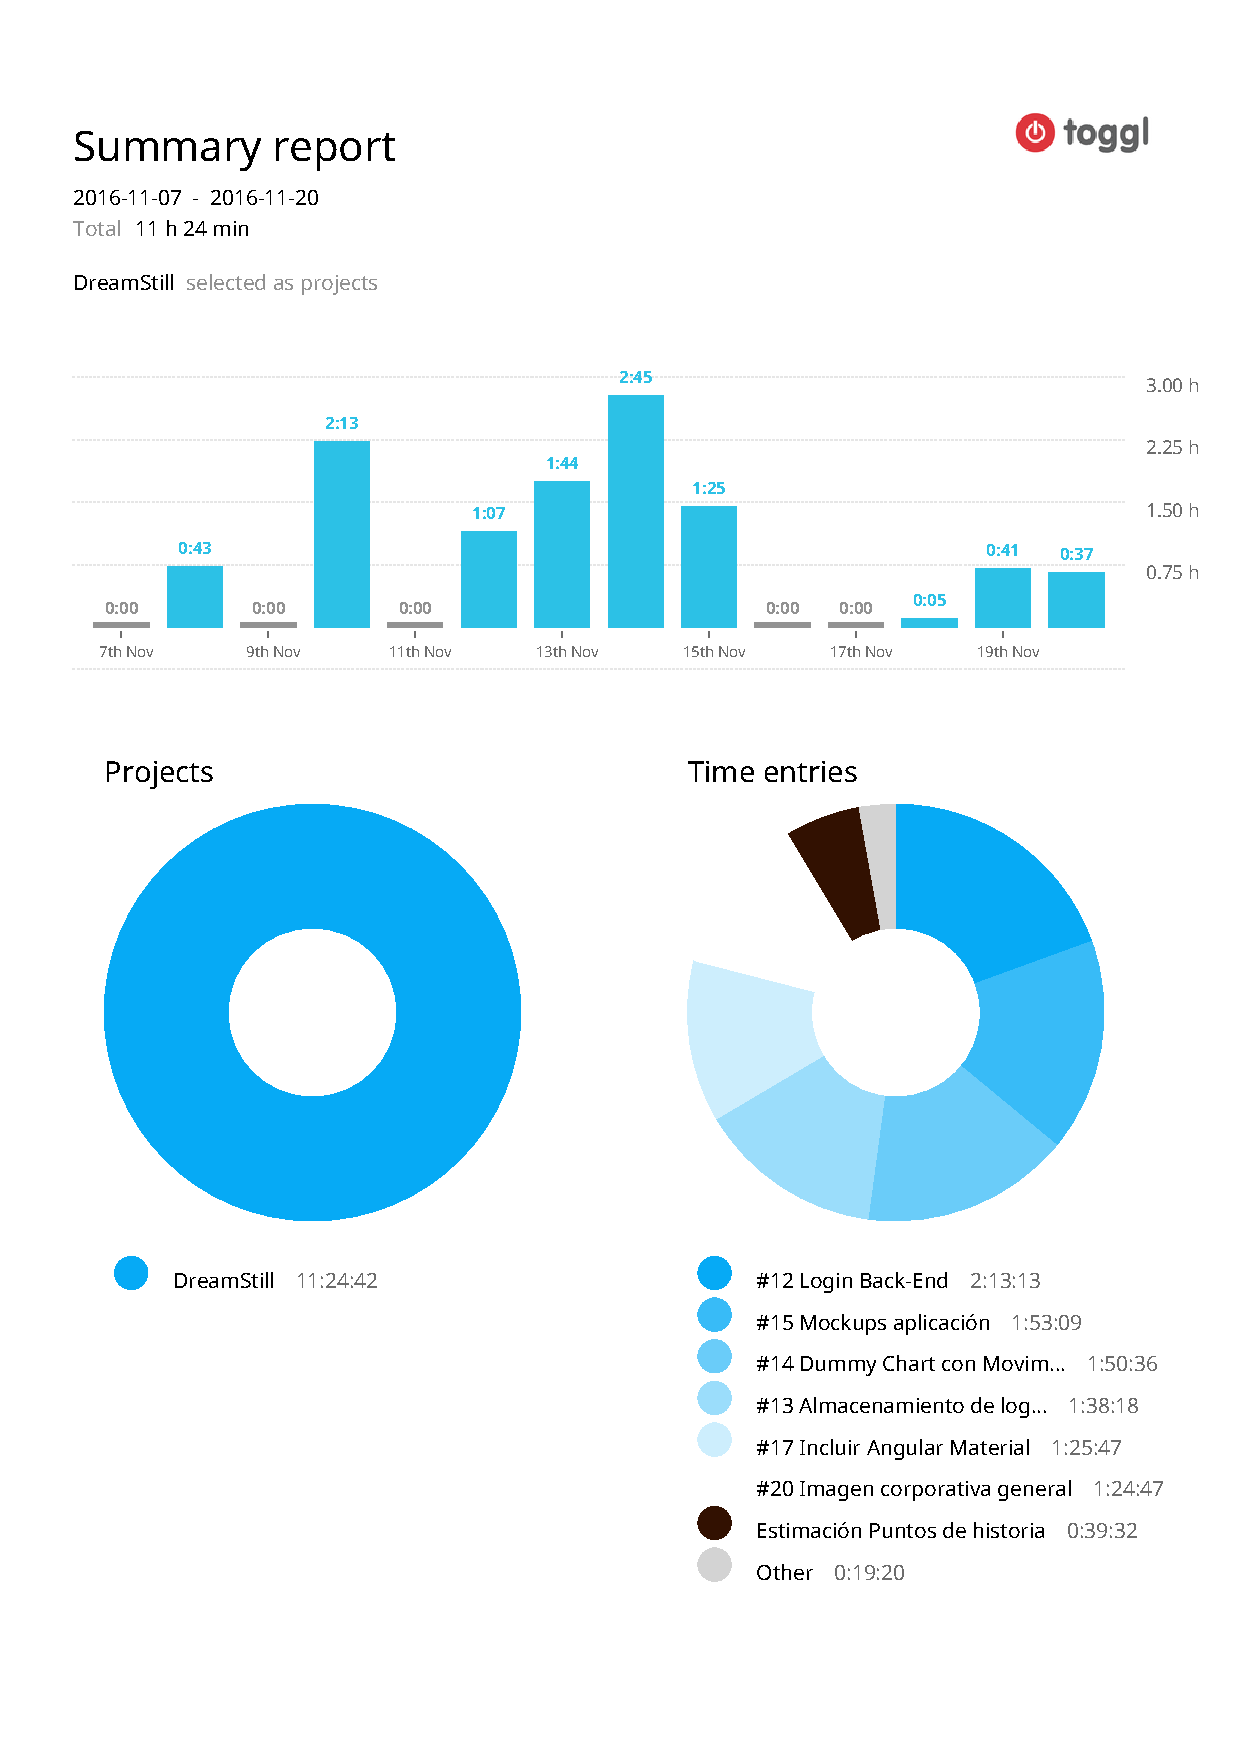
\includepdf[pages={1}]{togglReports/Sprint3.pdf}

\subsection{Sprint 4}

A lo largo del cuarto Sprint, se diseñó la Imagen Corporativa General de la aplicación, se añadió la seguridad a Firebase y se integró el proyecto con Travis. Además, se comenzaron a implementar las primeras historias de usuario, concretamente las tres primeras.

- Burndown:

\begin{figure}[H]
\centering
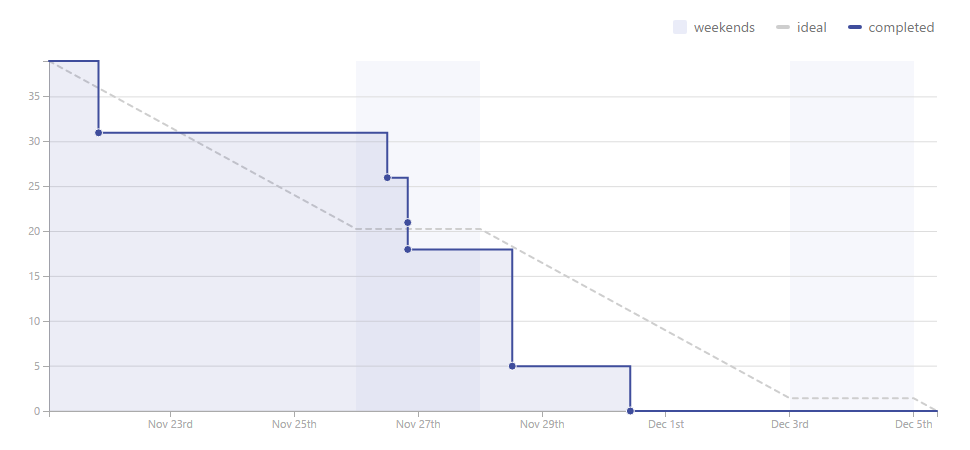
\includegraphics[totalheight=6cm]{burndowns/Sprint4.png}
\caption{Sprint 4}
\end{figure}

- Informe de Toggl:

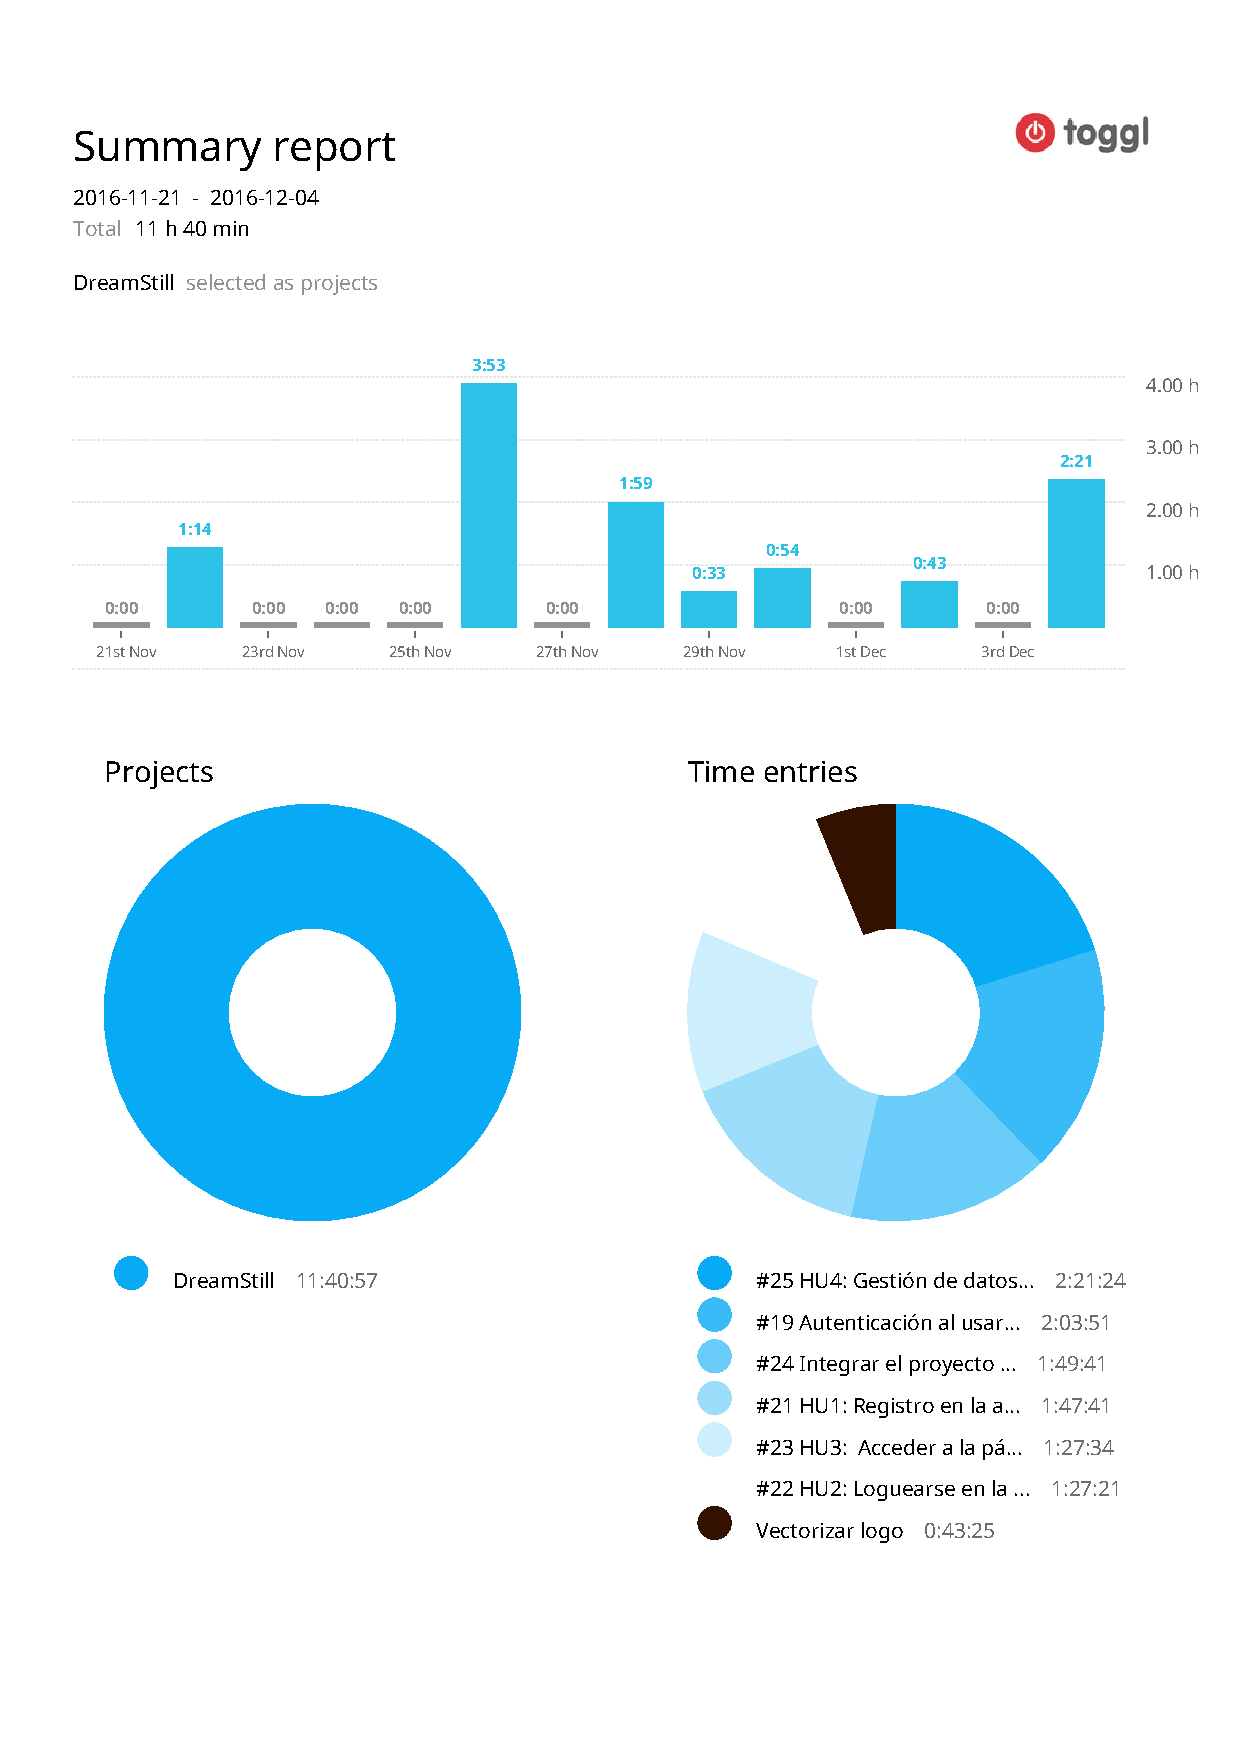
\includepdf[pages={1}]{togglReports/Sprint4.pdf}

\subsection{Sprint 5}

A lo largo del quinto Sprint, se desarrollaron las siguientes 5 historias de usuario definidas en el Sprint 3, es decir, desde la cuarta historia de usuario hasta la octava.

- Burndown:

\begin{figure}[H]
\centering
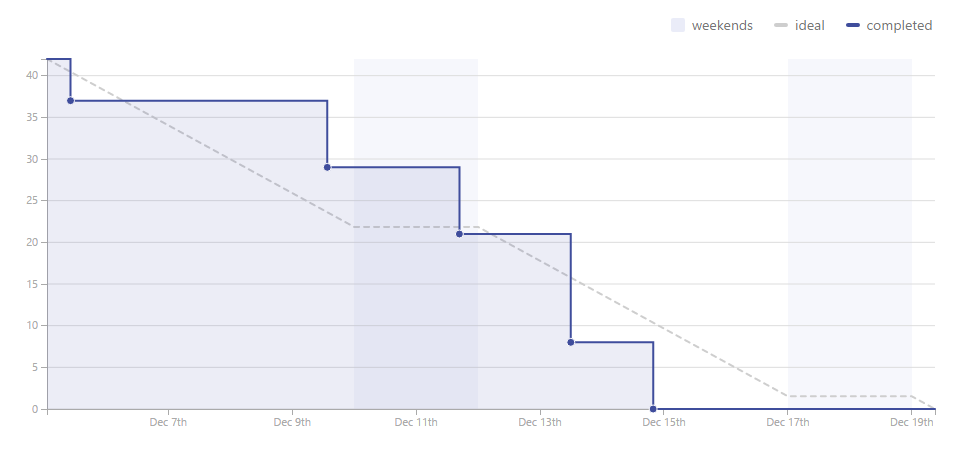
\includegraphics[totalheight=6cm]{burndowns/Sprint5.png}
\caption{Sprint 5}
\end{figure}

- Informe de Toggl:

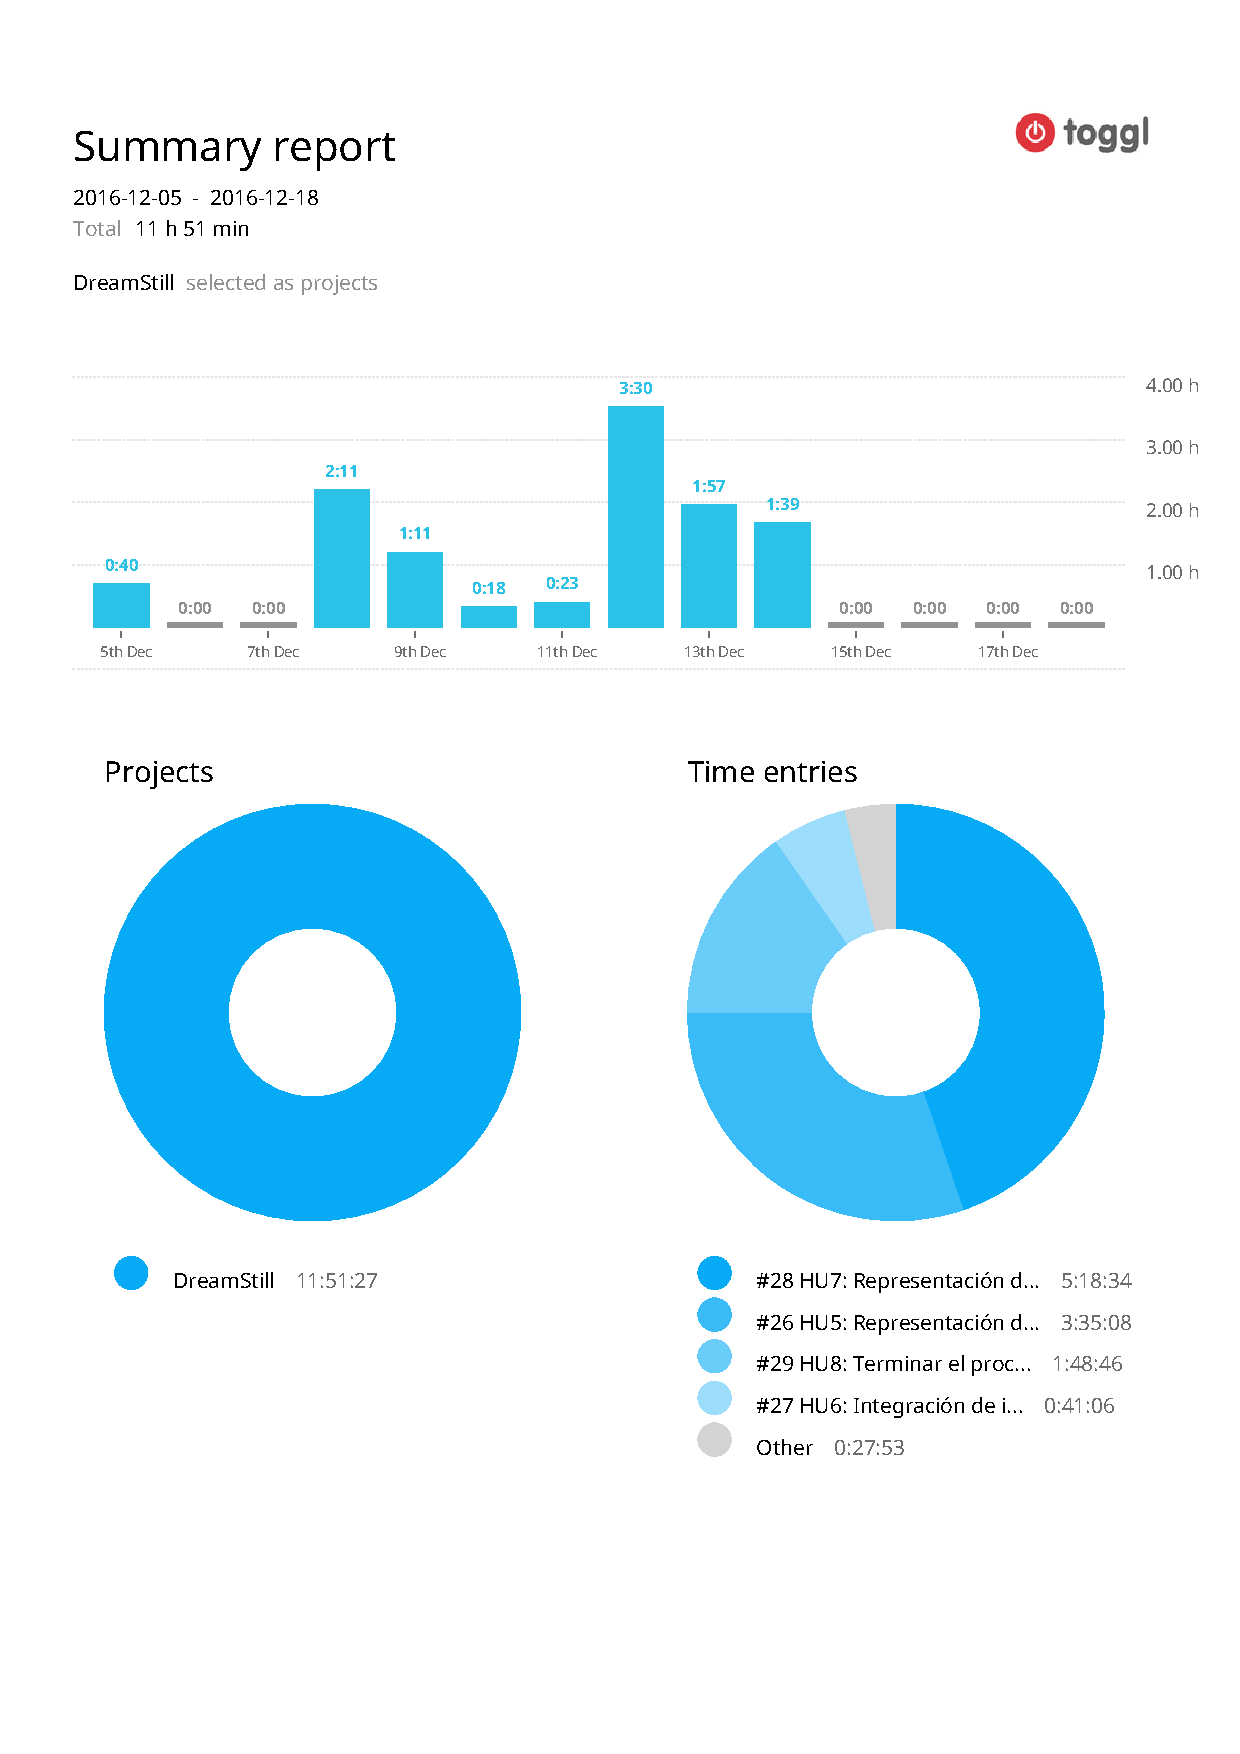
\includepdf[pages={1}]{togglReports/Sprint5.pdf}

\subsection{Sprint 6}

A lo largo del sexto Sprint, se comenzó la primera fase de la integración con las APIs de GoogleFit y Fitbit. Éstas APIs, son tecnologías que ofrecen muchas de las empresas del sector tecnológico actualmente y que permiten a otras aplicaciones obtener datos de sus bases de datos a traves de llamadas realizadas bajo protocolos de Internet. 

Debido a nuevas ideas que surgieron durante la ejecución del presente Sprint, se llevó a cabo una actualización de las historias de usuario anteriormente planteadas.

- Burndown:

\begin{figure}[H]
\centering
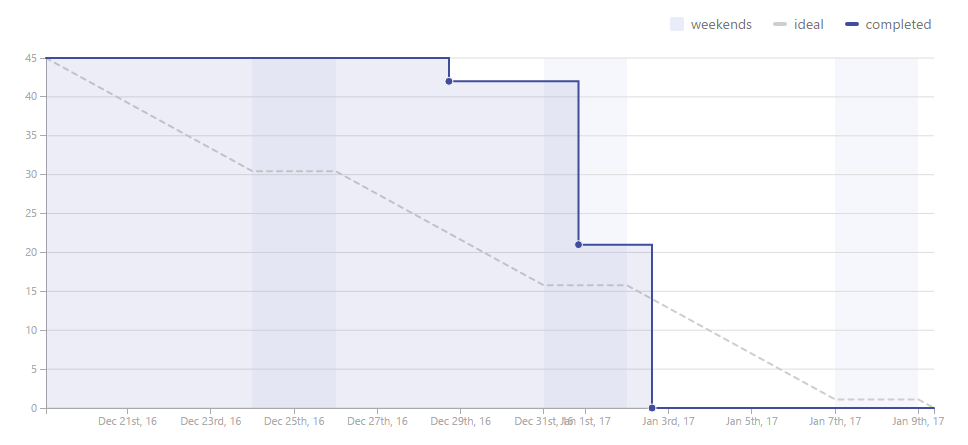
\includegraphics[totalheight=6cm]{burndowns/Sprint6.png}
\caption{Sprint 6}
\end{figure}

- Informe de Toggl:

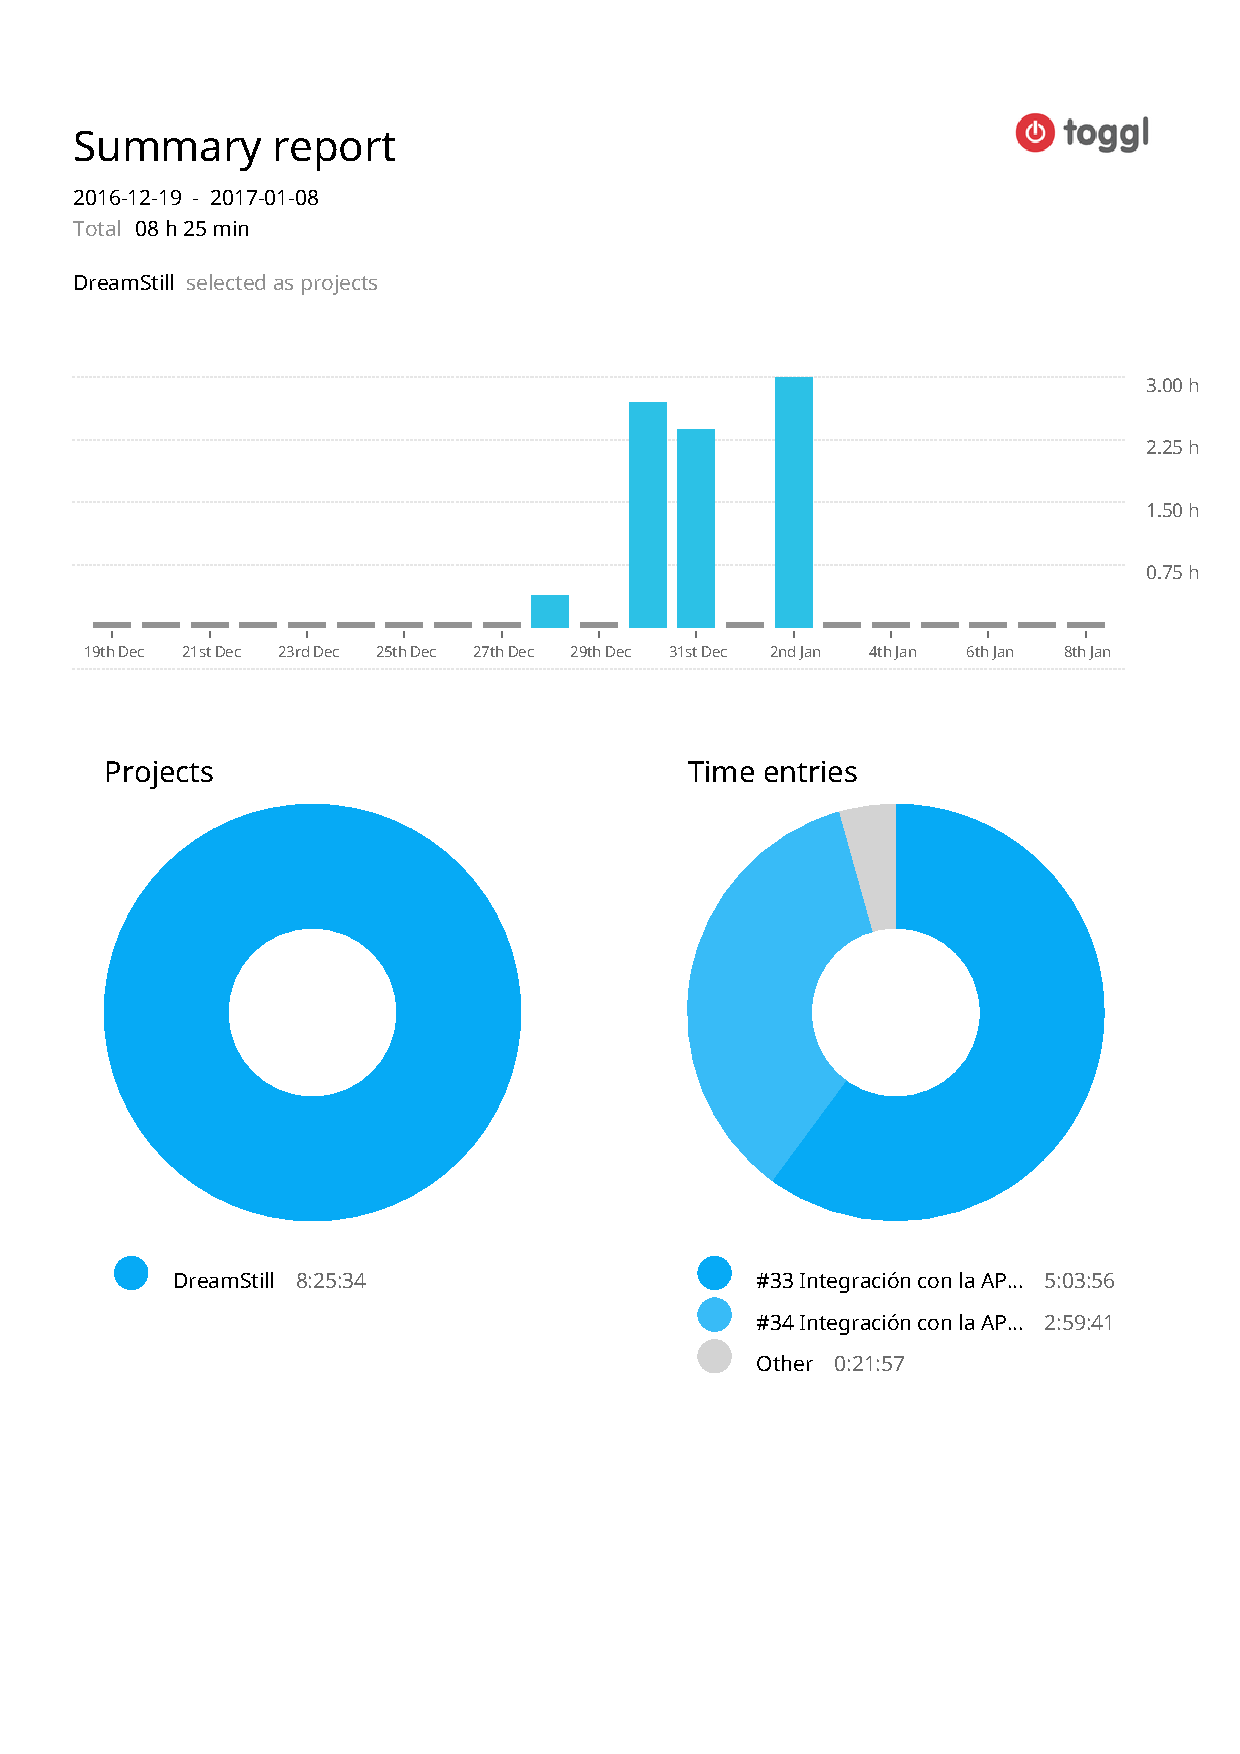
\includepdf[pages={1}]{togglReports/Sprint6.pdf}

\subsection{Sprint 7}

A lo largo del séptimo Sprint, se continuó la fase de integración con las APIs de GoogleFit y Fitbit y se comenzó con los primeros tests funcionales de la aplicación.

- Burndown:

\begin{figure}[H]
\centering
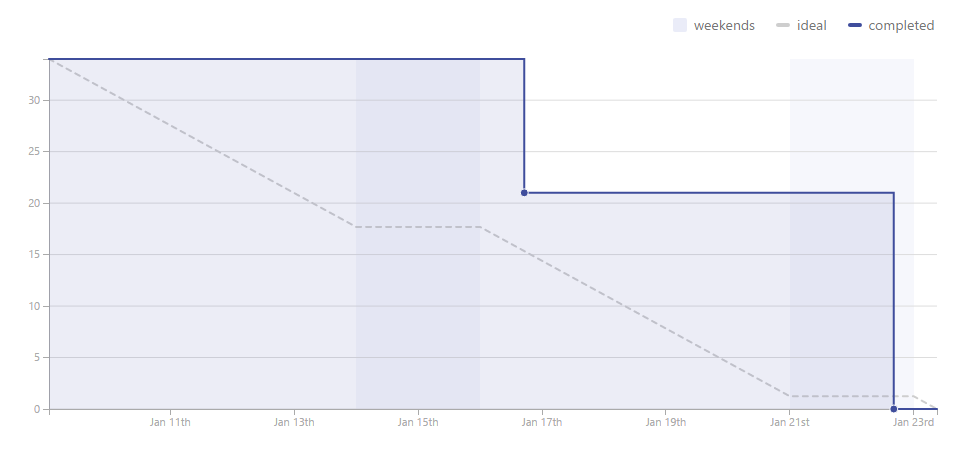
\includegraphics[totalheight=6cm]{burndowns/Sprint7.png}
\caption{Sprint 7}
\end{figure}

- Informe de Toggl:

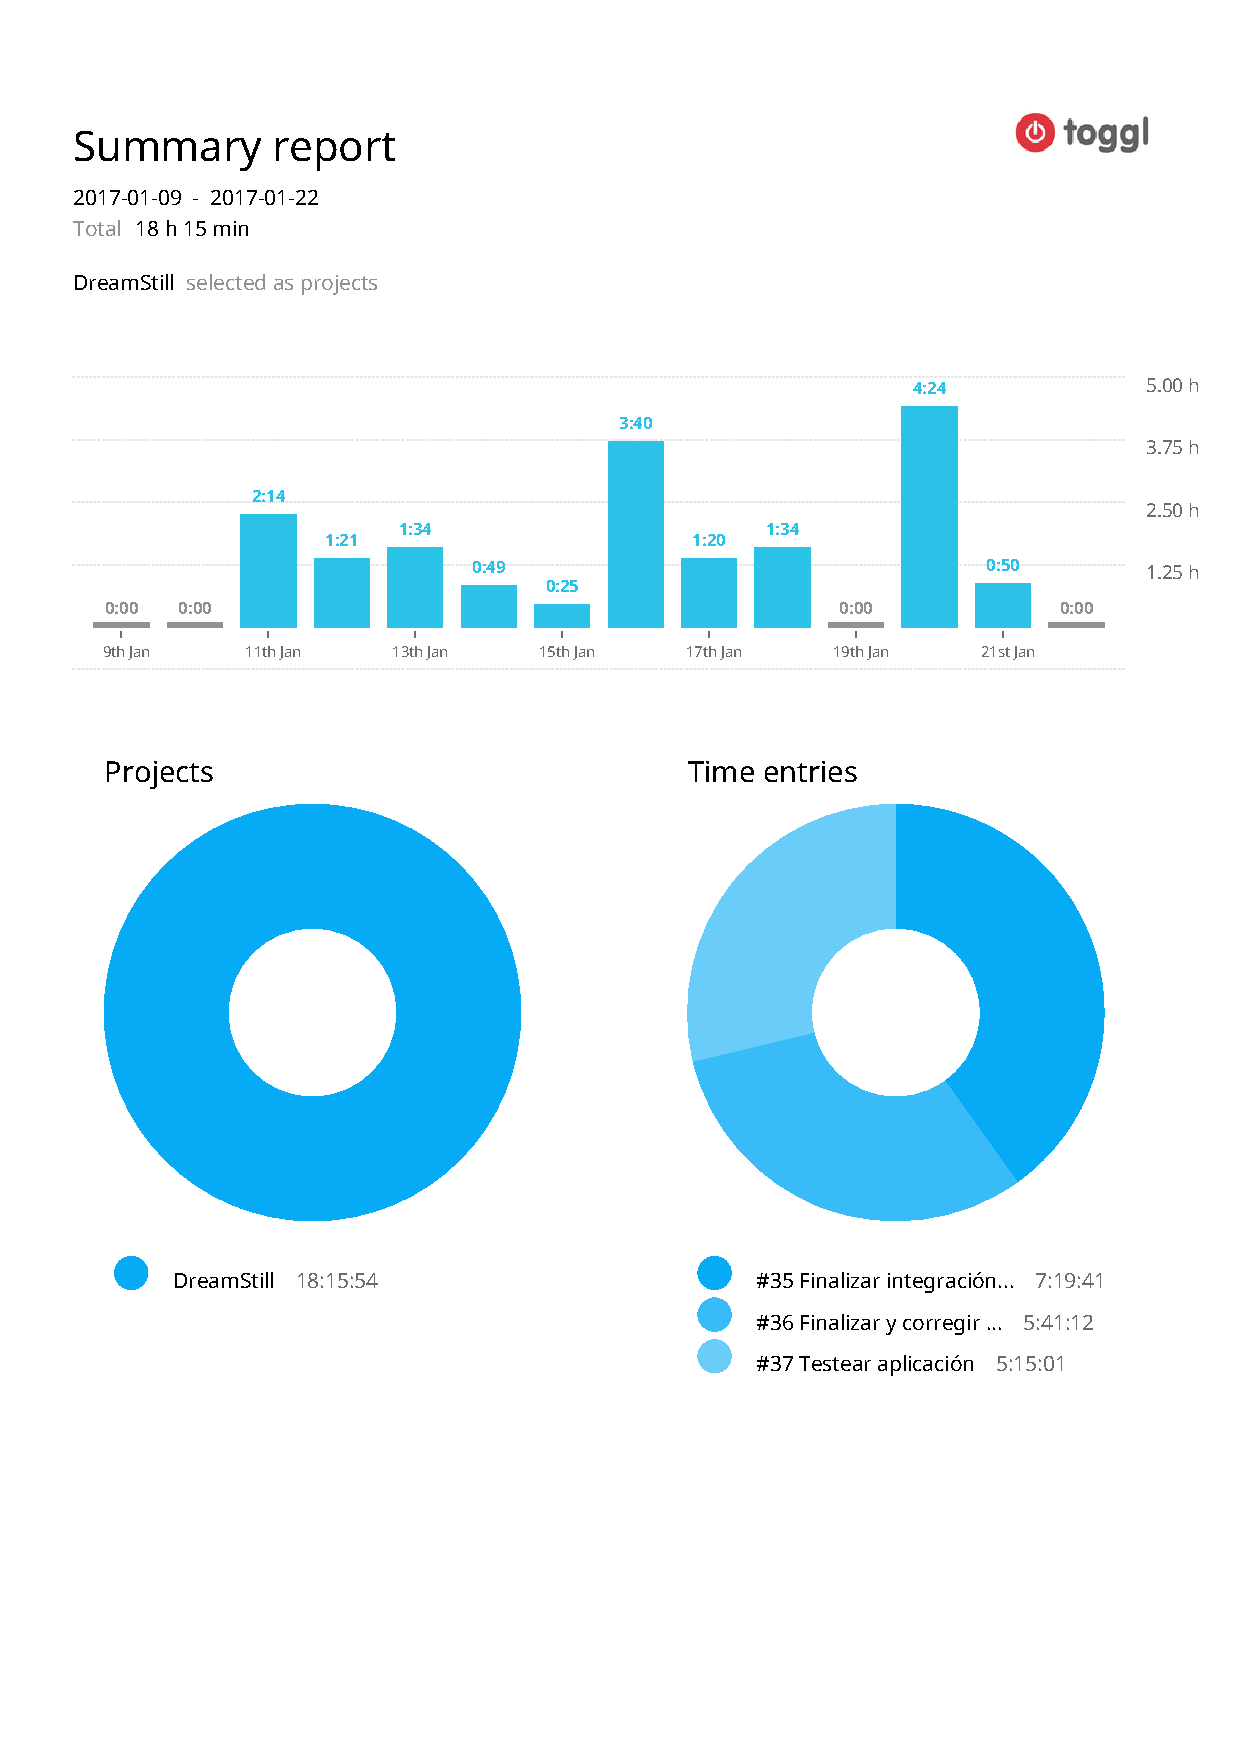
\includepdf[pages={1}]{togglReports/Sprint7.pdf}

\subsection{Sprint 8}

A lo largo del octavo Sprint, se desarrollaron el resto de test funcionales de la aplicación, se creo una página para que los usuarios conocieran los pasos a seguir para enlazar su cuenta de DreamStill con la cuenta de Morpheuz y se estudió la posible integración con la API de Sleep As Android. Respecto a ésta integración, se llego a la conclusión de que no era una buena alternativa a seguir. 

Para terminar, en éste Sprint se añadió la opción de recuperación de contraseñas de la aplicación, para aquellos usuarios que olvidaran su contraseña y no pudieran acceder.

- Burndown:

\begin{figure}[H]
\centering
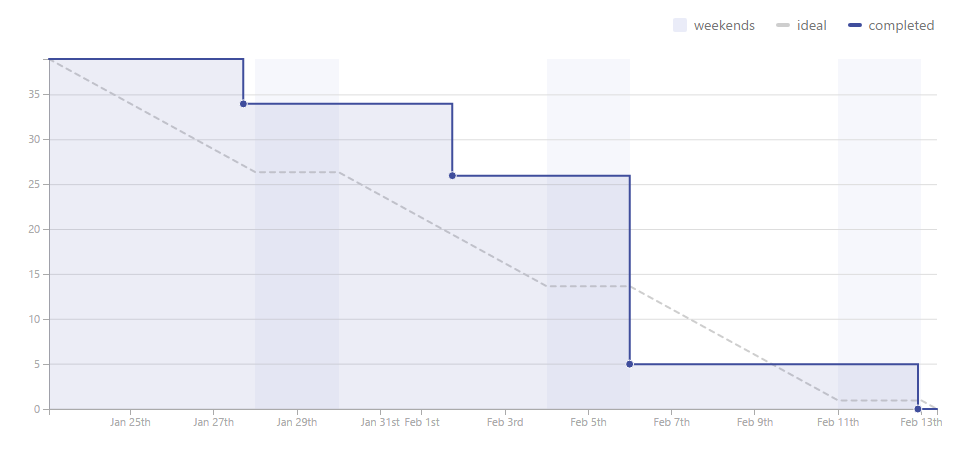
\includegraphics[totalheight=6cm]{burndowns/Sprint8.png}
\caption{Sprint 8}
\end{figure}

- Informe de Toggl:

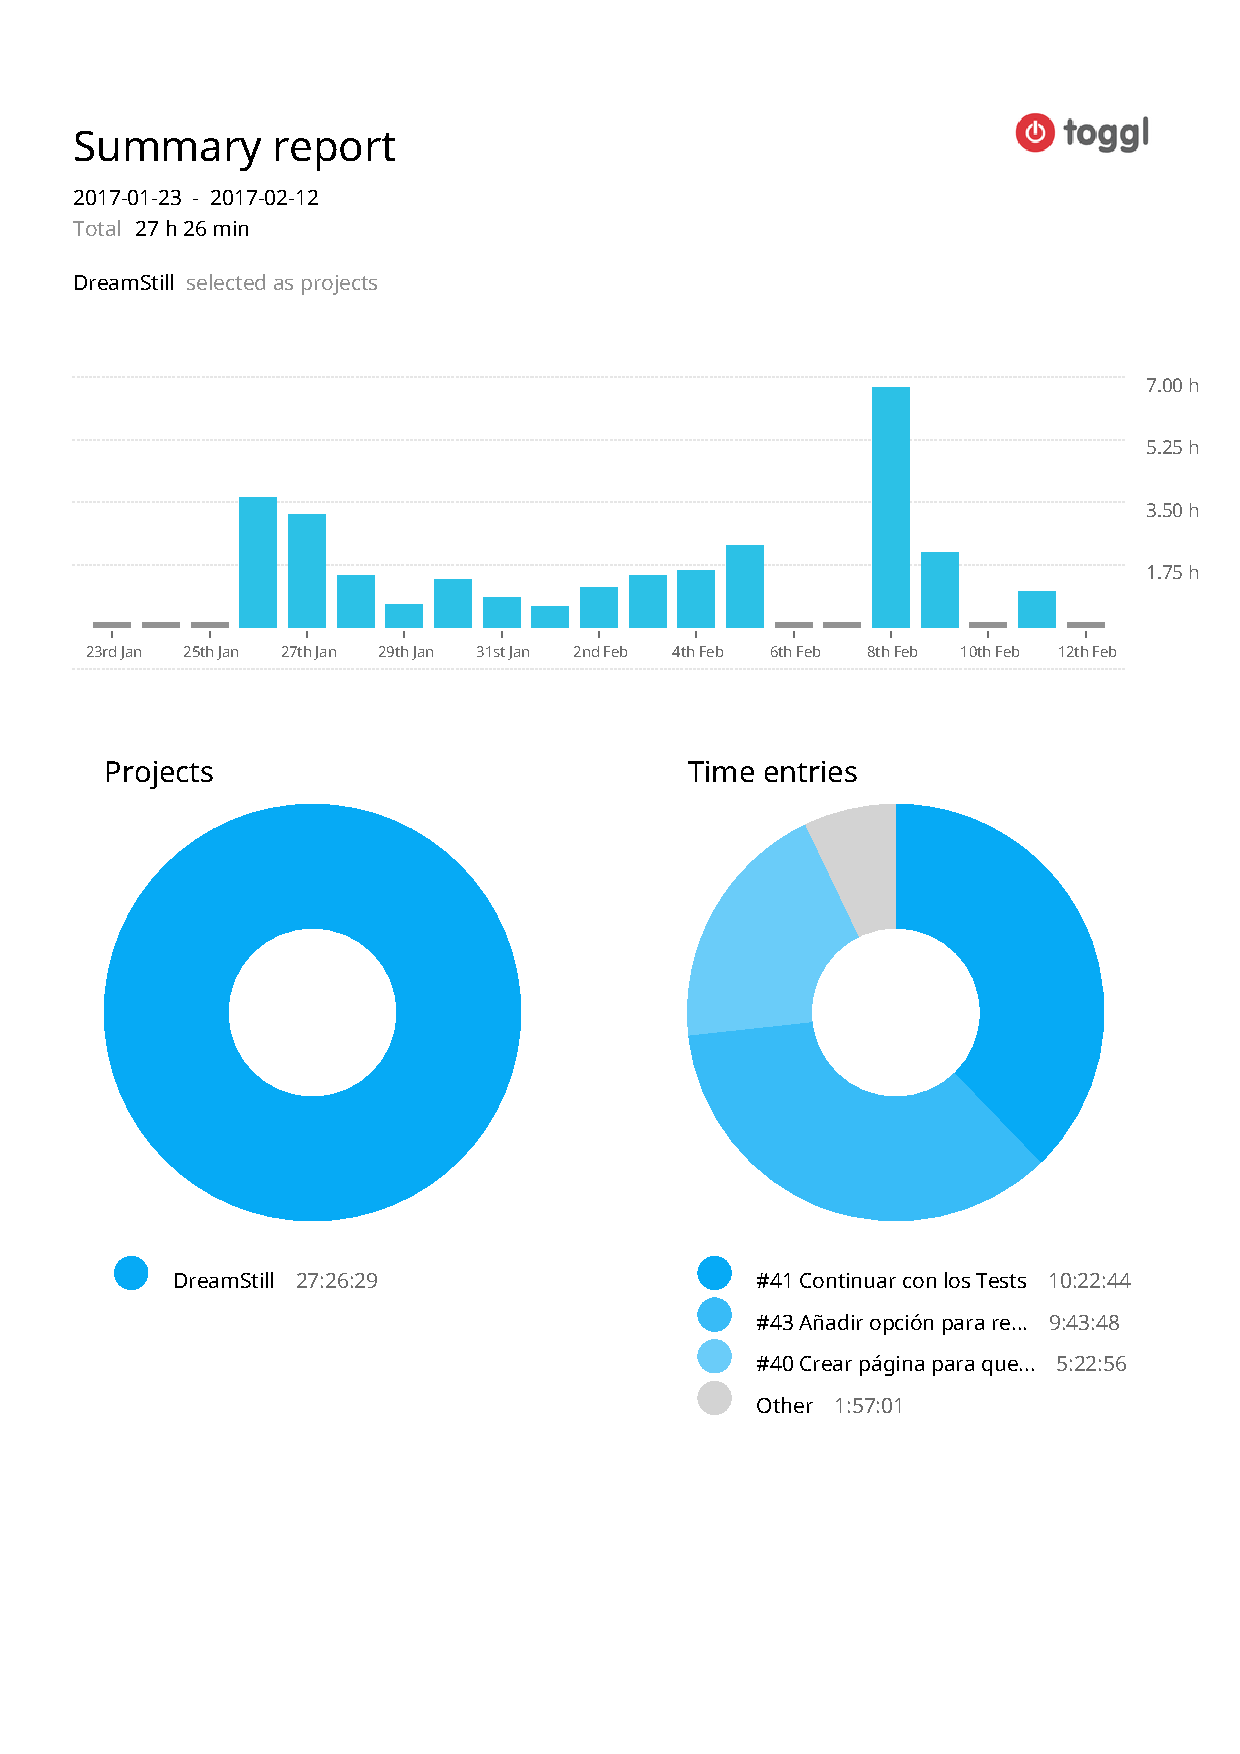
\includepdf[pages={1}]{togglReports/Sprint8.pdf}

\subsection{Sprint 9}

A lo largo del noveno Sprint, se comenzó con la documentación de la presente memoria. Concretamente, se introducieron los capítulos 1, 2 y 4.

- Burndown:

\begin{figure}[H]
\centering
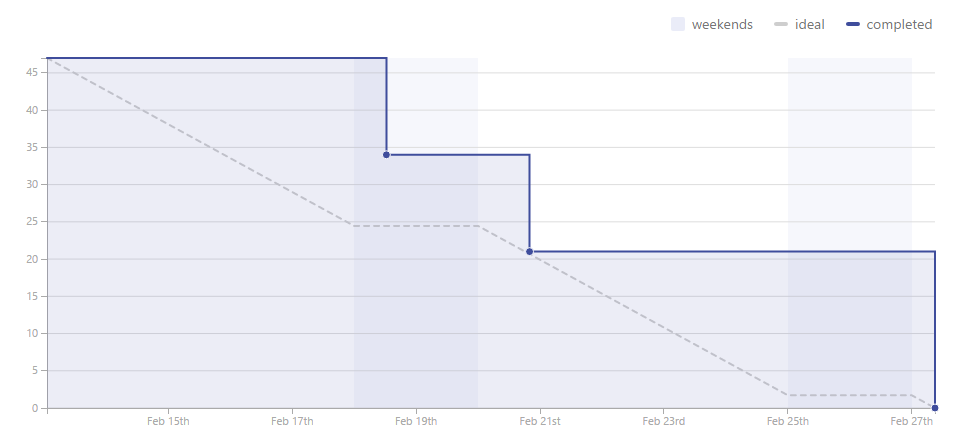
\includegraphics[totalheight=6cm]{burndowns/Sprint9.png}
\caption{Sprint 9}
\end{figure}

- Informe de Toggl:

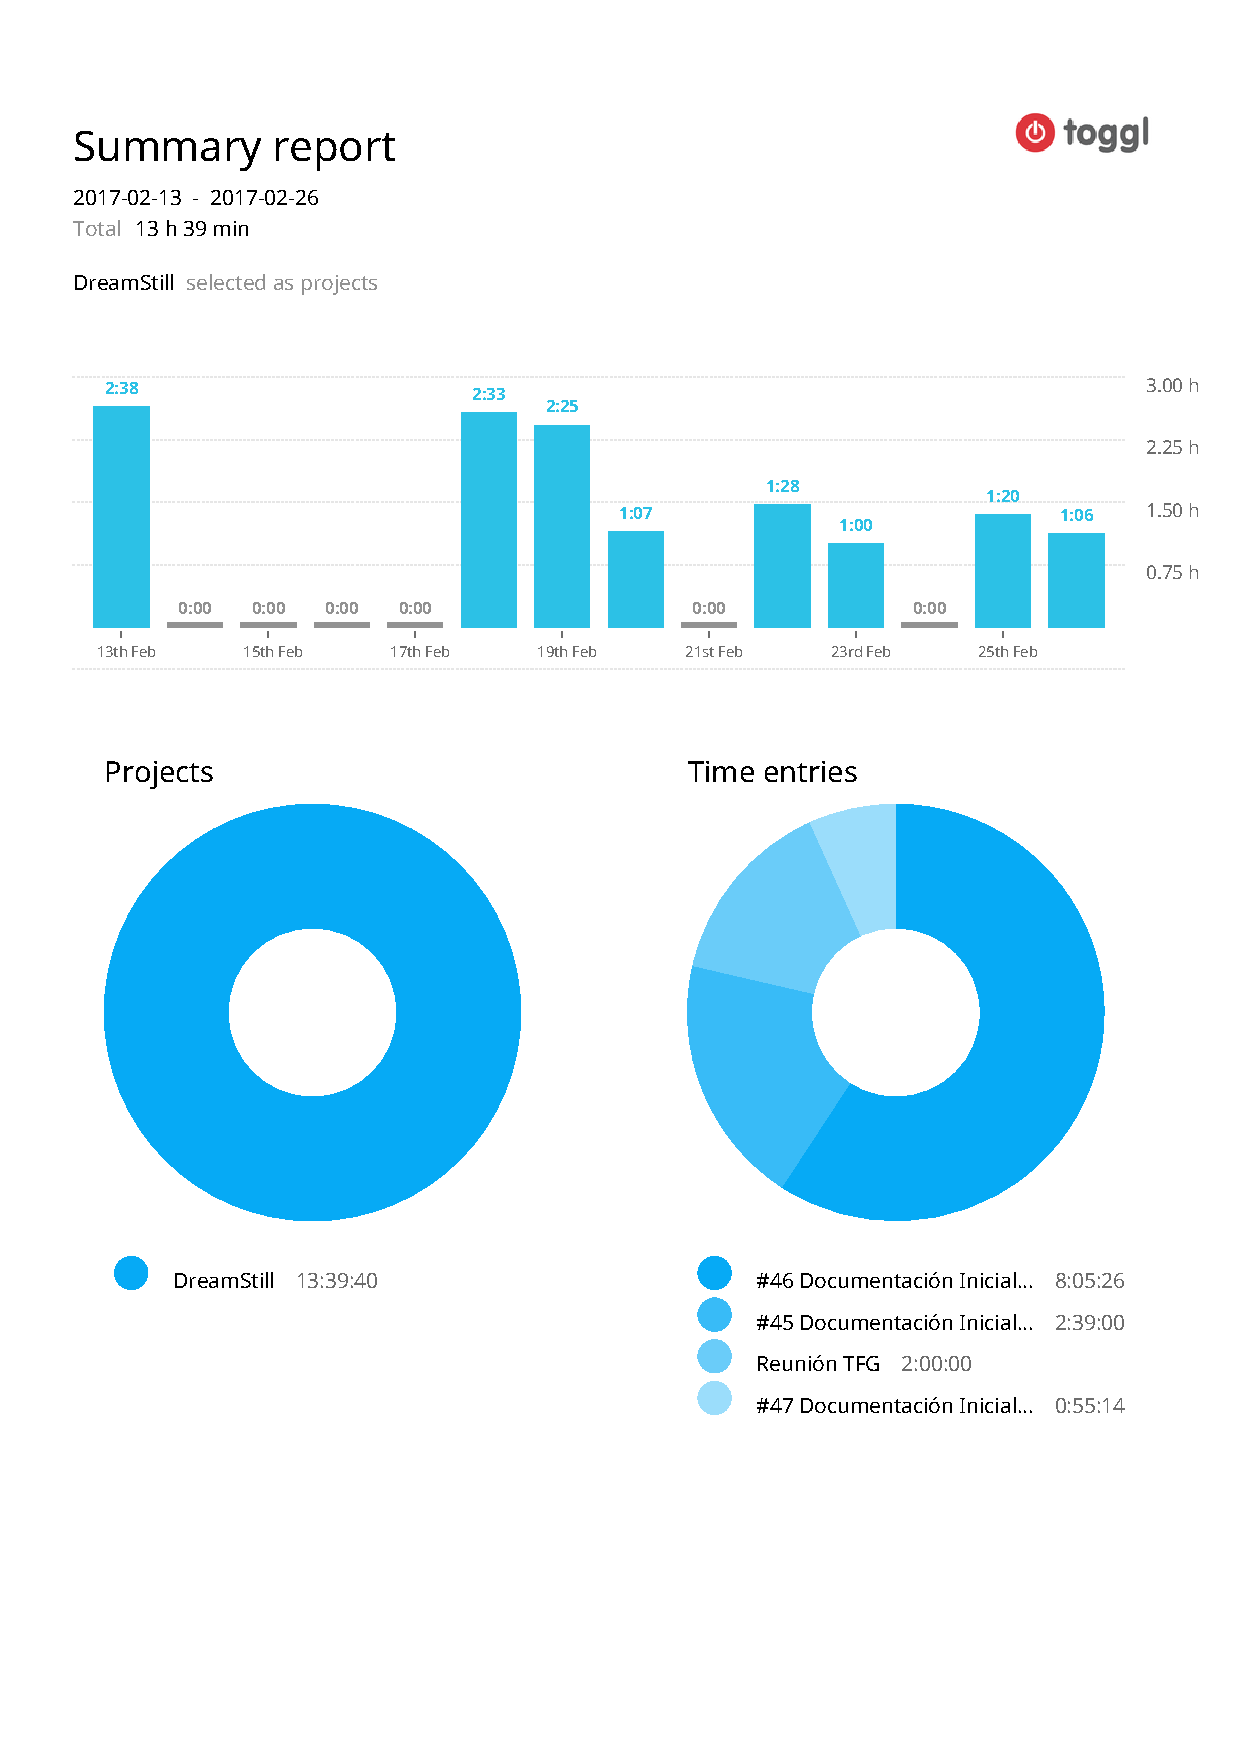
\includepdf[pages={1}]{togglReports/Sprint9.pdf}

\subsection{Sprint 10}

A lo largo del décimo Sprint, se revisaron los capítulos comenzados en el Sprint anterior y se añadió un sistema de alertas, para que el usuario pudiera activar unas alertas que le informaran de de carencias en su sueño durante un período determinado.

- Burndown:

\begin{figure}[H]
\centering
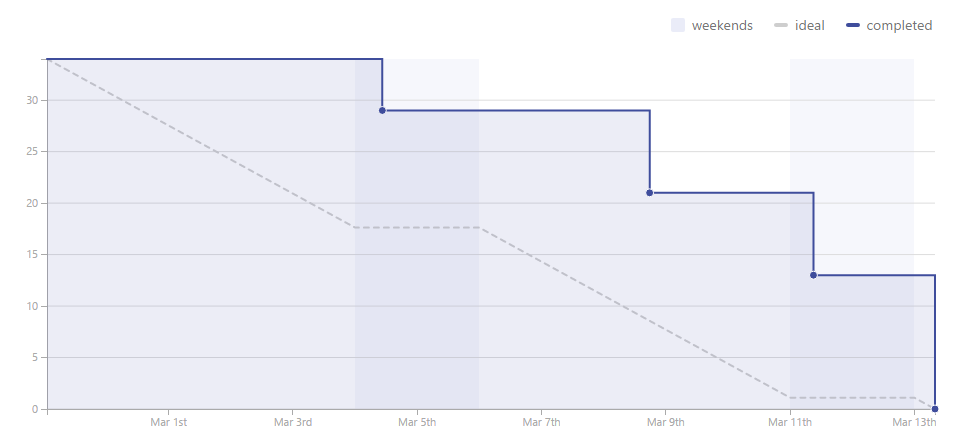
\includegraphics[totalheight=6cm]{burndowns/Sprint10.png}
\caption{Sprint 10}
\end{figure}

- Informe de Toggl:

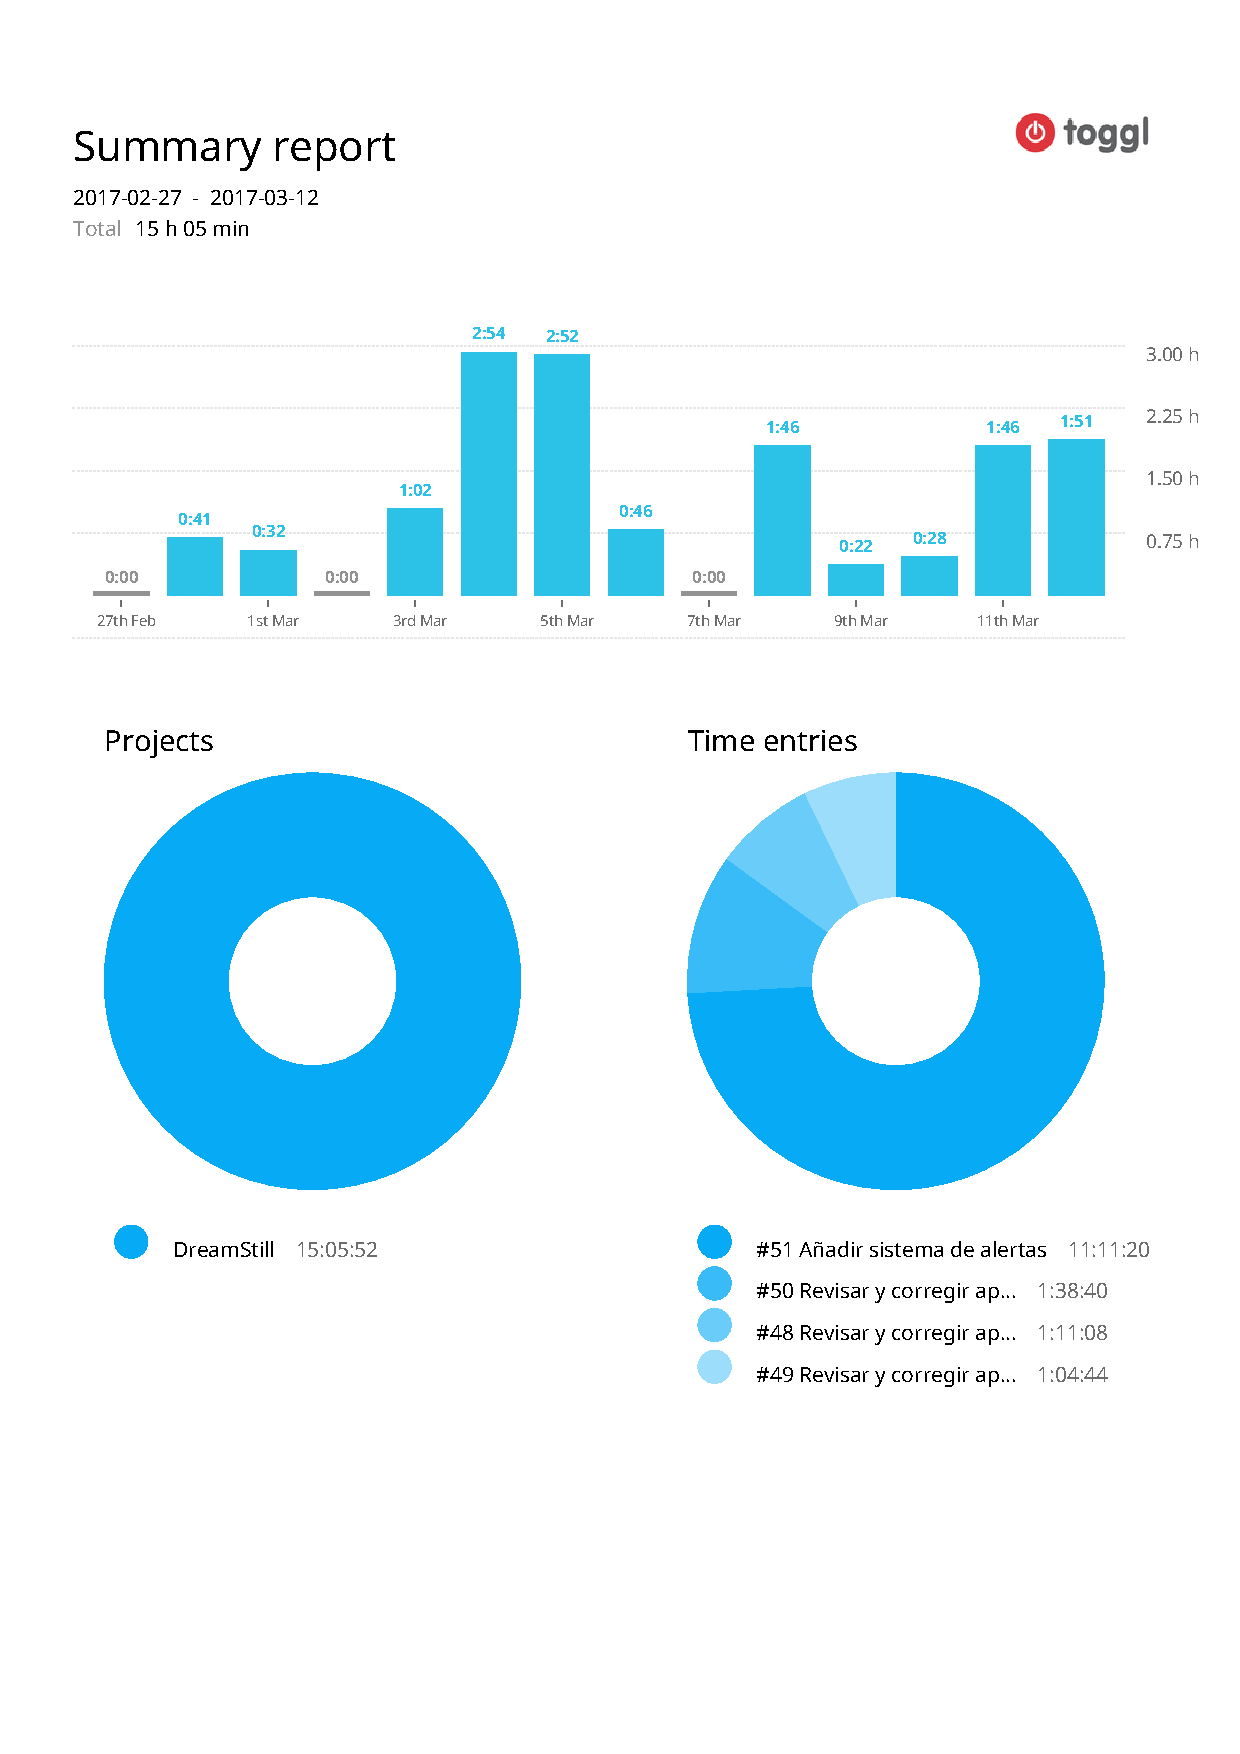
\includepdf[pages={1}]{togglReports/Sprint10.pdf}

\subsection{Sprint 11}

A lo largo del undécimo Sprint, se finalizó la documentación de los capítulos 1, 2 y 4 de la presente memoria y se introdujo la documentación de los apartados 1 y 7 de la presente memoria.

- Burndown:

\begin{figure}[H]
\centering
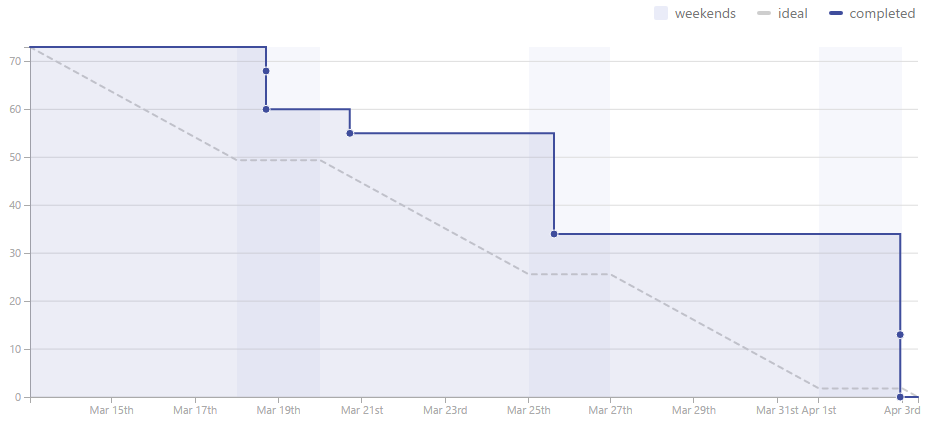
\includegraphics[totalheight=6cm]{burndowns/Sprint11.png}
\caption{Sprint 11}
\end{figure}

- Informe de Toggl:

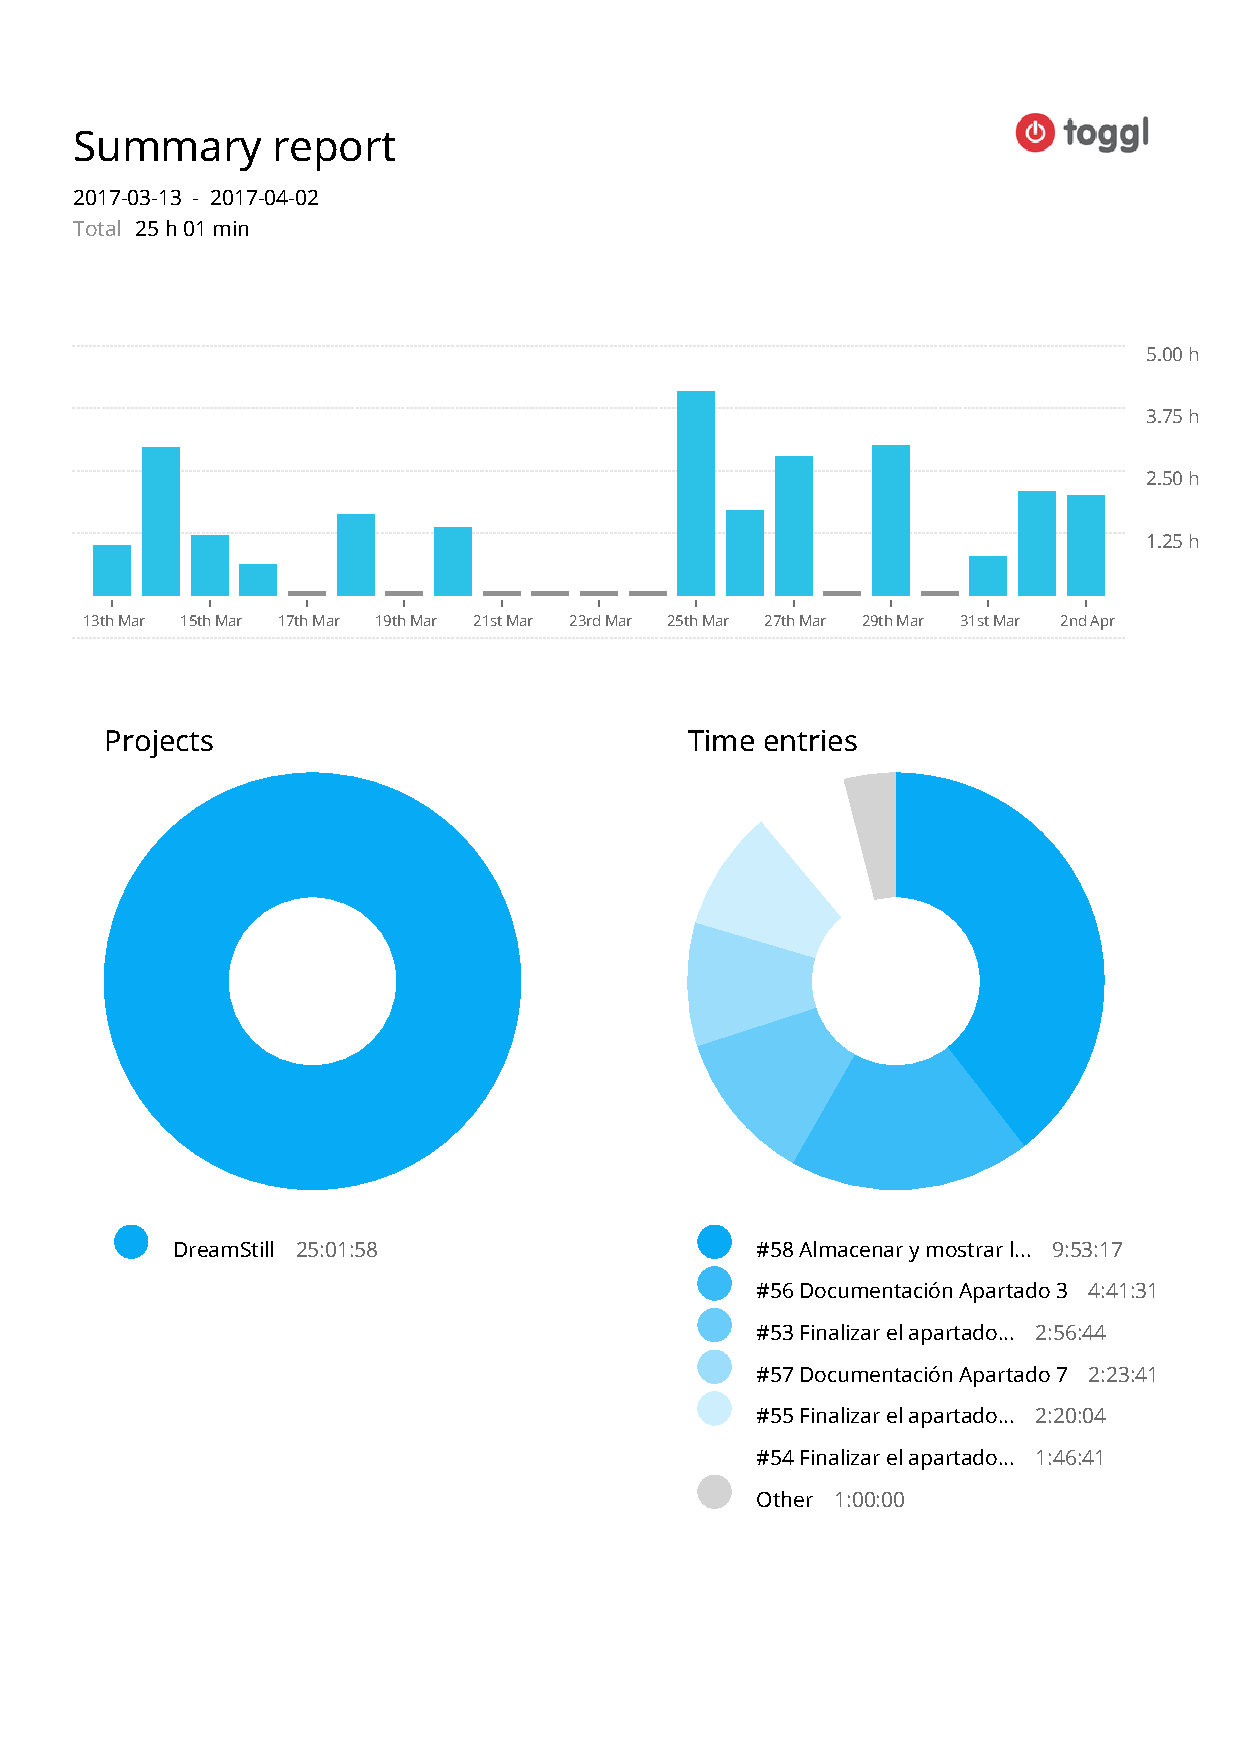
\includepdf[pages={1}]{togglReports/Sprint11.pdf}

\subsection{Sprint 12}

A lo largo del duodécimo Sprint, se finalizó la customización del sistema de alertas. Está customización consiste en ofrecer la posibilidad al usuario de elegir durante cuanto tiempo ha de incumplir un mínimo de horas durmiendo para que se le avise.

- Burndown:

\begin{figure}[H]
\centering
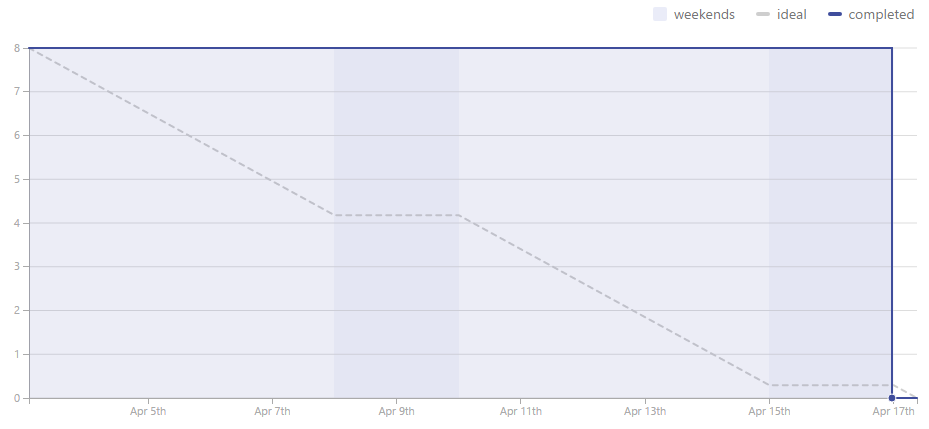
\includegraphics[totalheight=7cm]{burndowns/Sprint12.png}
\caption{Sprint 12}
\end{figure}

- Informe de Toggl:

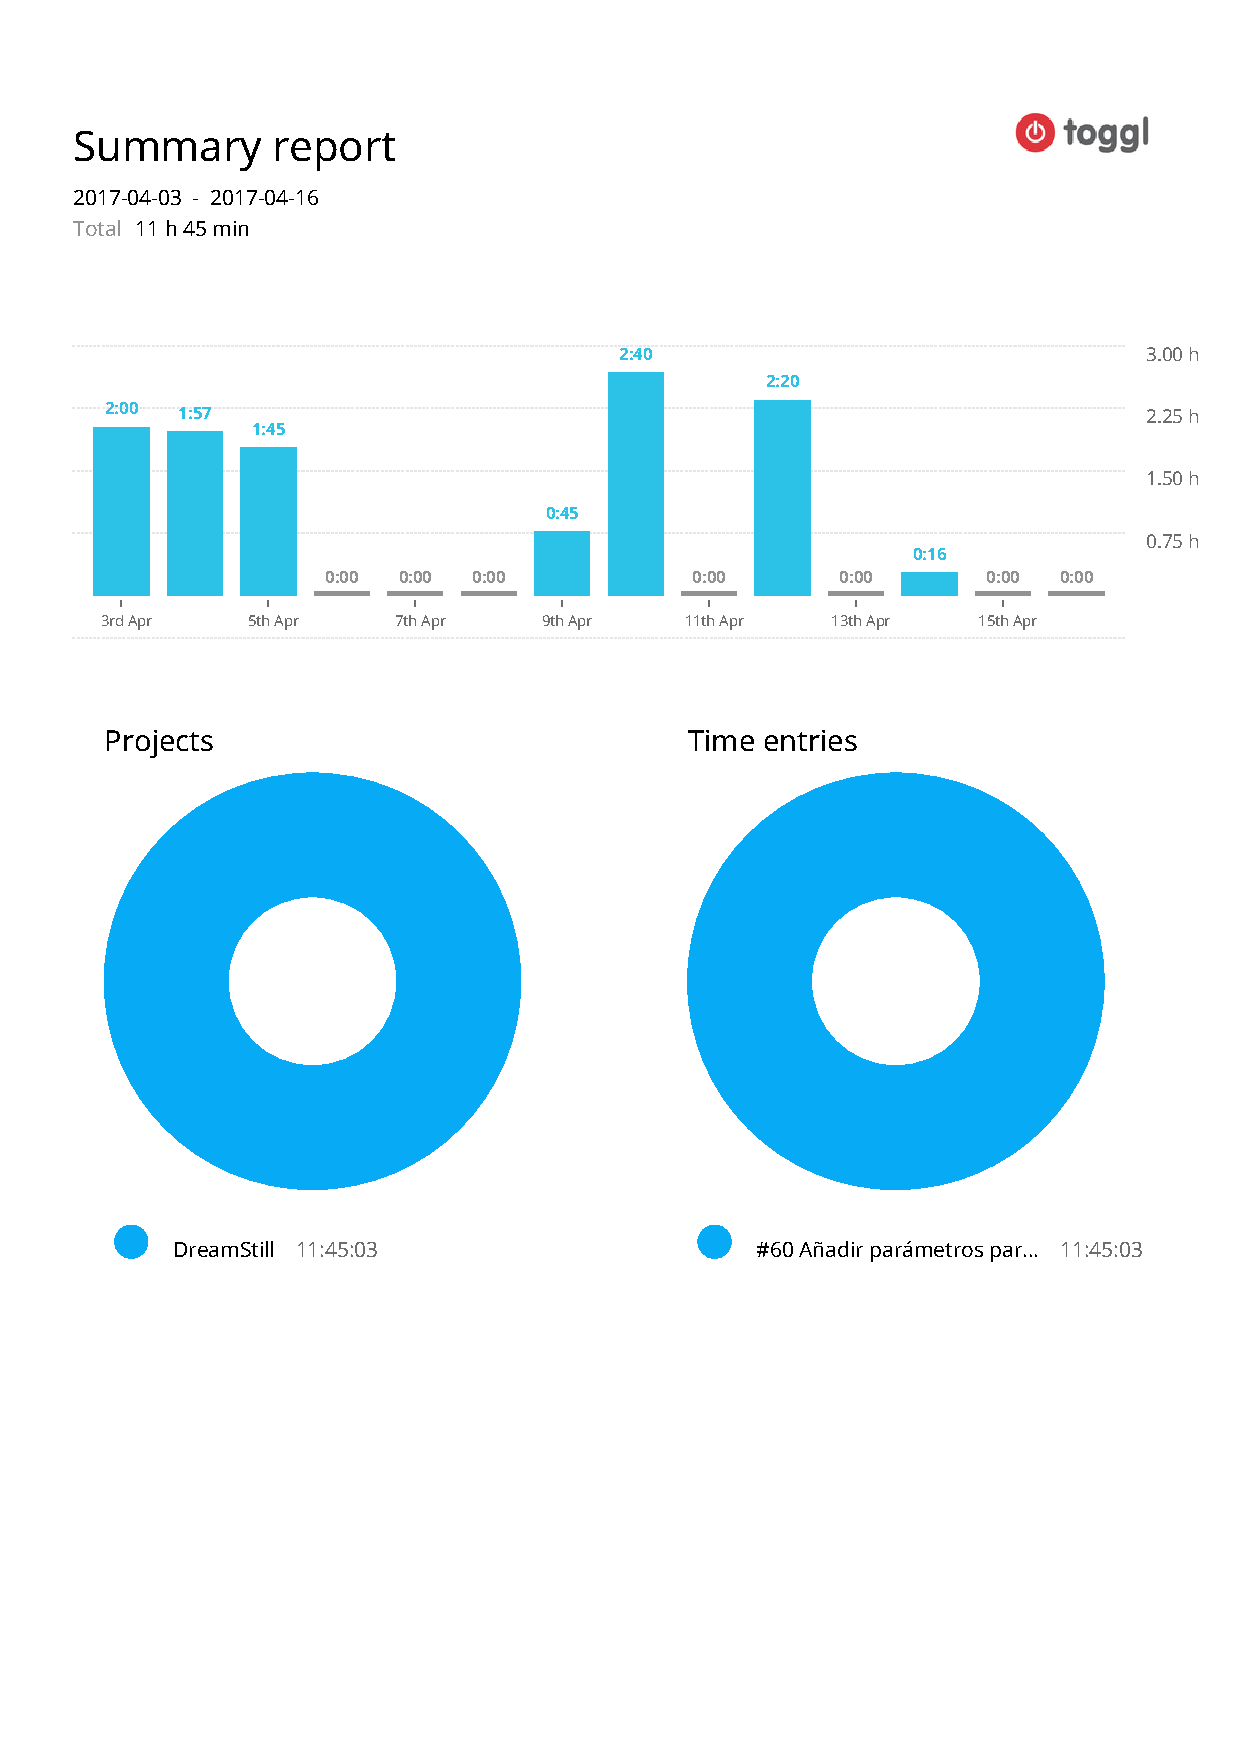
\includepdf[pages={1}]{togglReports/Sprint12.pdf}

\subsection{Sprint 13}

A lo largo del decimotercero Sprint, se finalizó con los apartados 6 y 8 de la documentación. Además, se corrigieron errores que se habían cometido en la documentación en las tareas anteriores.

- Burndown:

\begin{figure}[H]
\centering
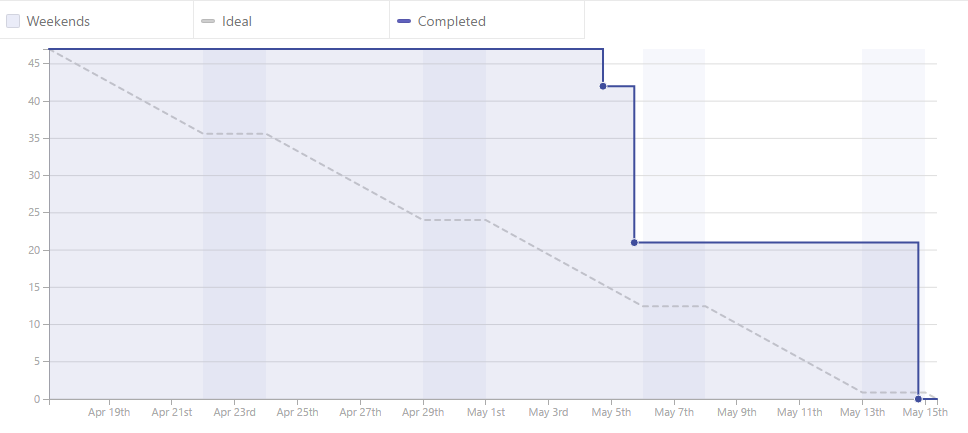
\includegraphics[totalheight=7cm]{burndowns/Sprint13.png}
\caption{Sprint 13}
\end{figure}

- Informe de Toggl:

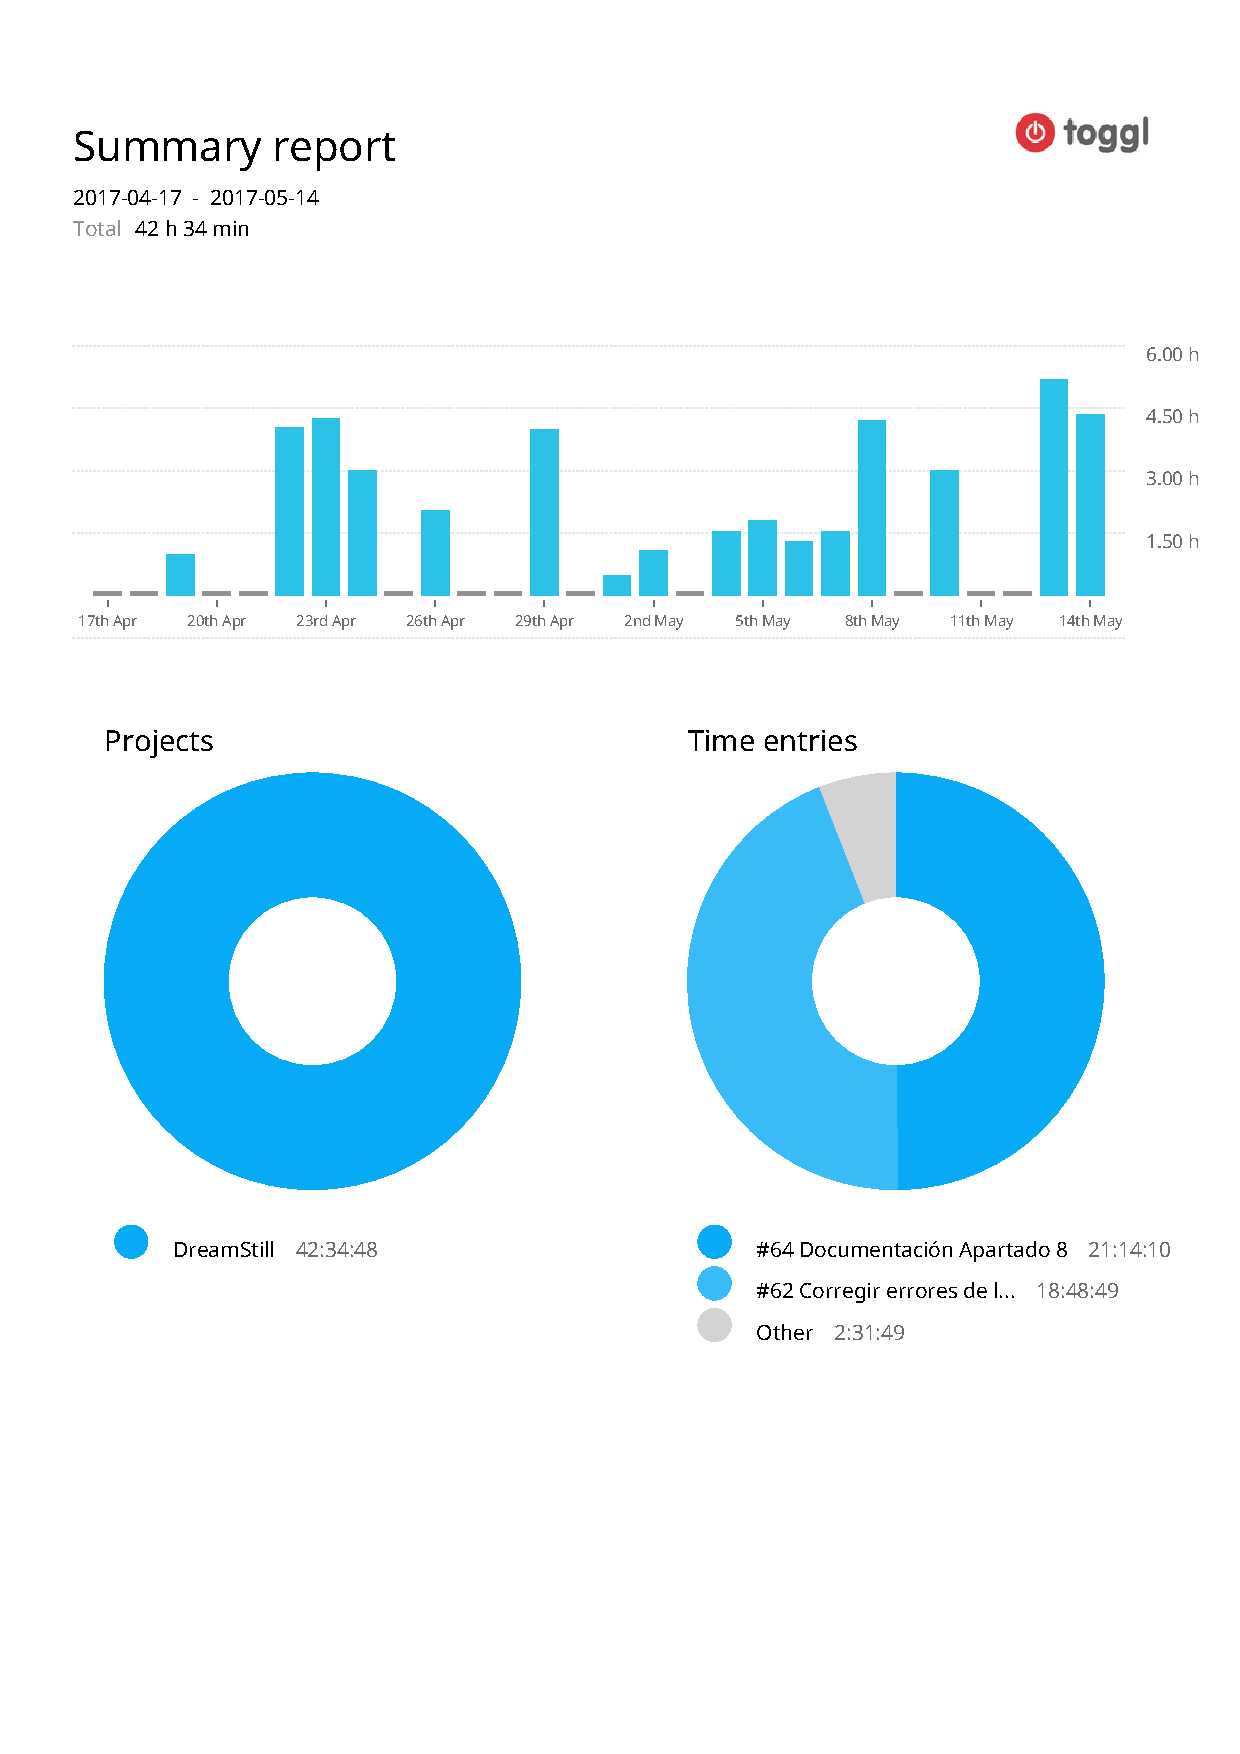
\includepdf[pages={1}]{togglReports/Sprint13.pdf}

\subsection{Sprint 14}

A lo largo del decimocuarto Sprint, se corrigieron los errores restantes en la documentación. Además, se realizó el presupuesto del presente TFG.

- Burndown:

\begin{figure}[H]
\centering
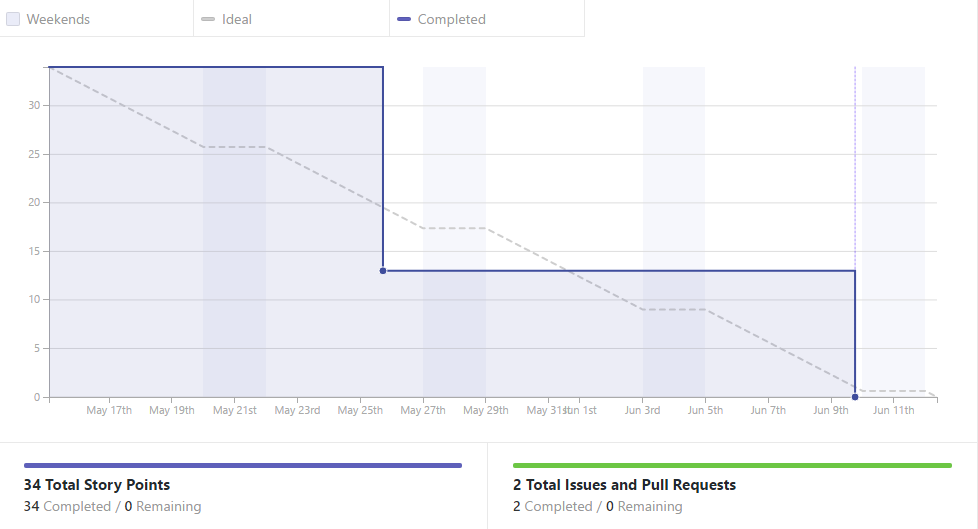
\includegraphics[totalheight=7cm]{burndowns/Sprint14.png}
\caption{Sprint 14}
\end{figure}

- Informe de Toggl:

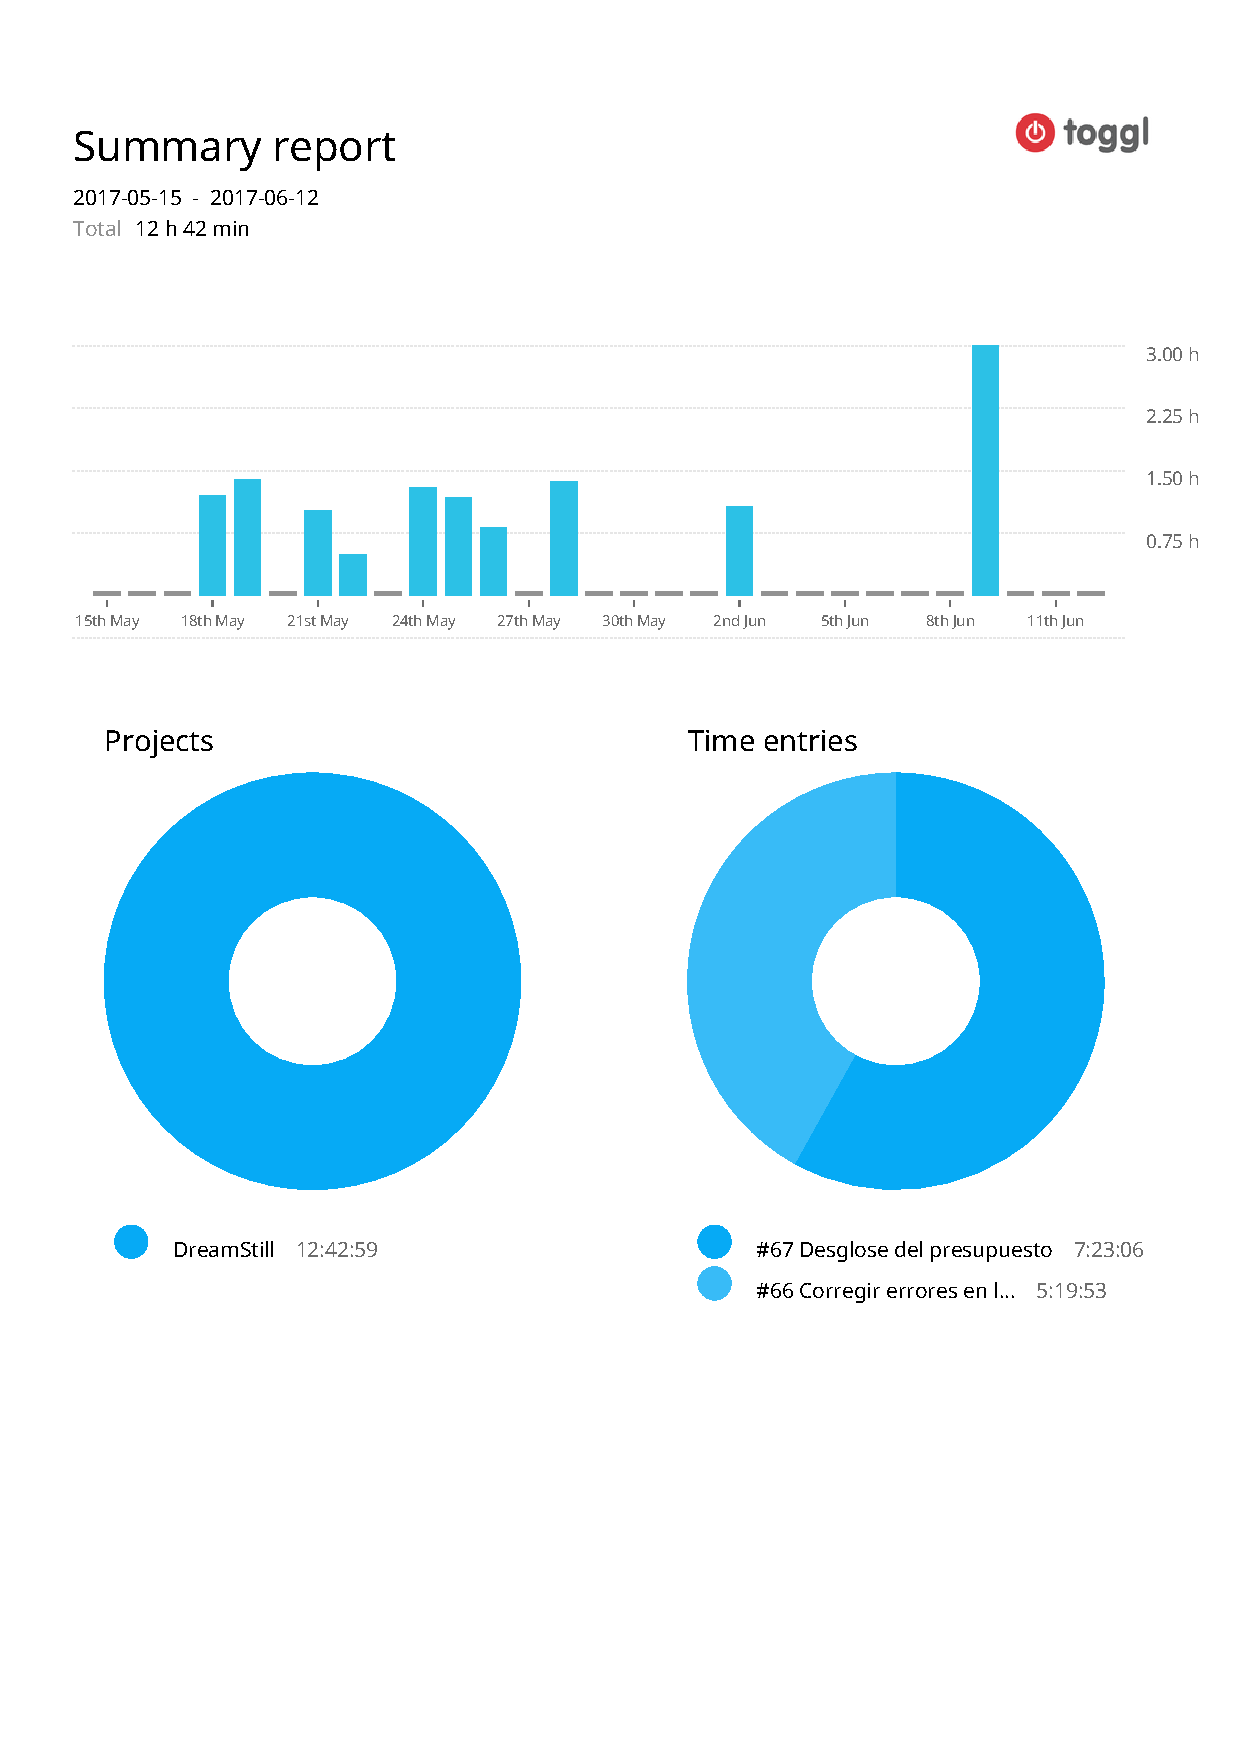
\includepdf[pages={1}]{togglReports/Sprint14.pdf}

\section{Presupuesto}

Para la elaboración del presupuesto, se han tenido en cuenta las distintas etapas y perfil que conforman la ejeución del TFG. 

Los sueldos establecidos han sido obtenidos a partir de datos oficiales de la Junta de Andalucía, con la finalidad de que sean lo más reales posibles y aproximar el presupuesto a un presupuesto que se mostraría en un desarrollo real. 

He de destacar la gran aportación que ha hecho Toggl en la elaboración del presupuesto, ya que gracias a tener registradas todas las tareas en el mismo, se ha podido obtener con gran exactitud el coste del mismo. Además, gracias a la claridad de los nombres de las tareas, se ha podido distinguir con bastante exactitud qué perfil ha realizado cada tarea.

La mayor parte del coste se invertirá en el pago de los sueldos a los distintos perfiles. Además de éste coste se han considerado otros aspectos los cuales creemos que han de estar en un presupuesto de un proyecto como éste.

Se han tenido en cuenta costes indirectos como (luz, agua o Internet) y además la amortización de los equipos necesarios para la realización de un proyecto. Para el cálculo de los costes indirectos se ha realizado un estudio del pago medio en una vivienda unifamiliar y se ha realizado una estimación de los costes a partir de la misma. Respecto a la amortización de equipos, sólo se ha utilizado un equipo, mi portátil personal valorado en 900 euros.

Además se han presupuestado los costes de Hosting (teniendo en cuenta los precios que nos ofrecen en DigitalOcean) y se ha calculado el alquiler derivado de dicho servicio. Respecto al mantenimiento, se ha presupuestado un mantenimiento de 6 meses. Este valor se ha obtenido de los plazos de mantenimiento que exige la Junta de Andalucía en muchos de sus proyectos Software. 

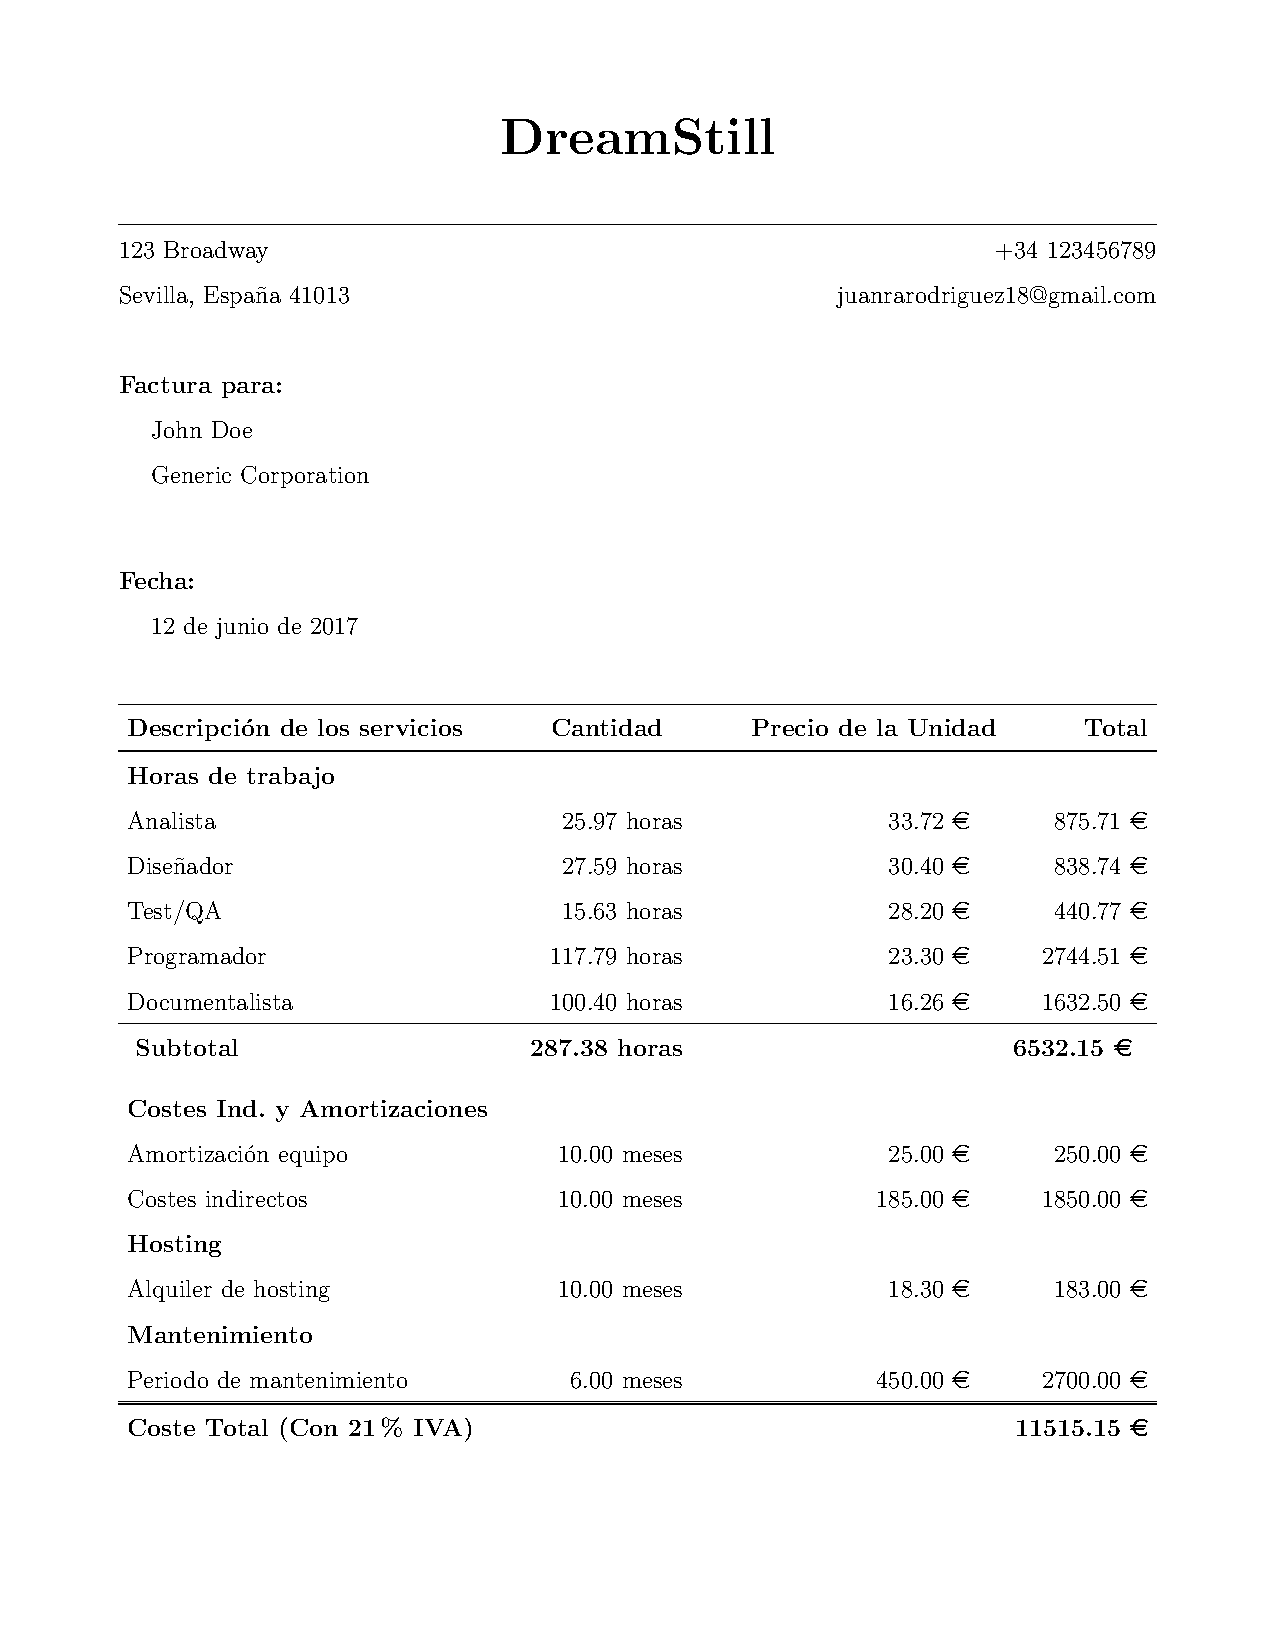
\includepdf[pages={1}]{invoice.pdf}

% 6. Pruebas y validación de la solución: (...)
\chapter{Pruebas y validación de la solución}

Teniendo presente las Historias de Usuario desarrolladas en el capítulo 6 se han realizado las pruebas de la aplicación. Gracias a las pruebas realizadas en la aplicación podremos comprobar que tanto las nuevas funcionalidades que se añadan en la aplicación como las ya existentes funcionan correctamente.

Se ha usado la herramienta Travis para la ejecución continua de las pruebas. Con cada ``commit'' (se considera commit la acción de subir nuevos cambios de código fuente a un sistema de control versiones) Travis ejecutará las pruebas de la aplicación y nos informará en el caso de que haya ocurrido un fallo en la ejecución de alguna de ellas.

Respecto a la validación de la solución, se considera válida aquella en la que las pruebas son exitosas y además se cumple con un mínimo de calidad, es decir, el resultado es similar al esperado y tiene un acabado aceptable. Siguiendo éste criterio se han validado las distintas funciones de la aplicación. 

A continuación se mostrará como se han realizados las pruebas para cada uno de las Historias de Usuario:

\pagebreak
\textbf{HU1 - Registro en la aplicación}:

\begin{itemize}
\item\textbf{Registrarse con los datos correctos y comprobar que efectivamente se realiza con éxito el registro}: Para ésta prueba se ha llevado a cabo una Validación Funcional manual. Se ha comprobado que un usuario puede introducir datos de registros y éstos se almacenan con éxito en la Base de Datos, completándose el registro en la aplicación con éxito.
\item\textbf{Revisar que al introducir datos erróneos la aplicación avisa de los fallos en esos datos}: Para ésta prueba se ha llevado a cabo una Validación Funcional manual. Se ha comprobado que al introducir datos erróneos en el formulario del registro o al dejar alguno de los campos del mismo en blanco, la aplicación impide el registro en la misma e informa de los errores cometidos.
\end{itemize}

{\tiny
\setlength{\LTleft}{-20cm plus -1fill}
\setlength{\LTright}{\LTleft}
\begin{center}
\begin{longtable}{| c | M{1.5cm} | M{1.5cm} | M{2.5cm} | M{1.5cm} | M{1.5cm} | M{1.5cm} | M{1.5cm} |}
\caption[Tabla de Pruebas - HU1]{Tabla de Pruebas - HU1} \label{grid_mlmmh} \\

\hline Automatizada & Prueba & Fecha & Datos de Entrada & Resultado & Esperado & Ejecutada por \\
\endfirsthead
\hline
No & Registrarse datos correctos & Enero 2017 & Nombre, email y contraseña de un nuevo usuario & El usuario se almacena en la aplicación & El usuario es almacenado en la aplicación & Juan Ramón Rodríguez \\
\hline
No & Revisar datos erróneos & Enero 2017 & Nombre, email y contraseña incorrectos de un nuevo usuario & La aplicación avisa de que los datos son incorrectos & La aplicación valida los datos correctamente & Juan Ramón Rodríguez \\
\hline
\end{longtable}
\end{center}}
 
\textbf{HU2 - Loguearse en la aplicación}:

\begin{itemize}
\item\textbf{Ingresar los datos de Login correctos y comprobar que se da acceso al usuario a la aplicación}: Para ésta prueba se ha llevado a cabo una Validación Funcional automatizada. El test automatizado comprueba que al introducir datos de ``login'' correctos se accede con éxito a la aplicación.
\item\textbf{Revisar que al introducir datos erróneos la aplicación avisa de que los datos introducidos no corresponden con los de ningún usuario registrado}: Para ésta prueba se ha llevado a cabo una Validación Funcional manual. Se ha comprobado que al introducir datos erróneos en el formulario de login o al dejar alguno de los campos del mismo en blanco la aplicación impide el acceso a la misma.
\end{itemize}
 
{\tiny
\setlength{\LTleft}{-20cm plus -1fill}
\setlength{\LTright}{\LTleft}
\begin{center}
\begin{longtable}{| c | M{1.5cm} | M{1.5cm} | M{2.5cm} | M{1.5cm} | M{1.5cm} | M{1.5cm} | M{1.5cm} |}
\caption[Tabla de Pruebas - HU2]{Tabla de Pruebas - HU2} \label{grid_mlmmh} \\

\hline Automatizada & Prueba & Fecha & Datos de Entrada & Resultado & Esperado & Ejecutada por \\
\endfirsthead
\hline
Si & Login datos correctos & Enero 2017 & Nombre y contraseña usuario & El usuario accede a la aplicación & El usuario obtiene acceso a la aplicación & Juan Ramón Rodríguez \\
\hline
No & Revisar datos erróneos & Enero 2017 & Nombre y contraseña incorrectos de un usuario & La aplicación avisa de que los datos son incorrectos & La aplicación valida los datos correctamente & Juan Ramón Rodríguez \\
\hline
\end{longtable}
\end{center}}

\textbf{HU3 - Acceder a la página principal}:
 
\begin{itemize}
\item\textbf{Comprobar que los datos que se le muestran al usuario son los pertenecientes a ese usuario}: Para ésta prueba se ha llevado a cabo una Validación Funcional automatizada. El test automatizado comprueba que cuando un usuario accede a la Página Principal se le muestran los eventos registrados en la Base de Datos de sus datos de sueño.
\item\textbf{Revisar que todos los enlaces funcionan correctamente y que no hay ningún error a la hora de extraer los datos de la base de datos}: Para ésta prueba se ha llevado a cabo una Validación Funcional automatizada. El test automatizado comprueba que los enlaces en la Página Principal funcionan correctamente.
\end{itemize}

{\tiny
\setlength{\LTleft}{-20cm plus -1fill}
\setlength{\LTright}{\LTleft}
\begin{center}
\begin{longtable}{| c | M{1.5cm} | M{1.5cm} | M{2.5cm} | M{1.5cm} | M{1.5cm} | M{1.5cm} | M{1.5cm} |}
\caption[Tabla de Pruebas - HU3]{Tabla de Pruebas - HU3} \label{grid_mlmmh} \\

\hline Automatizada & Prueba & Fecha & Datos de Entrada & Resultado & Esperado & Ejecutada por \\
\endfirsthead
\hline
Si & Datos mostrados correctos & Enero 2017 & Nombre y contraseña de un usuario & El usuario accede a sus datos correctamente & El usuario obtiene acceso a sus datos & Juan Ramón Rodríguez \\
\hline
Si & Enlaces correctos & Enero 2017 & Nombre y contraseña de un usuario & Todos los enlaces funcionan correctamente & Los enlaces funcionan correctamente & Juan Ramón Rodríguez \\
\hline
\end{longtable}
\end{center}}
 
\pagebreak
\textbf{HU4 - Gestión de datos de perfil y validación}:
 
\begin{itemize}
\item\textbf{Comprobar que los datos introducidos se procesan con éxito}: Para ésta prueba se ha llevado a cabo una Validación Funcional manual. Se ha comprobado que al introducir datos tanto en el formulario de registro como de login de la aplicación estos se guardan exactamente como se han introducido en la aplicación.
\item\textbf{Revisar la validación de datos al introducir datos erróneos}: Para ésta prueba se ha llevado a cabo una Validación Funcional manual. Se ha comprobado que al introducir datos erroneos tanto en el formulario de registro como de login, la aplicación informa de que estos datos son erróneos.
\end{itemize}

{\tiny
\setlength{\LTleft}{-20cm plus -1fill}
\setlength{\LTright}{\LTleft}
\begin{center}
\begin{longtable}{| c | M{1.5cm} | M{1.5cm} | M{2.5cm} | M{1.5cm} | M{1.5cm} | M{1.5cm} | M{1.5cm} |}
\caption[Tabla de Pruebas - HU4]{Tabla de Pruebas - HU4} \label{grid_mlmmh} \\

\hline Automatizada & Prueba & Fecha & Datos de Entrada & Resultado & Esperado & Ejecutada por \\
\endfirsthead
\hline
No & Datos procesados correctos & Enero 2017 & Datos de un usuario & Los datos se almacenan correctamente & Los datos son almacenados correctamente & Juan Ramón Rodríguez \\
\hline
No & Validación de datos & Enero 2017 & Datos incorrectos de un usuario & La aplicación informa de los errores & La validación funciona con éxito & Juan Ramón Rodríguez \\
\hline
\end{longtable}
\end{center}}
 
\textbf{HU5 - Representación de datos de Firebase en el calendario}:
 
\begin{itemize}
\item\textbf{Comprobar que los días que contienen datos de sueño se marcan en el calendario como un evento}: Para ésta prueba se ha llevado a cabo una Validación Funcional automatizada. El test automatizado comprueba que en un mes determinado se le muestran en el calendario los mismos eventos que hay almacenados en Firebase.
\end{itemize}

{\tiny
\setlength{\LTleft}{-20cm plus -1fill}
\setlength{\LTright}{\LTleft}
\begin{center}
\begin{longtable}{| c | M{1.5cm} | M{1.5cm} | M{2.5cm} | M{1.5cm} | M{1.5cm} | M{1.5cm} | M{1.5cm} |}
\caption[Tabla de Pruebas - HU5]{Tabla de Pruebas - HU5} \label{grid_mlmmh} \\

\hline Automatizada & Prueba & Fecha & Datos de Entrada & Resultado & Esperado & Ejecutada por \\
\endfirsthead
\hline
Si & Eventos representado con éxito & Febrero 2017 & Datos y eventos de un usuario & Los eventos se muestran en el calendario & Los eventos son mostrados en el calendario & Juan Ramón Rodríguez \\
\hline
\end{longtable}
\end{center}}
 
\textbf{HU6 - Integración de identificación en servicios de 3ºs en los datos de perfil}:
 
\begin{itemize}
\item\textbf{Comprobar que la integración con éstos servicios se hace correctamente}: Para ésta prueba se ha llevado a cabo una Validación Funcional manual. Se ha comprobado que la aplicación obtiene con éxito los datos de las distintas fuentes configuradas en el perfil de un usuario.
\item\textbf{Verificar la correcta identificación en dichos servicios}: Para ésta prueba se ha llevado a cabo una Validación Funcional manual. Se ha comprobado que la aplicación se identifica con éxito con los servicios configurados en el perfil de un usuario.
\end{itemize}

{\tiny
\setlength{\LTleft}{-20cm plus -1fill}
\setlength{\LTright}{\LTleft}
\begin{center}
\begin{longtable}{| c | M{1.5cm} | M{1.5cm} | M{2.5cm} | M{1.5cm} | M{1.5cm} | M{1.5cm} | M{1.5cm} |}
\caption[Tabla de Pruebas - HU6]{Tabla de Pruebas - HU6} \label{grid_mlmmh} \\

\hline Automatizada & Prueba & Fecha & Datos de Entrada & Resultado & Esperado & Ejecutada por \\
\endfirsthead
\hline
No & Comprobar Integración Servicios 3ºs & Febrero 2017 & Datos de un usuario & La integración se realiza correctamente & La integraicón se realiza con éxito & Juan Ramón Rodríguez \\
\hline
No & Correcta identificación en Servicios & Febrero 2017 & Datos de un usuario & La aplicación reconoce la identificación del usuario en el Servicio & La aplicación reconoce la correcta identificación del usuario en el Servicio & Juan Ramón Rodríguez \\
\hline
\end{longtable}
\end{center}}
 
\textbf{HU7 -  Acceder a la página de ``Resumen de Sueño'' para un día concreto}:

\begin{itemize}
\item\textbf{Comprobar que los datos que se le muestran al usuario son los pertenecientes a ese usuario}: Para ésta prueba se ha llevado a cabo una Validación Funcional manual. Se ha comprobado que la aplicación muestra sólo los datos de sueño del usuario que accede a la aplicación.
\item\textbf{Revisar que no hay ningún error a la hora de extraer los datos de la base de datos}: Para ésta prueba se ha llevado a cabo una Validación Funcional manual. Se ha comprobado que la aplicación muestra en las gráficas de ``Resumen de Sueño'' de un usuario los datos almacenados en la Base de Datos, sin que exista ningún error en ellos.
\end{itemize}

{\tiny
\setlength{\LTleft}{-20cm plus -1fill}
\setlength{\LTright}{\LTleft}
\begin{center}
\begin{longtable}{| c | M{1.5cm} | M{1.5cm} | M{2.5cm} | M{1.5cm} | M{1.5cm} | M{1.5cm} | M{1.5cm} |}
\caption[Tabla de Pruebas - HU7]{Tabla de Pruebas - HU7} \label{grid_mlmmh} \\

\hline Automatizada & Prueba & Fecha & Datos de Entrada & Resultado & Esperado & Ejecutada por \\
\endfirsthead
\hline
No & Comprobar datos Usuario ``Resumen de Sueño'' & Febrero 2017 & Datos de un usuario y eventos de sueño & Se muestran sólo los datos de ese usuario & Los datos de sólo ese usuario se muestran correctamente & Juan Ramón Rodríguez \\
\hline
No & Correcta extracción de los datos de la BD & Febrero 2017 & Datos de un usuario y eventos de sueño & No existen errores en los datos mostrados & Los datos mostrados no continen ningún error & Juan Ramón Rodríguez \\
\hline
\end{longtable}
\end{center}}
 
\textbf{HU8 - Terminar el proceso ``batch'' para que procese todos los mails de un usuario}:

\begin{itemize}
\item\textbf{Comprobar que se procesan los email pendientes correctamente}: Para ésta prueba se ha llevado a cabo una Validación Funcional manual. Se ha comprobado que todos los emails pendientes de la aplicación se procesan y almacenan con éxito.
\item\textbf{Verificar que el proceso se ejecuta cada vez que se inicia la aplicación}: Para ésta prueba se ha llevado a cabo una Validación Funcional manual. Se ha comprobado que cada vez que la aplicación se inicia, se inicia el proceso para la lectura de los mails de la aplicación.
\end{itemize}

{\tiny
\setlength{\LTleft}{-20cm plus -1fill}
\setlength{\LTright}{\LTleft}
\begin{center}
\begin{longtable}{| c | M{1.5cm} | M{1.5cm} | M{2.5cm} | M{1.5cm} | M{1.5cm} | M{1.5cm} | M{1.5cm} |}
\caption[Tabla de Pruebas - HU8]{Tabla de Pruebas - HU8} \label{grid_mlmmh} \\

\hline Automatizada & Prueba & Fecha & Datos de Entrada & Resultado & Esperado & Ejecutada por \\
\endfirsthead
\hline
No & Comprobar procesado de emails & Marzo 2017 & Emails de usuarios & Los emails pendientes se procesan correctamente & Los emails pendientes se procesan con éxito & Juan Ramón Rodríguez \\
\hline
No & Verificar la ejecución del proceso al inicio & Marzo 2017 & Emails de usuarios & El proceso se inicia y reconoce los emails correctamente & El proceso se inicia y reconoce los emails con éxito & Juan Ramón Rodríguez \\
\hline
\end{longtable}
\end{center}}

% 7.Manual de usuario
\chapter{Manual de usuario}

Basándonos en las Historias de Usuario definidas para el proyecto, se va a desarrollar el presente capítulo. En éste, se pretende que el lector entienda el funcionamiento de la aplicación y el flujo a seguir en ésta para realizar las distintas actividades que la misma ofrece. Para ello, se dividirá el capítulo en distintos apartados, con el objetivo de explicar en cada uno de ellos una funcionalidad relevante de la aplicación.

\pagebreak
\section{Registro en la aplicación}

Para proceder al registro en la aplicación, accederemos a la Página de Inicio de ésta.

\begin{figure}[H]
\centering
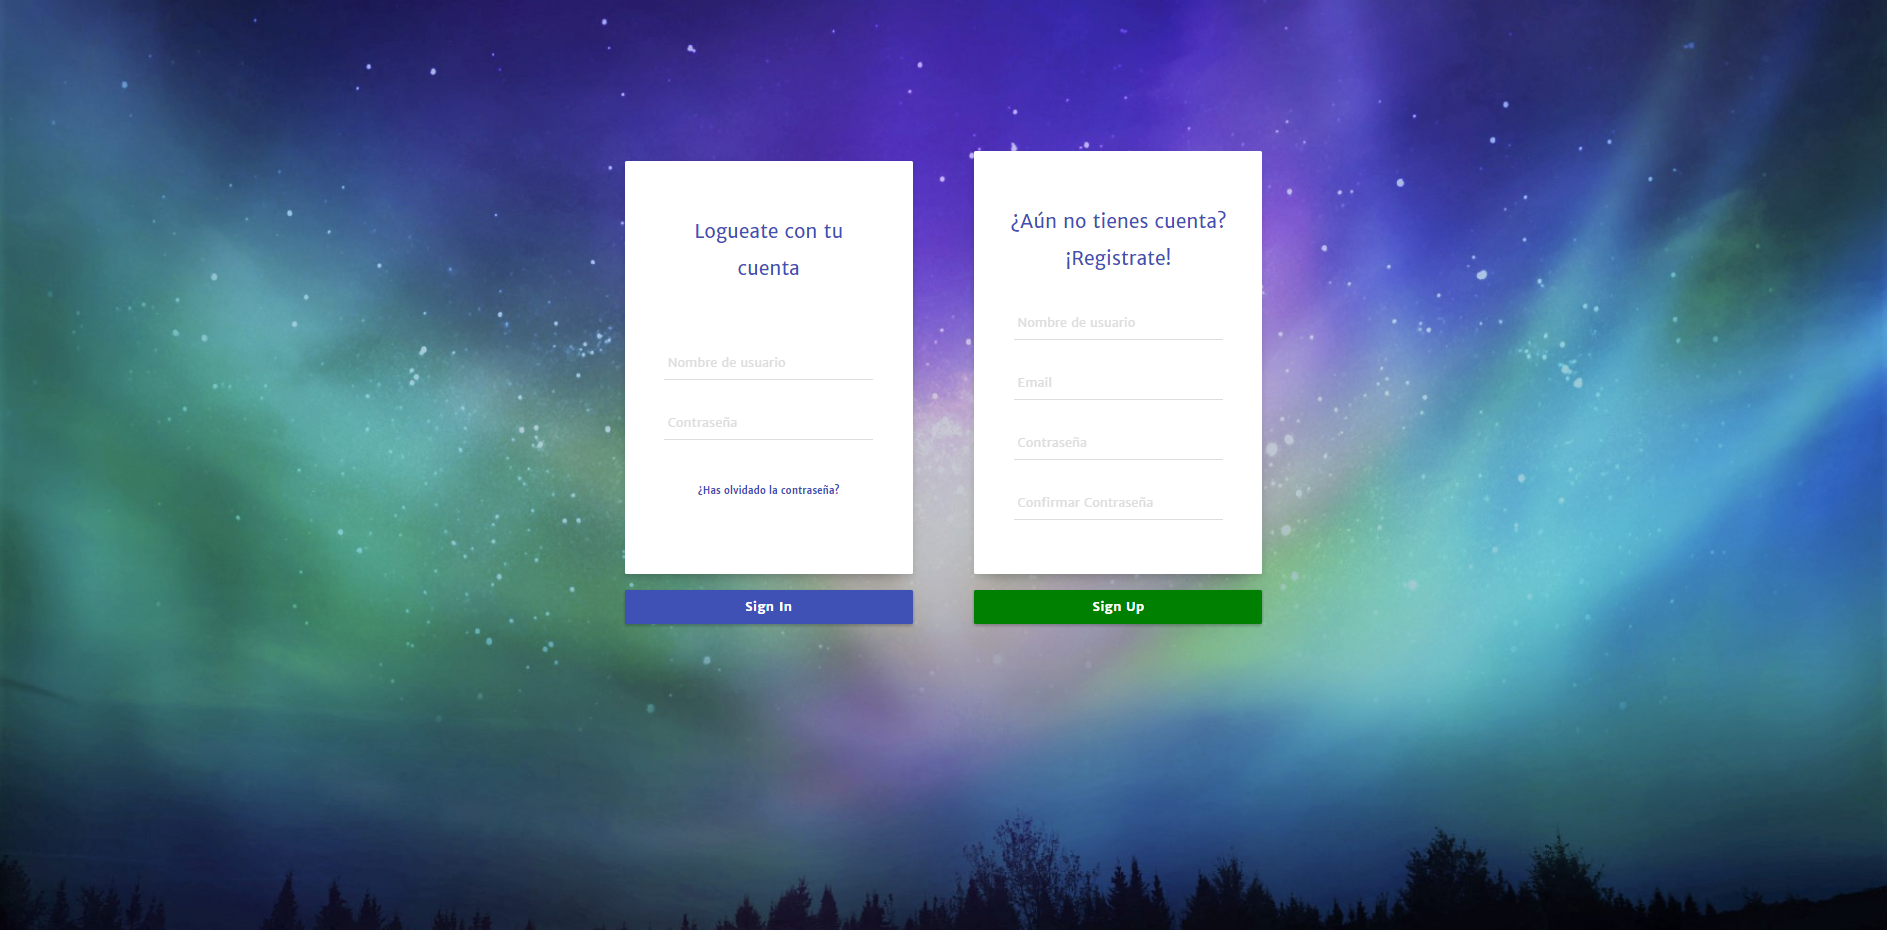
\includegraphics[totalheight=6cm]{manualUsuario/paginaInicio.png}
\caption{Página de Inicio}
\end{figure}

\pagebreak
Una vez nos encontremos en la Página de Inicio, nos encontraremos con dos formularios. Para proceder al registro deberemos de rellenar correctamente los datos del formulario de la derecha y pulsar sobre el botón de ``Sign Up''. 

\begin{figure}[H]
\centering
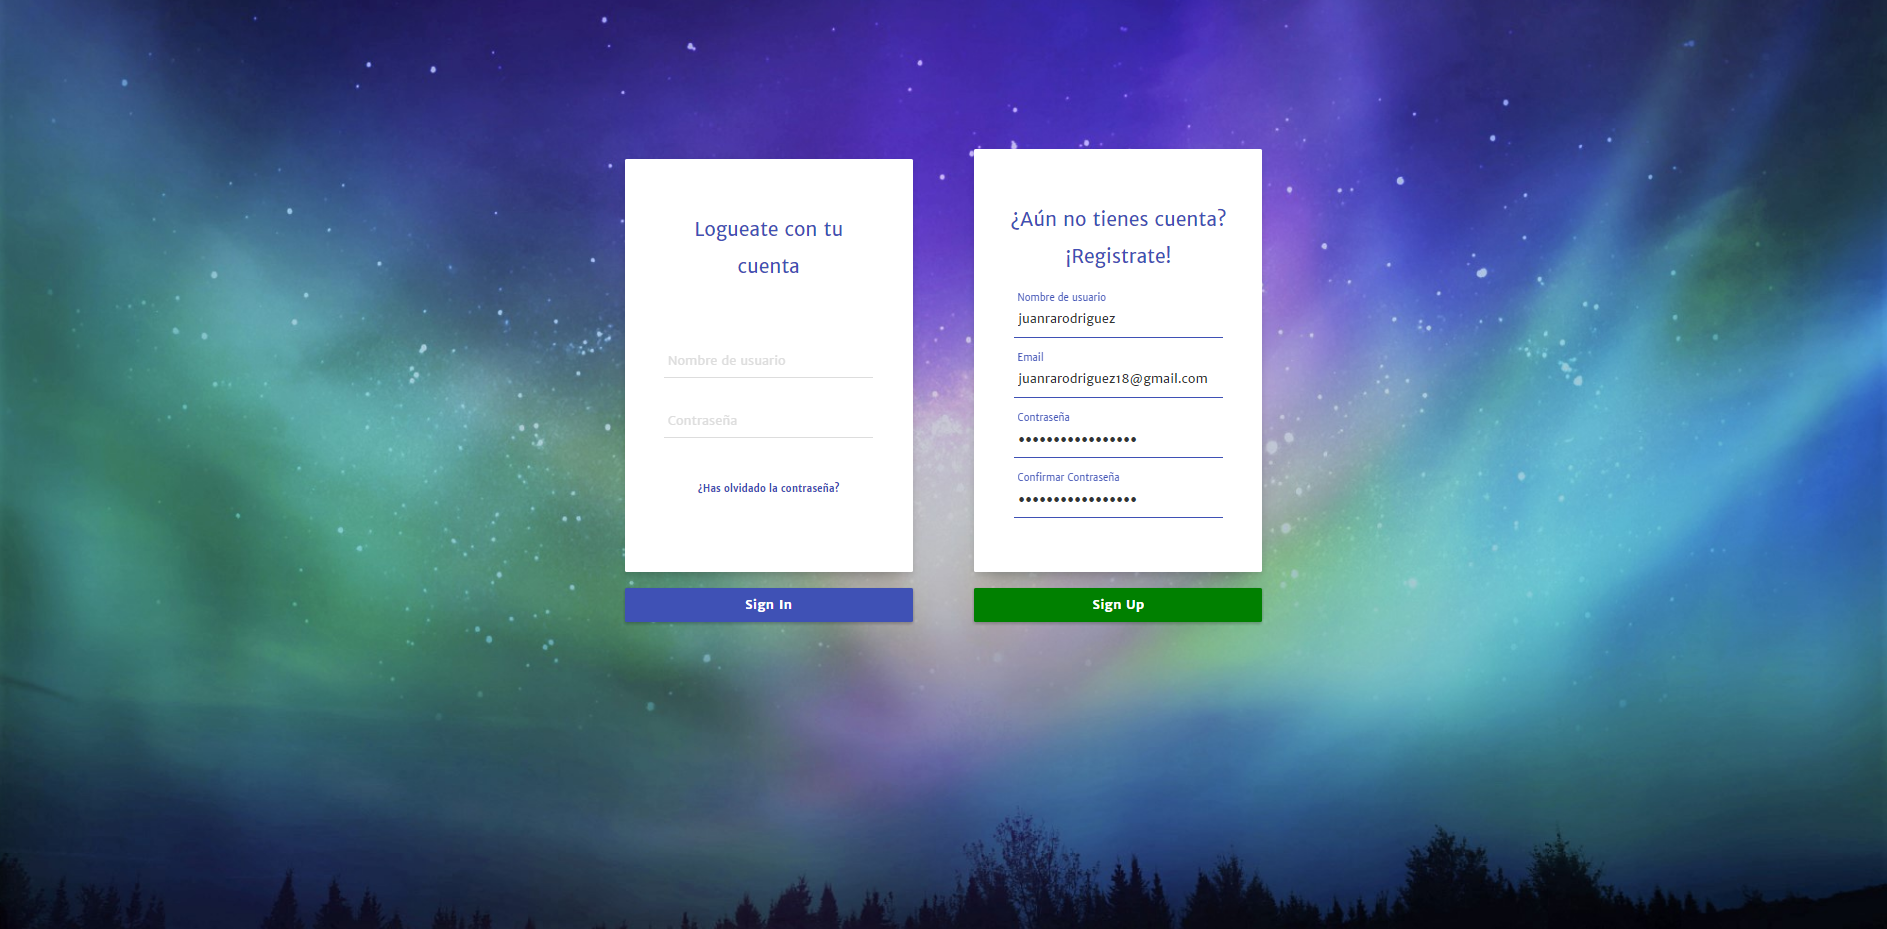
\includegraphics[totalheight=6cm]{manualUsuario/registro.png}
\caption{Página de Inicio - Registro}
\end{figure}

Si se han seguido éstos pasos, la página nos informará con el mensaje ``¡Registro realizado con éxito!'' y ya tendremos acceso a la aplicación con los datos proporcionados.

\begin{figure}[H]
\centering
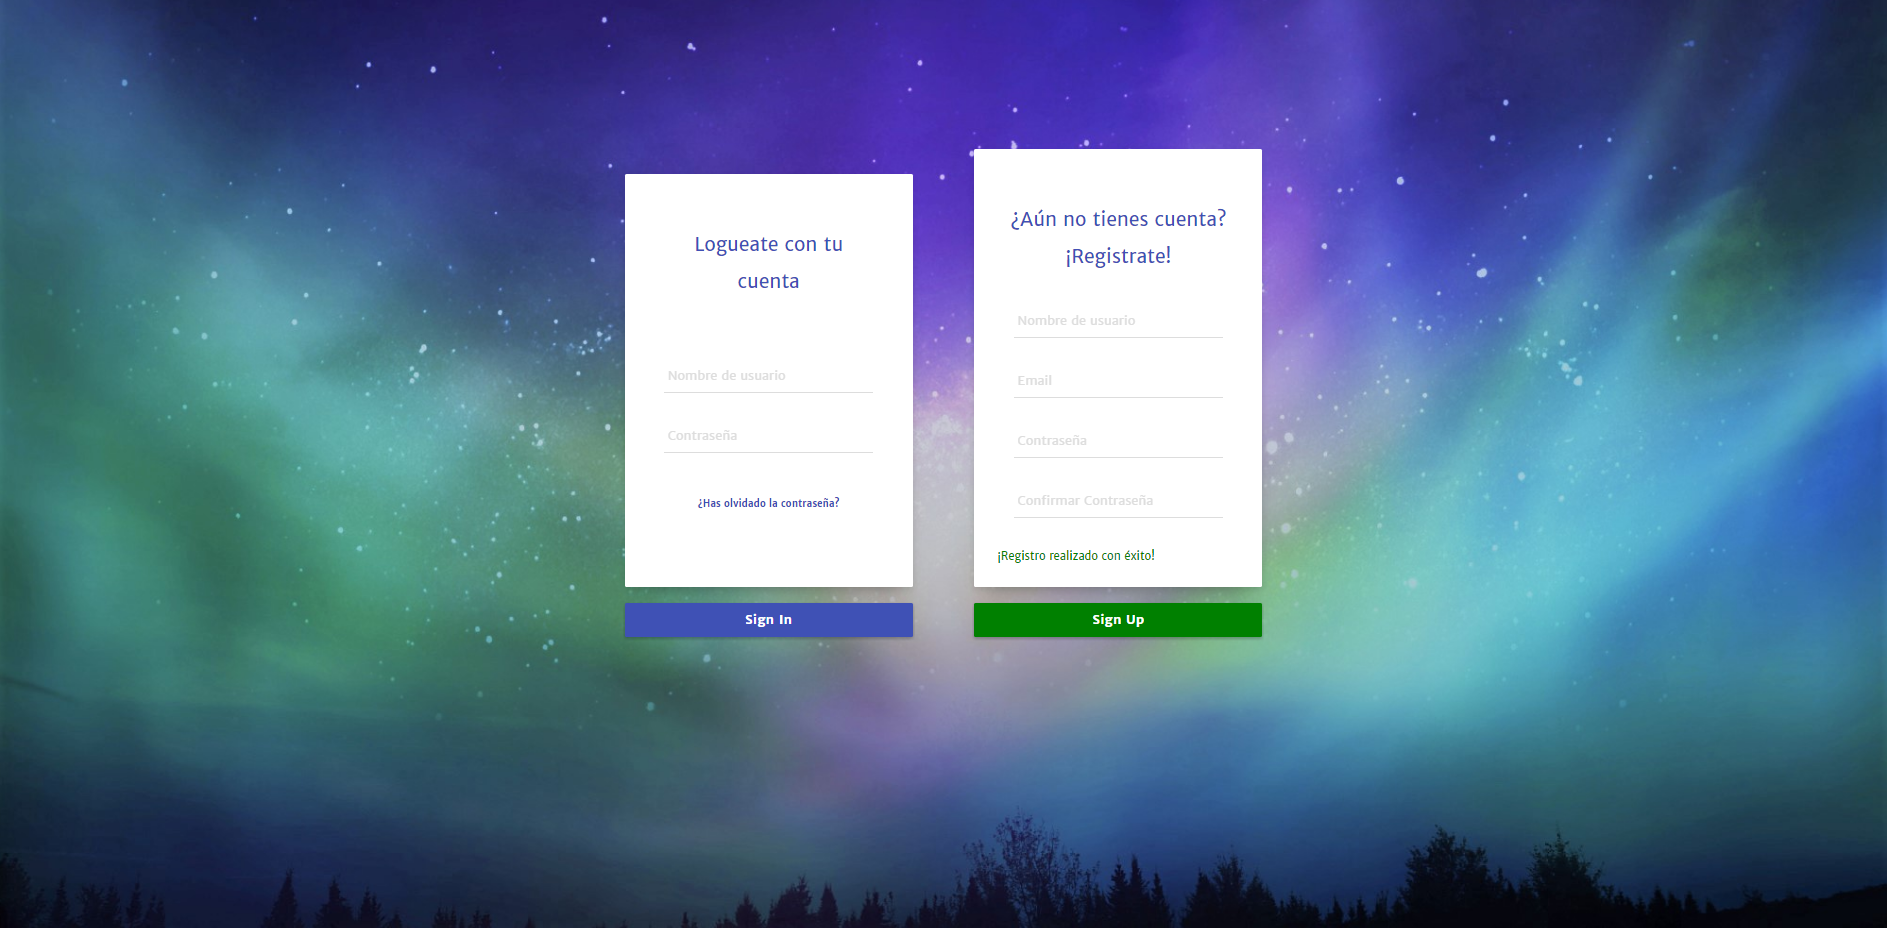
\includegraphics[totalheight=6cm]{manualUsuario/registroConExito.png}
\caption{Página de Inicio - Registro con éxito}
\end{figure}

\section{Login en la aplicación}

Para proceder al Login en la aplicación, accederemos a la Página de Inicio de ésta.

Una vez nos encontremos en la Página de Inicio, nos encontraremos con dos formularios. Para proceder al login deberemos de rellenar con datos correctos los datos del formulario de la izquierda y pulsar sobre el botón de ``Sign In''.

\begin{figure}[H]
\centering
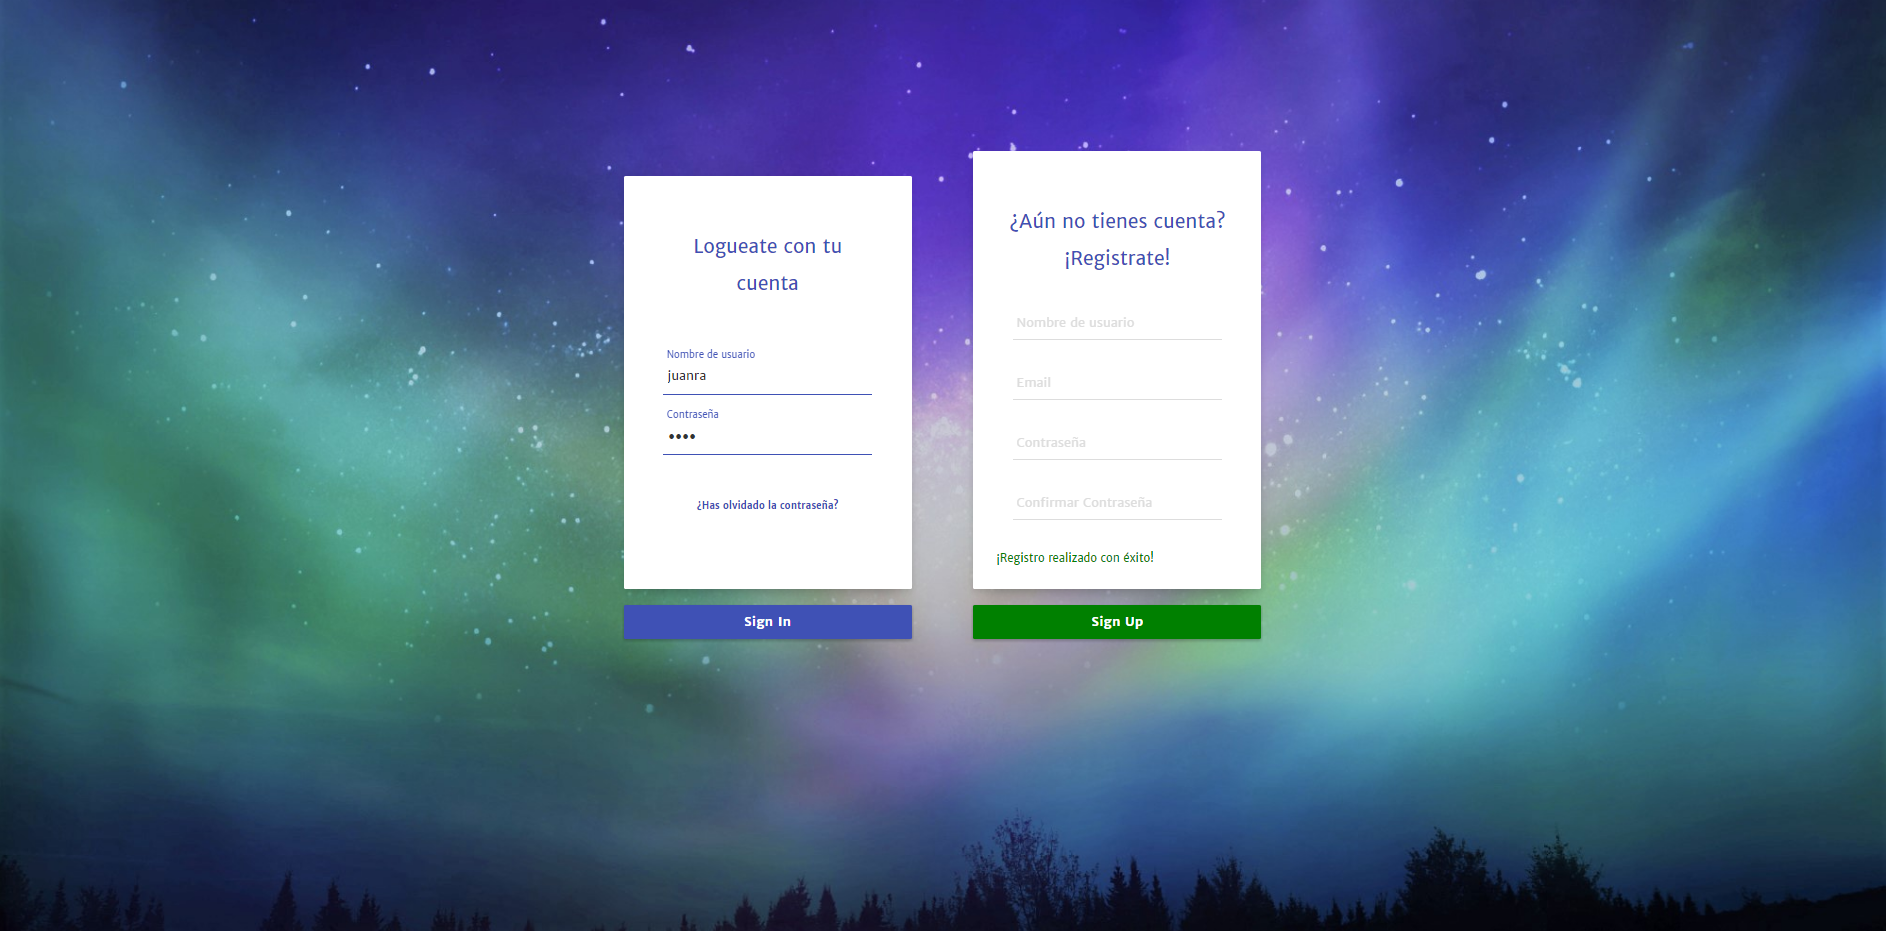
\includegraphics[totalheight=6cm]{manualUsuario/login.png}
\caption{Página de Inicio - Login}
\end{figure}

\pagebreak
Si se han seguido éstos pasos, la página redirigirá a la Página Principal. Una vez en ésta, nos encontraremos con un menú de usuario en la parte superior derecha, si hacemos ``click'' en dicho menú, tendremos la opción de ``LogOut'' la cual nos permitirá desloguearnos del sistema.

\begin{figure}[H]
\centering
\includegraphics[totalheight=6cm]{manualUsuario/logout.png}
\caption{Página de Inicio - Logout}
\end{figure}

\pagebreak
\section{Acceder a la Página Principal}

Para poder acceder a la Página Principal habrá que loguearse primero en la aplicación.

Una vez nos encontremos en la Página Principal, nos encontraremos con el logo de la aplicación, un menú de usuario en la parte superior derecha y un calendario que ocupará gran parte de la vista de la aplicación. En el menú podremos acceder a los distintos apartados que nos ofrece la aplicación. Respecto al calendario, podremos navegar entre los distintos meses o pulsar en el botón para volver al mes actual y en el interior del mismo podremos ver representados los eventos de sueño registrados en la aplicación. 

\begin{figure}[H]
\centering
\includegraphics[totalheight=6cm]{manualUsuario/paginaPrincipal.png}
\caption{Página Principal}
\end{figure}

\pagebreak
Haciendo ``click'' sobre cualquier día del calendario que contenga un evento, se nos desplegará un apartado con un enlace para acceder a la página ``Resumen de Sueño Diario'' con los detalles del mismo.

\begin{figure}[H]
\centering
\includegraphics[totalheight=6cm]{manualUsuario/eventos.png}
\caption{Página Principal - Eventos}
\end{figure}

\pagebreak
\section{Acceder a la página de ``Resumen de Sueño Diario''}

Para poder acceder a la página de ``Resumen de Sueño Diario'' habrá que encontrarse en la Página Principal con al menos un evento en el calendario.

\begin{figure}[H]
\centering
\includegraphics[totalheight=6cm]{manualUsuario/paginaPrincipal.png}
\caption{Página Principal}
\end{figure}

Una vez nos encontremos en la Página Principal con al menos un evento, haremos ``click'' sobre uno de los días que tengan un evento, desplegándose un menú bajo éste día. En el menú seleccionaremos el enlace que deseemos visitar y accederemos a la página de ``Resumen de Sueño Diario''.

\begin{figure}[H]
\centering
\includegraphics[totalheight=6cm]{manualUsuario/eventos.png}
\caption{Página Principal - Eventos}
\end{figure}

En ésta página, se nos mostrarán dos gráficas. La primera de ellas, nos mostrará los movimientos que han ocurrido durante la noche en un instante determinado. La segunda, nos mostrará que porcentaje hemos dormido en cada uno de los estados de sueño.

\begin{figure}[H]
\centering
\includegraphics[totalheight=6cm]{manualUsuario/resumenSue_oDiario.png}
\caption{Página de Resumen de Sueño Diario}
\end{figure}

\section{Manejar integraciones con las APIs de registro de sueño}

Para poder acceder a la página de APIs y manejar nuestras integraciones, habrá que encontrarse en la Página Principal.

\begin{figure}[H]
\centering
\includegraphics[totalheight=6cm]{manualUsuario/paginaPrincipal.png}
\caption{Página Principal}
\end{figure}

Una vez nos encontremos en la Página Principal, haremos ``click'' sobre el menú de Usuario situado en la parte superior derecha. De dicho menú se nos desplegaran una serie de opciones, de la que seleccionaremos la opción ``APIs''.

\begin{figure}[H]
\centering
\includegraphics[totalheight=6cm]{manualUsuario/apis.png}
\caption{Página Principal - APIs}
\end{figure}

Una vez seleccionemos la opción de ``APIs'', nos encontraremos ante la página de Integraciones con las APIs, en la que podremos manejar nuestras integraciones. En dicha página veremos varias imágenes que nos conducirán a los pasos necesarios para activar la integración con dicha API.

\begin{figure}[H]
\centering
\includegraphics[totalheight=6cm]{manualUsuario/paginaApis.png}
\caption{Página de Integraciones con las APIs}
\end{figure}

\section{Manejar alertas}

Para poder acceder a la página de Alertas y manejarlas, habrá que encontrarse en la Página Principal.

\begin{figure}[H]
\centering
\includegraphics[totalheight=6cm]{manualUsuario/paginaPrincipal.png}
\caption{Página Principal}
\end{figure}

Una vez nos encontremos en la Página Principal, haremos ``click'' sobre el menú de Usuario situado en la parte superior derecha. De dicho menú se nos desplegaran una serie de opciones, de la que seleccionaremos la opción ``Alertas''.

\begin{figure}[H]
\centering
\includegraphics[totalheight=6cm]{manualUsuario/alertas.png}
\caption{Página Principal - Alertas}
\end{figure}

Una vez seleccionemos la opción de ``Alertas'', nos encontraremos ante la página de Alertas, en la que podremos manejarlas. En dicha página se mostrará un texto explicándonos la funcionalidad y un formulario para activar las notificaciones y definir la regla de intervalos y horas a incumplir para que se nos notifique.

\begin{figure}[H]
\centering
\includegraphics[totalheight=6cm]{manualUsuario/paginaAlertas.png}
\caption{Página de Alertas}
\end{figure}

\section{Recuperación de contraseña}

Para recuperar la contraseña, deberemos encontrarnos en la Página de Inicio de la aplicación.

\begin{figure}[H]
\centering
\includegraphics[totalheight=6cm]{manualUsuario/paginaInicio.png}
\caption{Página de Inicio}
\end{figure}

En ésta página se nos mostrarán dos formularios. En el formulario de la derecha, correspondiente al formulario de login, se nos mostrará un enlace de: ``¿Has olvidado la contraseña?''. Si hacemos ``click'' sobre éste enlace, se nos redireccionará a una página en la que nos pedirá nuestro nombre de usuario.

\begin{figure}[H]
\centering
\includegraphics[totalheight=6cm]{manualUsuario/contrase_aOlvidada.png}
\caption{Página de Contraseña Olvidada}
\end{figure}

Deberemos de introducirlo y pulsar el botón ``Submit''. Una vez pulsado éste botón se nos redireccionará a una página indicándonos que se nos ha enviado un enlace de recuperación de contraseña al email asignado a nuestra cuenta (ésta dirección de email ira oculto en gran parte con la finalidad de que sólo el verdadero usuario sea capaz de reconocer cuál es).

\begin{figure}[H]
\centering
\includegraphics[totalheight=6cm]{manualUsuario/correoEnviado.png}
\caption{Página de Correo Enviado}
\end{figure}

\pagebreak
Al hacer ``click'' sobre el enlace que tendremos en nuestro correo, se nos redirigirá a una página de la aplicación en la que se nos pedirá que introduzcamos la nueva contraseña. La introduciremos y pulsaremos el botón ``Submit''. 

\begin{figure}[H]
\centering
\includegraphics[totalheight=6cm]{manualUsuario/correoRecibido.png}
\caption{Correo Recibido}
\end{figure}

\begin{figure}[H]
\centering
\includegraphics[totalheight=6cm]{manualUsuario/contrase_aRecuperacion.png}
\caption{Página de Recuperación de Contraseña}
\end{figure}

\pagebreak
Una vez realizados éstos pasos con éxito, se nos informará que nuestra contraseña ha sido restablecida con éxito y se nos invitará a loguearnos con la nueva contraseña en la aplicación.

\begin{figure}[H]
\centering
\includegraphics[totalheight=6cm]{manualUsuario/contrase_aRestablecida.png}
\caption{Página de Contraseña Restablecida}
\end{figure}

\pagebreak
\section{Navegabilidad}

A continuación se expone a modo resumen un diagrama con el flujo que se puede seguir para navegar entre las distintas páginas de la aplicación. Con dicho diagrama se pretende que el lector comprenda de un vistazo cuál es la estructura que puede visitar y cual es el flujo para navegar en dicha estructura.

\begin{figure}[H]
\centering
\includegraphics[totalheight=8cm]{manualUsuario/Navegabilidad.png}
\caption{Navegabilidad}
\end{figure}


% 8. Conclusiones
\chapter{Conclusiones}

Es el momento de abordar las conclusiones obtenidas tras la realización del Trabajo de Fin de Grado. Llegado a éste punto, si el lector ha seguido ordenadamente los distintos capítulos que se abordan en la memoria debería de tener una idea clara de cual ha sido la motivación, el desarrollo y la ejececución del TFG. Sin embargo, en éste apartado abordaremos algunos de ésos detalles con mayor precisión y se realizará una reflexión final.

Me gustaría comenzar destacando el hecho de que hemos completado con éxito los objetivos que nos propusimos al inicio del TFG, superando incluso las espectativas iniciales. Nuestros objetivos eran el de crear una aplicación para mostrar los datos de sueño de los usuarios empleando tecnologías innovadoras y con un mínimo de calidad a la altura de un Trabajo de Fin de Grado. Pues bien, hemos suplido con éxito estos requisitos, ya que la aplicación ha sido desarrollada siguiendo las tecnologías propuestas y es completamente funcional. Además, para asegurar algunos aspectos de la calidad del proyecto se han llevado a cabo las pruebas que se han visto en el Capítulo 6, con el objetivo de comprobar el funcionamiento de la aplicación.

Tras la ejecución del TFG he sacado la conclusión de que tomé la decisión correcta al elegir las tecnologías que he usado durante su desarrollo. El motivo de ésta conclusión es que he aprendido que tengo autonomía a la hora de conocer lenguajes completamente nuevos y que me desenvuelvo con ellos con algo de soltura. Además, éstos lenguajes me han hecho crecer como programador, ya que me han enseñado nuevos conceptos o me han hecho profundizar en algunos, como es el caso de la programación asincrona, la espera de eventos para realizar una acción o la utilización de ficheros tan simples como JSON para tareas no tan simples como el almacenamiento de datos en una Base de Datos.

Éstas tecnologías no sólo me han ayudado a adquirir conocimientos, si no que también me han ayudado a tener mayores expectativas sobre mi futuro, ya que gracias a su conocimiento se me abren ofertas que en otro caso hubiesen llevado un aprendizaje al que no todas las empresas están dispuestas. Son tecnologías en auge actualmente para el ámbito de desarrollo web, y ésto es de destacar, ya que es el ámbito al que me gustaría enfocar mi carrera profesional, otra de las motivaciones por la cual me decanté en la elección de éste TFG.

Respecto a la motivación con la idea principal, fue un problema personal que me surgió y en momentos no excesivamente amenos del transcurso del TFG, ya fuera por falta de tiempo o por que ésa parte del proyecto no me motivara especialmente, me ha ayudado a continuar con el mismo ímpetu como en otros momentos. La idea inicial era la de conseguir que una aplicación almacenar los datos no sólo del día anterior, si no un histórico de todos los días que se quisiera. He de reconocer que mi idea principal era mucho más sencilla que la que finalmente he desarrollado y no contemplaba la inclusión de otras tecnologías. Sin embargo, a pesar de requerir mayor esfuerzo, ha sido una motivación para mi, ya que veía como mi idea evolucionaba y se convertía una una mejor solución y más genérica, por lo que más personas con problemas similares al mío podrian verse beneficiadas de ella.

Tras probar distintas tecnologías para el desarrollo de aplicaciones web, he llegado a la conclusión que cada una están diseñadas con un enfoque más concreto a ciertos aspectos a pesar de que el ámbito sea el mismo. Tenía experiencia desarollando éste tipo de aplicaciones en Java, y tras probar Node.JS en lugar de Java para Backend, he llegado a la conclusión De que ambas tienen sus pros y sus contras. La elección de una u otra dependerá del tipo de proyecto, de la embergadura de éste y del alcance que se le quiera dar, mi conclusión es que ambas tecnologías son muy potentes para desarrollar aplicaciones web, decantándome más por Node.JS en la realización debido a mi curiosidad por conocer ésta tecnología y aprender más acerca de ella.

Acostumbrado a desarrollar sólo el BackEnd de las aplicaciones, el presente TFG me ha llevado a desarrollar ambas partes y vivir la experiencia de ser desarrollador tanto en BackEnd como en FrontEnd. La conclusión que he sacado al respecto es que ambas tareas son importantes y conllevan un esfuerzo considerable. Personalmente, sigo decantándome por el desarrollo en BackEnd. Sin embargo, la experiencia que he adquirido me ayudará en futuros proyectos en los que tenga que desarrollar en FrontEnd y me ayudará a desarrollarlos con mayor agilidad. Respecto al FrontEnd, gracias a teconologías como ``Angular Material'' he aprendido que actualmente se pueden desarrollar aplicaciones con un buen acabado sin necesidad de tener unos conocimientos muy avanzados. Librerías como éstas, agilizan mucho el proceso al contener componentes ya diseñados y modificables por el desarrollador y al suavizar en gran medida la curva de aprendizaje con lenguajes como CSS y JavaScript en el lado del cliente.

El presente Trabajo de Fin de Grado ha resultado para mi un reto. La necesidad de aprender nuevas tecnologías, el no tener un alcance del todo claro al inicio del mismo y la presión de tener que ejecutar su desarrollo con una planificación muy cuadrada para no cometer errores de planificación al final, ha supuesto un esfuerzo y un reto por mi parte que he asumido en la ejecución del mismo. Sin embargo, he sacado como conclusión que como todo esfuerzo o reto si se ejecuta como es debido se obtiene una recompensa, en mi caso la culminación de la ejecución del TFG y el poder tener una aplicación funcional y real, con la que además he aprendido y conocido nuevas tecnologías y estilos de programación que me pueden servir en un futuro. 

Respecto a la Base de Datos elegida, Firebase, creo que fue una decisión acertada. Firebase ha tenido un comportamiento estable y me ha permitido conocer el ámbito NOSQL. Éste ámbito es bastante popular actualmente gracias a algunas de las ventajas que tiene respecto a otros tipos de Bases de Datos. El contar con una empresa como Google respaldando su estabilidad me ha servido de apoyo, ya que no tenía que preocuparme del mantenimiento de la misma y podía despreocuparme de problemas como la caida de la Base de Datos durante el tiempo del desarrollo o que se corrompieran algunos de sus datos. Además considero que es una Base de Datos móvil con un gran potencial y que tiene una curva de aprendizaje muy suavizada, por lo que pienso que es recomendable para que cualquier desarrollador se inicie en este tipo de Bases de Datos y desarrolle aplicaciones gracias a ellas.

En las herramientas utilizadas para llevar a cabo el desarrollo, pienso que he elegido correctamente. Con Google Drive tenía experiencia anteriormente y sabía que podría suplir mis necesidades a la hora de documentar. Toggl la descrubrí gracias a la proposición de usar ésta tecnología que me hizo mi tutor, aunque tenía experiencia con herramientas similares. A pesar de ello, reconozco que es una herramienta que me cautivó y que intento utilizarla en todos los proyectos tanto personales, como educativos en los que me es posible, ya que me ha ayudado a llevar un control muy exacto y claro de en qué invertía mi tiempo, además de mostrar facilmente los resultados como vimos en el Cápitulo 4.

Pero sin duda, me he dejado el mayor descubrimiento para el final, hablo de Visual Studio Code. He de reconocer que tenía en mente utilizar otra herramienta de una empresa con la que tenía experiencias positivas en el Software que ofrecen. Visual Studio Code fue al igual que Toggl una recomendación de mi tutor, ya que es cada vez más usadas por los desarrolladores de Angular, y ése motivo y mi curiosidad por probar nuevas herramientas en mi desarrollo fue lo que me convenció. He llegado a la conclusión tras su uso durante la ejecución del TFG de que es una herramienta muy potente y versátil. Potente ya que suple muchas de las necesidades de los desarrolladores con funcionalidades de ``serie'', como la necesidad de una consola integrada, un cliente de gestor de versiones (principalmente ``git''), un apartado para el debug, un buscador de funcionalidades, y un largo etcétera. Versátil ya que gracias a sus extensiones se le pueden agregar muchas funcionalidades y sobre todo compatibilidad con un gran número de lenguajes, lo que me ha permitido desarrollar desde en Node.JS, hasta en CSS, como incluso en el lenguaje de la presente memoria, LaTeX. Tódos estos lenguajes soportados gracias al propio Code o a extensiones del mismo y no sólo dando las funcionalidades que podrían darnos un editor de texto plano.

En resumen, a lo largo del TFG he llegado a la conclusión de que todo el esfuerzo realizado ha merecido la pena, que los resultados obtenidos son mayores a los que deseaba en un principio y que mi curiosidad por aprender nuevas tecnologías se ha suplido con éxito. El camino que he recorrido me ha llevado a llegar a éstas conclusiones y al visualizar los resultados éstas se consolidan. Considero que he cumplido con mis propósitos respecto a lo que me ofrece la aplicación que he desarrollado y además, he conseguido superar las curvas de aprendizaje con éxito y solventar los problemas con los lenguajes y tecnologías que he ido encontrando por el camino. Por ello, me considero orgulloso del trabajo que he realizado y considero que incluso puede tener un ámbito más allá de su propia realización, pudiendo implantarse como una aplicación real que sea utilizada por las personas que lo necesiten.

No me gustaría terminar la presente memoria sin abordar los distintos agradecimientos a las personas que me han apoyado en el transcurso del Trabajo de Fin de Grado. Le doy las gracias a mi familia, la cual ha sabido apoyarme en todo momento y valorar el trabajo que estaba realizando, interesándose por el mismo y reconociendolo a nivel público. A mi madre que ha sabido recordarme a diario la necesidad de ejecutar el trabajo con éxito y produciendo buenos resultados, apoyándome en los momentos que lo he necesitado. A mi padre, el cual me enseyó a terminar las cosas que empiezo y que siempre hay un momento para hacer las cosas y no es coveniente que ése momento pase. A mi pareja, ya que me ha apoyado incondicionalmente y ha sabido ayudarme en los momentos en los que la he necesitado a mi lado, aguantándome en los momentos más duros del desarrollo y valorando mi trabajo desde el principio hasta el final del mismo. 

Pero por supuesto he de agradecerle el trabajo que ha ejercido sobre éste TFG mi tutor, ya que sin su motivación, sus ganas y sus ánimos el presente trabajo no hubiese sido posible. Él ha conseguido que consiguiera mis metas, no sólo ha ejercido como tutor, si no como asesor, como analista e incluso en algunas ocasiones como consejero, brindándome importantes ideas y mostrándome puntos de vista que no había considerado y que ampliaban el enfoque y el alcance de la aplicación. Parte de éste TFG es suyo ya que considero que las ideas son tanto o más importantes como la ejecución de las mismas. De nuevo agradezco a todas éstas personas su apoyo incondicional y espero haber podido compensar su apoyo con los resultados obtenidos. 


% 9. Referencias
\addcontentsline{toc}{chapter}{9. Referencias}
\begin{thebibliography}{References}
\bibitem{1} \textsc{¿Cuántas horas es aconsejable dormir según nuestra edad?} [\url{http://www.abc.es/familia-vida-sana/20150212/abci-dormir-horas-201502121131.html}]
\bibitem{2} \textsc{JavaScript} [\url{https://es.wikipedia.org/wiki/JavaScript}]
\bibitem{3} \textsc{TypeScript} [\url{https://es.wikipedia.org/wiki/TypeScript}]
\bibitem{4} \textsc{Node.js} [\url{https://es.wikipedia.org/wiki/Node.js}]
\bibitem{5} \textsc{Express.js} [\url{https://en.wikipedia.org/wiki/Express.js}]
\bibitem{6} \textsc{Angular2} [\url{https://www.tutorialspoint.com/angular2/}]
\bibitem{7} \textsc{Firebase} [\url{https://en.wikipedia.org/wiki/Firebase}]
\bibitem{8} \textsc{Firebase (Github)} [\url{https://github.com/firebase/}]
\bibitem{9} \textsc{Selenium} [\url{ttps://es.wikipedia.org/wiki/Selenium}]
\bibitem{10} \textsc{Jasmine} [\url{ttps://en.wikipedia.org/wiki/Jasmine_(JavaScript_testing_framework)}]
\bibitem{11} \textsc{Protractor} [\url{https://www.adictosaltrabajo.com/tutoriales/introduccion-a-protractor/}]
\bibitem{12} \textsc{Visual Studio Code} [\url{ttps://en.wikipedia.org/wiki/Visual_Studio_Code}]
\bibitem{13} \textsc{Scrum: The Art of Doing Twice the Work in Half the Time} [Autor: Jeff Sutherland]
\bibitem{14} \textsc{UML Distilled} [Autor: Martin Fowler]
\bibitem{15} \textsc{Travis} [\url{https://en.wikipedia.org/wiki/Travis_CI}]
\bibitem{16} \textsc{Sprint} [\url{https://proyectosagiles.org/ejecucion-iteracion-sprint/}]
\bibitem{17} \textsc{¿Cada cuánto solemos renovar el móvil en España?} [\url{http://byemovil.com/renovar-el-movil}]
\bibitem{18} \textsc{Understanding Model-View-Controller} [Autor: Stefano Borini \url{https://www.gitbook.com/book/stefanoborini/modelviewcontroller/details}]

\end{thebibliography}

\appendix %% Up to you -- I just like to have the end notes as an appendix :-)
\printnotes*

\end{document}